% Options for packages loaded elsewhere
\PassOptionsToPackage{unicode}{hyperref}
\PassOptionsToPackage{hyphens}{url}
%
\documentclass[
]{book}
\usepackage{amsmath,amssymb}
\usepackage{lmodern}
\usepackage{iftex}
\ifPDFTeX
  \usepackage[T1]{fontenc}
  \usepackage[utf8]{inputenc}
  \usepackage{textcomp} % provide euro and other symbols
\else % if luatex or xetex
  \usepackage{unicode-math}
  \defaultfontfeatures{Scale=MatchLowercase}
  \defaultfontfeatures[\rmfamily]{Ligatures=TeX,Scale=1}
\fi
% Use upquote if available, for straight quotes in verbatim environments
\IfFileExists{upquote.sty}{\usepackage{upquote}}{}
\IfFileExists{microtype.sty}{% use microtype if available
  \usepackage[]{microtype}
  \UseMicrotypeSet[protrusion]{basicmath} % disable protrusion for tt fonts
}{}
\makeatletter
\@ifundefined{KOMAClassName}{% if non-KOMA class
  \IfFileExists{parskip.sty}{%
    \usepackage{parskip}
  }{% else
    \setlength{\parindent}{0pt}
    \setlength{\parskip}{6pt plus 2pt minus 1pt}}
}{% if KOMA class
  \KOMAoptions{parskip=half}}
\makeatother
\usepackage{xcolor}
\usepackage{color}
\usepackage{fancyvrb}
\newcommand{\VerbBar}{|}
\newcommand{\VERB}{\Verb[commandchars=\\\{\}]}
\DefineVerbatimEnvironment{Highlighting}{Verbatim}{commandchars=\\\{\}}
% Add ',fontsize=\small' for more characters per line
\usepackage{framed}
\definecolor{shadecolor}{RGB}{248,248,248}
\newenvironment{Shaded}{\begin{snugshade}}{\end{snugshade}}
\newcommand{\AlertTok}[1]{\textcolor[rgb]{0.94,0.16,0.16}{#1}}
\newcommand{\AnnotationTok}[1]{\textcolor[rgb]{0.56,0.35,0.01}{\textbf{\textit{#1}}}}
\newcommand{\AttributeTok}[1]{\textcolor[rgb]{0.77,0.63,0.00}{#1}}
\newcommand{\BaseNTok}[1]{\textcolor[rgb]{0.00,0.00,0.81}{#1}}
\newcommand{\BuiltInTok}[1]{#1}
\newcommand{\CharTok}[1]{\textcolor[rgb]{0.31,0.60,0.02}{#1}}
\newcommand{\CommentTok}[1]{\textcolor[rgb]{0.56,0.35,0.01}{\textit{#1}}}
\newcommand{\CommentVarTok}[1]{\textcolor[rgb]{0.56,0.35,0.01}{\textbf{\textit{#1}}}}
\newcommand{\ConstantTok}[1]{\textcolor[rgb]{0.00,0.00,0.00}{#1}}
\newcommand{\ControlFlowTok}[1]{\textcolor[rgb]{0.13,0.29,0.53}{\textbf{#1}}}
\newcommand{\DataTypeTok}[1]{\textcolor[rgb]{0.13,0.29,0.53}{#1}}
\newcommand{\DecValTok}[1]{\textcolor[rgb]{0.00,0.00,0.81}{#1}}
\newcommand{\DocumentationTok}[1]{\textcolor[rgb]{0.56,0.35,0.01}{\textbf{\textit{#1}}}}
\newcommand{\ErrorTok}[1]{\textcolor[rgb]{0.64,0.00,0.00}{\textbf{#1}}}
\newcommand{\ExtensionTok}[1]{#1}
\newcommand{\FloatTok}[1]{\textcolor[rgb]{0.00,0.00,0.81}{#1}}
\newcommand{\FunctionTok}[1]{\textcolor[rgb]{0.00,0.00,0.00}{#1}}
\newcommand{\ImportTok}[1]{#1}
\newcommand{\InformationTok}[1]{\textcolor[rgb]{0.56,0.35,0.01}{\textbf{\textit{#1}}}}
\newcommand{\KeywordTok}[1]{\textcolor[rgb]{0.13,0.29,0.53}{\textbf{#1}}}
\newcommand{\NormalTok}[1]{#1}
\newcommand{\OperatorTok}[1]{\textcolor[rgb]{0.81,0.36,0.00}{\textbf{#1}}}
\newcommand{\OtherTok}[1]{\textcolor[rgb]{0.56,0.35,0.01}{#1}}
\newcommand{\PreprocessorTok}[1]{\textcolor[rgb]{0.56,0.35,0.01}{\textit{#1}}}
\newcommand{\RegionMarkerTok}[1]{#1}
\newcommand{\SpecialCharTok}[1]{\textcolor[rgb]{0.00,0.00,0.00}{#1}}
\newcommand{\SpecialStringTok}[1]{\textcolor[rgb]{0.31,0.60,0.02}{#1}}
\newcommand{\StringTok}[1]{\textcolor[rgb]{0.31,0.60,0.02}{#1}}
\newcommand{\VariableTok}[1]{\textcolor[rgb]{0.00,0.00,0.00}{#1}}
\newcommand{\VerbatimStringTok}[1]{\textcolor[rgb]{0.31,0.60,0.02}{#1}}
\newcommand{\WarningTok}[1]{\textcolor[rgb]{0.56,0.35,0.01}{\textbf{\textit{#1}}}}
\usepackage{longtable,booktabs,array}
\usepackage{calc} % for calculating minipage widths
% Correct order of tables after \paragraph or \subparagraph
\usepackage{etoolbox}
\makeatletter
\patchcmd\longtable{\par}{\if@noskipsec\mbox{}\fi\par}{}{}
\makeatother
% Allow footnotes in longtable head/foot
\IfFileExists{footnotehyper.sty}{\usepackage{footnotehyper}}{\usepackage{footnote}}
\makesavenoteenv{longtable}
\usepackage{graphicx}
\makeatletter
\def\maxwidth{\ifdim\Gin@nat@width>\linewidth\linewidth\else\Gin@nat@width\fi}
\def\maxheight{\ifdim\Gin@nat@height>\textheight\textheight\else\Gin@nat@height\fi}
\makeatother
% Scale images if necessary, so that they will not overflow the page
% margins by default, and it is still possible to overwrite the defaults
% using explicit options in \includegraphics[width, height, ...]{}
\setkeys{Gin}{width=\maxwidth,height=\maxheight,keepaspectratio}
% Set default figure placement to htbp
\makeatletter
\def\fps@figure{htbp}
\makeatother
\setlength{\emergencystretch}{3em} % prevent overfull lines
\providecommand{\tightlist}{%
  \setlength{\itemsep}{0pt}\setlength{\parskip}{0pt}}
\setcounter{secnumdepth}{5}
\usepackage{booktabs}
\ifLuaTeX
  \usepackage{selnolig}  % disable illegal ligatures
\fi
\usepackage[]{natbib}
\bibliographystyle{plainnat}
\IfFileExists{bookmark.sty}{\usepackage{bookmark}}{\usepackage{hyperref}}
\IfFileExists{xurl.sty}{\usepackage{xurl}}{} % add URL line breaks if available
\urlstyle{same} % disable monospaced font for URLs
\hypersetup{
  pdftitle={Microbial Bile Acid Metabolism Shapes T Cell Responses During Inflammation},
  pdfauthor={Oriana Miltiadous},
  hidelinks,
  pdfcreator={LaTeX via pandoc}}

\title{Microbial Bile Acid Metabolism Shapes T Cell Responses During Inflammation}
\author{Oriana Miltiadous}
\date{2023-08-07}

\begin{document}
\maketitle

{
\setcounter{tocdepth}{1}
\tableofcontents
}
\hypertarget{introduction-load-the-datasets}{%
\chapter{Introduction: load the datasets}\label{introduction-load-the-datasets}}

\hypertarget{load-packages}{%
\section{Load packages}\label{load-packages}}

\begin{Shaded}
\begin{Highlighting}[]
\FunctionTok{library}\NormalTok{(janitor)}
\FunctionTok{library}\NormalTok{(readxl)}
\FunctionTok{library}\NormalTok{(tidyverse)}
\FunctionTok{library}\NormalTok{(ggpubr)}
\FunctionTok{library}\NormalTok{(data.table)}
\end{Highlighting}
\end{Shaded}

\hypertarget{load-datasets}{%
\section{Load datasets}\label{load-datasets}}

\begin{Shaded}
\begin{Highlighting}[]
\CommentTok{\#patient cohort}
\NormalTok{cohort\_BAS}\OtherTok{\textless{}{-}}\FunctionTok{read\_csv}\NormalTok{(}\StringTok{"/Volumes/vandenbrinklab/Oriana/BAs\_published\_datasets/cohort\_BAS.csv"}\NormalTok{)}
\NormalTok{ursodiol}\OtherTok{\textless{}{-}}\FunctionTok{read\_csv}\NormalTok{(}\StringTok{"/Volumes/vandenbrinklab/Oriana/BAs\_published\_datasets/ursodiol.csv"}\NormalTok{)}

\CommentTok{\#metabolomics data}
\CommentTok{\#concentrations}
\NormalTok{conc\_all\_filtered}\OtherTok{\textless{}{-}}\FunctionTok{read\_csv}\NormalTok{(}\StringTok{"/Volumes/vandenbrinklab/Oriana/BAs\_published\_datasets/conc\_all\_filtered.csv"}\NormalTok{)}
\NormalTok{filtered\_combined\_table}\OtherTok{\textless{}{-}}\FunctionTok{read\_csv}\NormalTok{(}\StringTok{"/Volumes/vandenbrinklab/Oriana/BAs\_published\_datasets/filtered\_combined\_table.csv"}\NormalTok{)}
\CommentTok{\#annotations}
\NormalTok{ba\_families}\OtherTok{\textless{}{-}}\FunctionTok{read\_csv}\NormalTok{(}\StringTok{"/Volumes/vandenbrinklab/Oriana/BAs\_published\_datasets/ba\_families.csv"}\NormalTok{)}

\CommentTok{\#16s data}
\NormalTok{counts\_samples }\OtherTok{\textless{}{-}}\FunctionTok{read\_csv}\NormalTok{(}\StringTok{"/Volumes/vandenbrinklab/Oriana/BAs\_published\_datasets/counts\_samples.csv"}\NormalTok{)}
\NormalTok{asv\_annotation\_blast\_ag}\OtherTok{\textless{}{-}}\FunctionTok{read\_csv}\NormalTok{(}\StringTok{"/Volumes/vandenbrinklab/Oriana/BAs\_published\_datasets/asv\_annotation\_blast\_ag.csv"}\NormalTok{)}
\NormalTok{asv\_alpha\_all}\OtherTok{\textless{}{-}}\FunctionTok{read\_csv}\NormalTok{(}\StringTok{"/Volumes/vandenbrinklab/Oriana/BAs\_published\_datasets/asv\_alpha\_all.csv"}\NormalTok{)}
\NormalTok{asv\_annotation\_blast\_color\_ag}\OtherTok{\textless{}{-}}\FunctionTok{read\_csv}\NormalTok{(}\StringTok{"/Volumes/vandenbrinklab/Oriana/BAs\_published\_datasets/asv\_annotation\_blast\_color\_ag.csv"}\NormalTok{)}

\CommentTok{\#shotgun data}
\NormalTok{BSH\_metalphlan }\OtherTok{\textless{}{-}}\FunctionTok{read\_csv}\NormalTok{(}\StringTok{"/Volumes/vandenbrinklab/Oriana/BAs\_published\_datasets/BSH\_metalphlan.csv"}\NormalTok{)}
\NormalTok{bai\_genes\_clean}\OtherTok{\textless{}{-}}\FunctionTok{read\_csv}\NormalTok{(}\StringTok{"/Volumes/vandenbrinklab/Oriana/BAs\_published\_datasets/bai\_genes\_clean.csv"}\NormalTok{)}
\NormalTok{taxa\_bas\_later}\OtherTok{\textless{}{-}}\FunctionTok{read\_csv}\NormalTok{(}\StringTok{"/Volumes/vandenbrinklab/Oriana/BAs\_published\_datasets/taxa\_bas\_later.csv"}\NormalTok{)}

\CommentTok{\#ursodiol cohort: double check that it\textquotesingle{}s ok to share}
\NormalTok{patients\_urso\_CIF}\OtherTok{\textless{}{-}} \FunctionTok{read\_csv}\NormalTok{( }\StringTok{"/Volumes/vandenbrinklab/Oriana/BAs\_published\_datasets/patients\_urso\_CIF.csv"}\NormalTok{)}
\end{Highlighting}
\end{Shaded}

\hypertarget{analyze-the-effect-of-udca-administration-on-the-bile-acid-pool-supplementary-figure-5}{%
\chapter{Analyze the effect of UDCA administration on the bile acid pool (supplementary figure 5)}\label{analyze-the-effect-of-udca-administration-on-the-bile-acid-pool-supplementary-figure-5}}

\begin{Shaded}
\begin{Highlighting}[]
\CommentTok{\#summarize bile acid pools}
\NormalTok{both\_conc}\OtherTok{\textless{}{-}}\NormalTok{ cohort\_BAS }\SpecialCharTok{\%\textgreater{}\%} \FunctionTok{select}\NormalTok{(}\SpecialCharTok{{-}}\NormalTok{ursodiol)}\SpecialCharTok{\%\textgreater{}\%}
  \FunctionTok{left\_join}\NormalTok{(conc\_all\_filtered) }\SpecialCharTok{\%\textgreater{}\%} \FunctionTok{clean\_names}\NormalTok{()}

\CommentTok{\#prep dataset prepping each BA depending on its classifications}
\NormalTok{both\_conc\_pools}\OtherTok{\textless{}{-}}\NormalTok{both\_conc }\SpecialCharTok{\%\textgreater{}\%} 
  \FunctionTok{gather}\NormalTok{(}\StringTok{"bile\_acid"}\NormalTok{, }\StringTok{"value"}\NormalTok{, }\FunctionTok{names}\NormalTok{(.)[}\DecValTok{8}\NormalTok{]}\SpecialCharTok{:}\FunctionTok{names}\NormalTok{(.)[}\FunctionTok{ncol}\NormalTok{(.)]) }\SpecialCharTok{\%\textgreater{}\%} 
  \FunctionTok{select}\NormalTok{(}\SpecialCharTok{{-}}\NormalTok{gi\_gvhd, }\SpecialCharTok{{-}}\NormalTok{later, }\SpecialCharTok{{-}}\NormalTok{periengr) }\SpecialCharTok{\%\textgreater{}\%} 
  \FunctionTok{left\_join}\NormalTok{(ba\_families) }\SpecialCharTok{\%\textgreater{}\%} 
  \FunctionTok{filter}\NormalTok{(bile\_acid}\SpecialCharTok{!=}\StringTok{"beta\_muricholic\_acid"}\NormalTok{) }\SpecialCharTok{\%\textgreater{}\%} \CommentTok{\#removing because it\textquotesingle{}s not measured in all samples}
  \FunctionTok{filter}\NormalTok{(bile\_acid}\SpecialCharTok{!=}\StringTok{"omega\_muricholic\_acid"}\NormalTok{) }\SpecialCharTok{\%\textgreater{}\%}  \CommentTok{\#removing because it\textquotesingle{}s not measured in all samples}
  \FunctionTok{mutate}\NormalTok{(}\AttributeTok{primary\_pool=}\FunctionTok{ifelse}\NormalTok{(prim\_vs\_sec}\SpecialCharTok{==}\StringTok{"Primary"}\NormalTok{, value, }\DecValTok{0}\NormalTok{)) }\SpecialCharTok{\%\textgreater{}\%} 
  \FunctionTok{mutate}\NormalTok{(}\AttributeTok{secondary\_pool=}\FunctionTok{ifelse}\NormalTok{(prim\_vs\_sec}\SpecialCharTok{==}\StringTok{"Secondary"}\NormalTok{, value, }\DecValTok{0}\NormalTok{)) }\SpecialCharTok{\%\textgreater{}\%} 
  \FunctionTok{mutate}\NormalTok{(}\AttributeTok{sulfated\_pool=}\FunctionTok{ifelse}\NormalTok{(sulfated}\SpecialCharTok{==}\StringTok{"Y"}\NormalTok{, value, }\DecValTok{0}\NormalTok{)) }\SpecialCharTok{\%\textgreater{}\%} 
  \FunctionTok{mutate}\NormalTok{(}\AttributeTok{conjugated\_pool=}\FunctionTok{ifelse}\NormalTok{(amidated}\SpecialCharTok{==}\StringTok{"Y"} \SpecialCharTok{\&}\NormalTok{ sulfated}\SpecialCharTok{==}\StringTok{"N"}\NormalTok{, value, }\DecValTok{0}\NormalTok{)) }\SpecialCharTok{\%\textgreater{}\%} 
  \FunctionTok{mutate}\NormalTok{(}\AttributeTok{unconjugated\_pool=}\FunctionTok{ifelse}\NormalTok{(amidated}\SpecialCharTok{==}\StringTok{"N"} \SpecialCharTok{\&}\NormalTok{ sulfated}\SpecialCharTok{==}\StringTok{"N"}\NormalTok{, value, }\DecValTok{0}\NormalTok{)) }\SpecialCharTok{\%\textgreater{}\%} 
  \FunctionTok{mutate}\NormalTok{(}\AttributeTok{secondary\_nonUDCA=}\FunctionTok{ifelse}\NormalTok{(prim\_vs\_sec}\SpecialCharTok{==}\StringTok{"Secondary"} \SpecialCharTok{\&}\NormalTok{ udca}\SpecialCharTok{==}\StringTok{"N"}\NormalTok{, value, }\DecValTok{0}\NormalTok{)) }\SpecialCharTok{\%\textgreater{}\%} 
  \FunctionTok{mutate}\NormalTok{(}\AttributeTok{total\_BAs=}\NormalTok{value) }\SpecialCharTok{\%\textgreater{}\%} 
  \FunctionTok{mutate}\NormalTok{(}\AttributeTok{total\_nonUDCA\_pool=}\FunctionTok{ifelse}\NormalTok{(udca}\SpecialCharTok{==}\StringTok{"N"}\NormalTok{, value, }\DecValTok{0}\NormalTok{)) }\SpecialCharTok{\%\textgreater{}\%} 
  \FunctionTok{mutate}\NormalTok{(}\AttributeTok{glycine\_pool=}\FunctionTok{ifelse}\NormalTok{(glycine}\SpecialCharTok{==}\StringTok{"Y"} \SpecialCharTok{\&}\NormalTok{ sulfated}\SpecialCharTok{==}\StringTok{"N"}\NormalTok{, value, }\DecValTok{0}\NormalTok{)) }\SpecialCharTok{\%\textgreater{}\%} 
  \FunctionTok{mutate}\NormalTok{(}\AttributeTok{taurine\_pool=}\FunctionTok{ifelse}\NormalTok{(taurine}\SpecialCharTok{==}\StringTok{"Y"} \SpecialCharTok{\&}\NormalTok{ sulfated}\SpecialCharTok{==}\StringTok{"N"}\NormalTok{, value, }\DecValTok{0}\NormalTok{)) }\SpecialCharTok{\%\textgreater{}\%} 
  \FunctionTok{mutate}\NormalTok{(}\AttributeTok{taurine\_SBA\_pool=}\FunctionTok{ifelse}\NormalTok{(taurine}\SpecialCharTok{==}\StringTok{"Y"} \SpecialCharTok{\&}\NormalTok{ prim\_vs\_sec}\SpecialCharTok{==}\StringTok{"Secondary"} \SpecialCharTok{\&}\NormalTok{ sulfated}\SpecialCharTok{==}\StringTok{"N"}\NormalTok{, value, }\DecValTok{0}\NormalTok{)) }\SpecialCharTok{\%\textgreater{}\%} 
  \FunctionTok{mutate}\NormalTok{(}\AttributeTok{taurine\_PBA\_pool=}\FunctionTok{ifelse}\NormalTok{(taurine}\SpecialCharTok{==}\StringTok{"Y"} \SpecialCharTok{\&}\NormalTok{ prim\_vs\_sec}\SpecialCharTok{==}\StringTok{"Primary"} \SpecialCharTok{\&}\NormalTok{ sulfated}\SpecialCharTok{==}\StringTok{"N"}\NormalTok{, value, }\DecValTok{0}\NormalTok{)) }\SpecialCharTok{\%\textgreater{}\%} 
  \FunctionTok{mutate}\NormalTok{(}\AttributeTok{glycine\_SBA\_pool=}\FunctionTok{ifelse}\NormalTok{(glycine}\SpecialCharTok{==}\StringTok{"Y"}\SpecialCharTok{\&}\NormalTok{ prim\_vs\_sec}\SpecialCharTok{==}\StringTok{"Secondary"} \SpecialCharTok{\&}\NormalTok{ sulfated}\SpecialCharTok{==}\StringTok{"N"}\NormalTok{, value, }\DecValTok{0}\NormalTok{)) }\SpecialCharTok{\%\textgreater{}\%} 
  \FunctionTok{mutate}\NormalTok{(}\AttributeTok{glycine\_PBA\_pool=}\FunctionTok{ifelse}\NormalTok{(glycine}\SpecialCharTok{==}\StringTok{"Y"} \SpecialCharTok{\&}\NormalTok{prim\_vs\_sec}\SpecialCharTok{==}\StringTok{"Primary"}\SpecialCharTok{\&}\NormalTok{ sulfated}\SpecialCharTok{==}\StringTok{"N"}\NormalTok{, value, }\DecValTok{0}\NormalTok{)) }\SpecialCharTok{\%\textgreater{}\%} 
  \FunctionTok{select}\NormalTok{(}\SpecialCharTok{{-}}\FunctionTok{colnames}\NormalTok{(ba\_families), }\SpecialCharTok{{-}}\NormalTok{value) }

\NormalTok{both\_conc\_pools\_final}\OtherTok{\textless{}{-}}\NormalTok{both\_conc\_pools }\SpecialCharTok{\%\textgreater{}\%} 
  \FunctionTok{group\_by}\NormalTok{(sampleid) }\SpecialCharTok{\%\textgreater{}\%} 
  \FunctionTok{summarise}\NormalTok{(}\FunctionTok{across}\NormalTok{(}\FunctionTok{where}\NormalTok{(is.numeric), sum)) }\SpecialCharTok{\%\textgreater{}\%} 
  \FunctionTok{left\_join}\NormalTok{(ursodiol)}

\CommentTok{\#rearrange ursodiol}
\NormalTok{both\_conc\_pools\_final}\SpecialCharTok{$}\NormalTok{ursodiol }\OtherTok{\textless{}{-}}\FunctionTok{factor}\NormalTok{(both\_conc\_pools\_final}\SpecialCharTok{$}\NormalTok{ursodiol, }
                           \AttributeTok{levels=}\FunctionTok{c}\NormalTok{(}\StringTok{"Y"}\NormalTok{,}\StringTok{"2{-}3w"}\NormalTok{,}\StringTok{"3{-}4w"}\NormalTok{,}\StringTok{"1{-}2m"}\NormalTok{, }\StringTok{"N"}\NormalTok{))}
\end{Highlighting}
\end{Shaded}

\#\#Evaluation of ursodiol exposure and UDCA concentration

\begin{Shaded}
\begin{Highlighting}[]
\NormalTok{ursodiol\_BAs}\OtherTok{\textless{}{-}}\NormalTok{both\_conc }\SpecialCharTok{\%\textgreater{}\%} 
  \FunctionTok{left\_join}\NormalTok{(ursodiol)}
  
\CommentTok{\#rearrange ursodiol}
\NormalTok{ursodiol\_BAs}\SpecialCharTok{$}\NormalTok{ursodiol }\OtherTok{\textless{}{-}}\FunctionTok{factor}\NormalTok{(ursodiol\_BAs}\SpecialCharTok{$}\NormalTok{ursodiol, }
                           \AttributeTok{levels=}\FunctionTok{c}\NormalTok{(}\StringTok{"Y"}\NormalTok{,}\StringTok{"2{-}3w"}\NormalTok{,}\StringTok{"3{-}4w"}\NormalTok{,}\StringTok{"1{-}2m"}\NormalTok{, }\StringTok{"N"}\NormalTok{))}

\NormalTok{ursodiol\_BAs }\SpecialCharTok{\%\textgreater{}\%} 
  \FunctionTok{ggplot}\NormalTok{(}\FunctionTok{aes}\NormalTok{(}\AttributeTok{x=}\NormalTok{ursodiol, }\AttributeTok{y=}\FunctionTok{log10}\NormalTok{(}\StringTok{\textasciigrave{}}\AttributeTok{ursodeoxycholic\_acid}\StringTok{\textasciigrave{}}\NormalTok{), }\AttributeTok{color=}\NormalTok{ursodiol)) }\SpecialCharTok{+}
  \FunctionTok{geom\_boxplot}\NormalTok{(}\AttributeTok{width=}\FloatTok{0.2}\NormalTok{, }\AttributeTok{outlier.shape =}\ConstantTok{NA}\NormalTok{, }\AttributeTok{lwd=}\NormalTok{.}\DecValTok{7}\NormalTok{)}\SpecialCharTok{+}
  \FunctionTok{geom\_jitter}\NormalTok{(}\AttributeTok{width=}\FloatTok{0.2}\NormalTok{, }\AttributeTok{alpha=}\FloatTok{0.2}\NormalTok{)}\SpecialCharTok{+}
  \FunctionTok{theme\_classic}\NormalTok{() }\SpecialCharTok{+}
  \FunctionTok{xlab}\NormalTok{(}\StringTok{"ursodiol exposure"}\NormalTok{)}\SpecialCharTok{+}
  \FunctionTok{stat\_compare\_means}\NormalTok{(}\AttributeTok{comparisons=}\FunctionTok{list}\NormalTok{( }\FunctionTok{c}\NormalTok{(}\StringTok{"Y"}\NormalTok{, }\StringTok{"2{-}3w"}\NormalTok{),}\FunctionTok{c}\NormalTok{(}\StringTok{"3{-}4w"}\NormalTok{, }\StringTok{"Y"}\NormalTok{), }\FunctionTok{c}\NormalTok{(}\StringTok{"Y"}\NormalTok{, }\StringTok{"1{-}2m"}\NormalTok{), }\FunctionTok{c}\NormalTok{(}\StringTok{"N"}\NormalTok{, }\StringTok{"Y"}\NormalTok{),}
                                       \FunctionTok{c}\NormalTok{(}\StringTok{"3{-}4w"}\NormalTok{, }\StringTok{"2{-}3w"}\NormalTok{),}\FunctionTok{c}\NormalTok{(}\StringTok{"1{-}2m"}\NormalTok{, }\StringTok{"2{-}3w"}\NormalTok{), }\FunctionTok{c}\NormalTok{(}\StringTok{"N"}\NormalTok{, }\StringTok{"2{-}3w"}\NormalTok{),}
                                       \FunctionTok{c}\NormalTok{(}\StringTok{"1{-}2m"}\NormalTok{, }\StringTok{"3{-}4w"}\NormalTok{),  }\FunctionTok{c}\NormalTok{(}\StringTok{"N"}\NormalTok{, }\StringTok{"3{-}4w"}\NormalTok{),}
                                       \FunctionTok{c}\NormalTok{(}\StringTok{"N"}\NormalTok{, }\StringTok{"1{-}2m"}\NormalTok{)}
\NormalTok{  ),}
  \CommentTok{\#label="p.signif",}
  \AttributeTok{method=}\StringTok{"wilcox.test"}\NormalTok{,}
  \AttributeTok{correct=}\ConstantTok{FALSE}\NormalTok{)}\SpecialCharTok{+}
  \FunctionTok{scale\_color\_manual}\NormalTok{(}\AttributeTok{values=}\FunctionTok{c}\NormalTok{(}\StringTok{"\#a6611a"}\NormalTok{, }\StringTok{"\#bf812d"}\NormalTok{,}\StringTok{"\#dfc27d"}\NormalTok{, }\StringTok{"\#80cdc1"}\NormalTok{, }\StringTok{"\#018571"}\NormalTok{))}\SpecialCharTok{+}
  \FunctionTok{theme}\NormalTok{(}\AttributeTok{legend.position=}\StringTok{"none"}\NormalTok{)}
\end{Highlighting}
\end{Shaded}

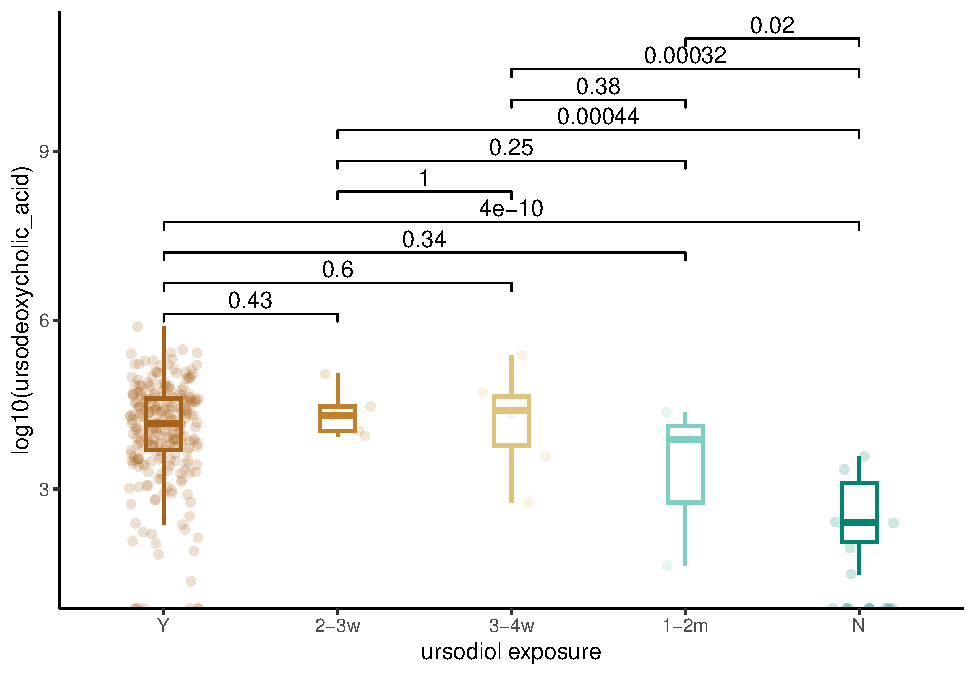
\includegraphics{_main_files/figure-latex/unnamed-chunk-5-1.pdf}

\hypertarget{plot-ursodiol-exposure-and-secondary-bas-concentrations}{%
\section{Plot ursodiol exposure and secondary BAs concentrations}\label{plot-ursodiol-exposure-and-secondary-bas-concentrations}}

\begin{Shaded}
\begin{Highlighting}[]
\NormalTok{both\_conc\_pools\_final }\SpecialCharTok{\%\textgreater{}\%} 
  \FunctionTok{ggplot}\NormalTok{(}\FunctionTok{aes}\NormalTok{(}\AttributeTok{x=}\NormalTok{ursodiol, }\AttributeTok{y=}\FunctionTok{log10}\NormalTok{(secondary\_pool), }\AttributeTok{color=}\NormalTok{ursodiol)) }\SpecialCharTok{+}
  \FunctionTok{geom\_boxplot}\NormalTok{(}\AttributeTok{width=}\FloatTok{0.2}\NormalTok{, }\AttributeTok{outlier.shape =}\ConstantTok{NA}\NormalTok{, }\AttributeTok{lwd=}\NormalTok{.}\DecValTok{7}\NormalTok{)}\SpecialCharTok{+}
  \FunctionTok{geom\_jitter}\NormalTok{(}\AttributeTok{width=}\FloatTok{0.2}\NormalTok{, }\AttributeTok{alpha=}\FloatTok{0.2}\NormalTok{)}\SpecialCharTok{+}
  \FunctionTok{theme\_classic}\NormalTok{() }\SpecialCharTok{+}
  \FunctionTok{xlab}\NormalTok{(}\StringTok{"ursodiol exposure"}\NormalTok{)}\SpecialCharTok{+}
  \FunctionTok{stat\_compare\_means}\NormalTok{(}\AttributeTok{comparisons=}\FunctionTok{list}\NormalTok{( }\FunctionTok{c}\NormalTok{(}\StringTok{"Y"}\NormalTok{, }\StringTok{"2{-}3w"}\NormalTok{),}\FunctionTok{c}\NormalTok{(}\StringTok{"3{-}4w"}\NormalTok{, }\StringTok{"Y"}\NormalTok{), }\FunctionTok{c}\NormalTok{(}\StringTok{"Y"}\NormalTok{, }\StringTok{"1{-}2m"}\NormalTok{), }\FunctionTok{c}\NormalTok{(}\StringTok{"N"}\NormalTok{, }\StringTok{"Y"}\NormalTok{),}
                                       \FunctionTok{c}\NormalTok{(}\StringTok{"3{-}4w"}\NormalTok{, }\StringTok{"2{-}3w"}\NormalTok{),}\FunctionTok{c}\NormalTok{(}\StringTok{"1{-}2m"}\NormalTok{, }\StringTok{"2{-}3w"}\NormalTok{), }\FunctionTok{c}\NormalTok{(}\StringTok{"N"}\NormalTok{, }\StringTok{"2{-}3w"}\NormalTok{),}
                                       \FunctionTok{c}\NormalTok{(}\StringTok{"1{-}2m"}\NormalTok{, }\StringTok{"3{-}4w"}\NormalTok{),  }\FunctionTok{c}\NormalTok{(}\StringTok{"N"}\NormalTok{, }\StringTok{"3{-}4w"}\NormalTok{),}
                                       \FunctionTok{c}\NormalTok{(}\StringTok{"N"}\NormalTok{, }\StringTok{"1{-}2m"}\NormalTok{)}
\NormalTok{  ),}
  \CommentTok{\#label="p.signif",}
  \AttributeTok{method=}\StringTok{"wilcox.test"}\NormalTok{,}
  \AttributeTok{correct=}\ConstantTok{FALSE}\NormalTok{)}\SpecialCharTok{+}
  \FunctionTok{scale\_color\_manual}\NormalTok{(}\AttributeTok{values=}\FunctionTok{c}\NormalTok{(}\StringTok{"\#a6611a"}\NormalTok{, }\StringTok{"\#bf812d"}\NormalTok{,}\StringTok{"\#dfc27d"}\NormalTok{, }\StringTok{"\#80cdc1"}\NormalTok{, }\StringTok{"\#018571"}\NormalTok{))}\SpecialCharTok{+}
  \FunctionTok{theme}\NormalTok{(}\AttributeTok{legend.position=}\StringTok{"none"}\NormalTok{)}
\end{Highlighting}
\end{Shaded}

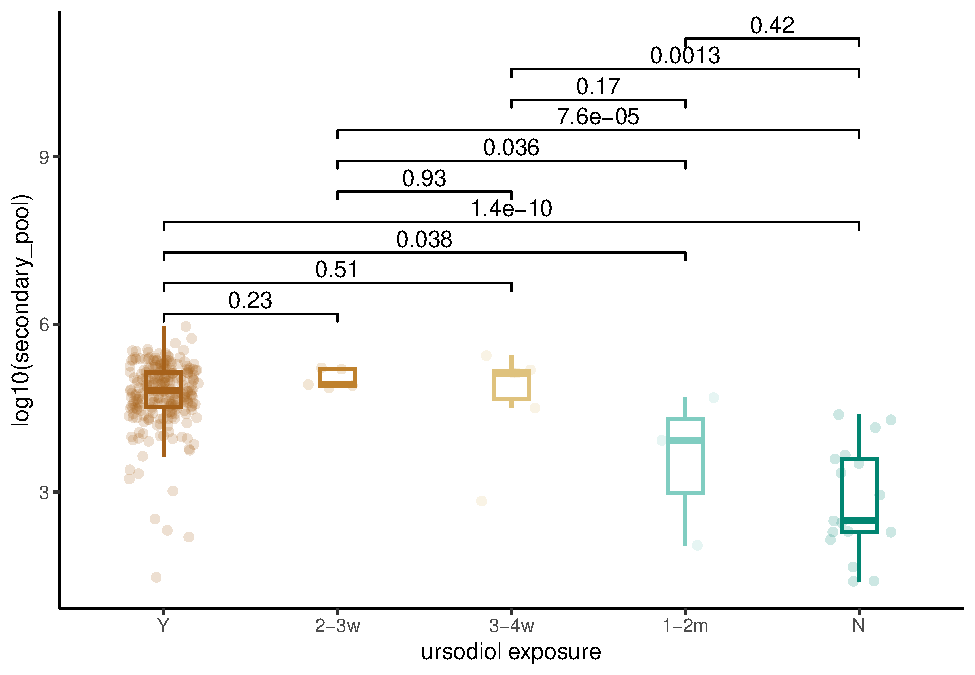
\includegraphics{_main_files/figure-latex/unnamed-chunk-6-1.pdf}

\hypertarget{plot-correlation-of-ursodiol-with-other-bile-acid-pools-plot-conjugated-udca-tauroursodeoxycholic_acidglycoursodeoxycholic_acid-tbas-total_bas-pbas-primary_pool-sbas-secondary_pool-nonudca-total-bas-total_nonudca_pool-nonudca-sbas-secondary_nonudca-secondaryprimary-ratio-sp_ratio}{%
\section{Plot correlation of ursodiol with other bile acid pools: plot conjugated UDCA (tauroursodeoxycholic\_acid+glycoursodeoxycholic\_acid), TBAs (total\_BAs), PBAs (primary\_pool), SBAs (secondary\_pool), nonUDCA total BAs (total\_nonUDCA\_pool), nonUDCA SBAs (secondary\_nonUDCA), secondary/primary ratio (SP\_ratio)}\label{plot-correlation-of-ursodiol-with-other-bile-acid-pools-plot-conjugated-udca-tauroursodeoxycholic_acidglycoursodeoxycholic_acid-tbas-total_bas-pbas-primary_pool-sbas-secondary_pool-nonudca-total-bas-total_nonudca_pool-nonudca-sbas-secondary_nonudca-secondaryprimary-ratio-sp_ratio}}

\begin{Shaded}
\begin{Highlighting}[]
\NormalTok{both\_conc\_pools\_final }\SpecialCharTok{\%\textgreater{}\%} 
  \FunctionTok{mutate}\NormalTok{(}\AttributeTok{SP\_ratio=}\NormalTok{secondary\_pool}\SpecialCharTok{/}\NormalTok{primary\_pool) }\SpecialCharTok{\%\textgreater{}\%} 
  \FunctionTok{mutate}\NormalTok{(}\AttributeTok{SP\_ratio\_nonUDCA=}\NormalTok{secondary\_nonUDCA}\SpecialCharTok{/}\NormalTok{primary\_pool) }\SpecialCharTok{\%\textgreater{}\%} 
  \FunctionTok{left\_join}\NormalTok{(both\_conc }\SpecialCharTok{\%\textgreater{}\%} \FunctionTok{select}\NormalTok{(sampleid, glycoursodeoxycholic\_acid, tauroursodeoxycholic\_acid, ursodeoxycholic\_acid)) }\SpecialCharTok{\%\textgreater{}\%} 
  \FunctionTok{ggplot}\NormalTok{(}\FunctionTok{aes}\NormalTok{(}\AttributeTok{y=}\FunctionTok{log10}\NormalTok{(}\StringTok{\textasciigrave{}}\AttributeTok{ursodeoxycholic\_acid}\StringTok{\textasciigrave{}}\SpecialCharTok{+}\FloatTok{2.5}\NormalTok{), }\AttributeTok{x=}\FunctionTok{log10}\NormalTok{(secondary\_pool}\FloatTok{+2.5}\NormalTok{)))}\SpecialCharTok{+}
  \FunctionTok{geom\_point}\NormalTok{(}\AttributeTok{size=}\FloatTok{0.8}\NormalTok{, }\AttributeTok{alpha=}\FloatTok{0.4}\NormalTok{)}\SpecialCharTok{+}
  \FunctionTok{geom\_smooth}\NormalTok{(}\AttributeTok{method=}\StringTok{"lm"}\NormalTok{)}\SpecialCharTok{+}
  \FunctionTok{stat\_cor}\NormalTok{(}\AttributeTok{method =} \StringTok{"pearson"}\NormalTok{)}\SpecialCharTok{+}
  \CommentTok{\#ylab("log10(UDCA)")+}
  \CommentTok{\#xlab("log10(PS\_nonUDCA)")+}
  \FunctionTok{theme\_classic}\NormalTok{()}
\end{Highlighting}
\end{Shaded}

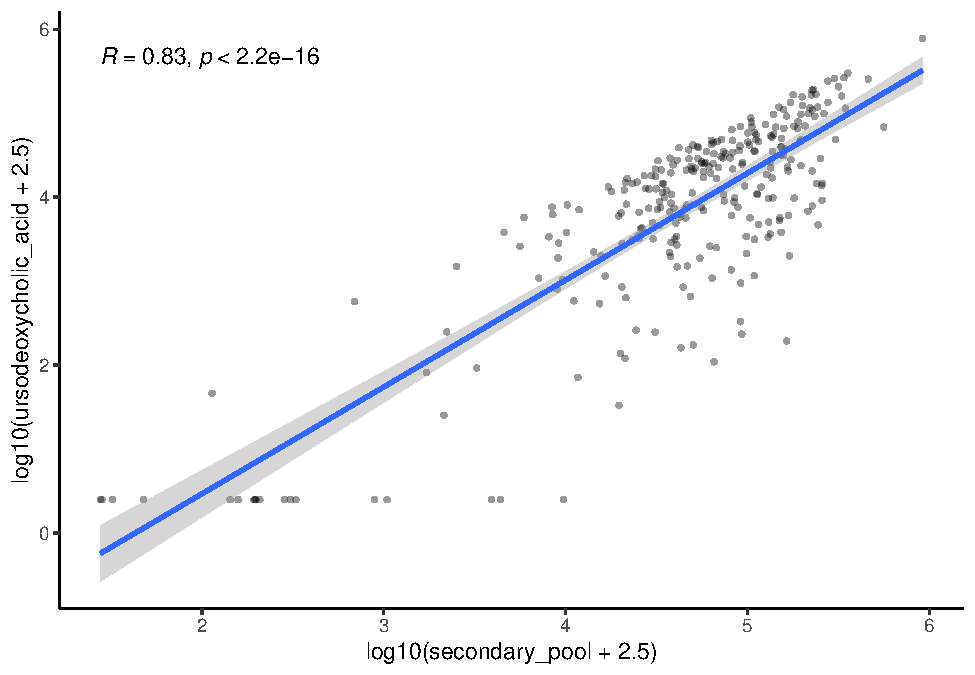
\includegraphics{_main_files/figure-latex/unnamed-chunk-7-1.pdf}

\hypertarget{create-correlation-plots-to-evaluate-association-of-udca-with-all-individual-bas}{%
\section{Create correlation plots to evaluate association of UDCA with all individual BAs}\label{create-correlation-plots-to-evaluate-association-of-udca-with-all-individual-bas}}

\begin{Shaded}
\begin{Highlighting}[]
\FunctionTok{library}\NormalTok{(corrplot)}

\NormalTok{precor\_data}\OtherTok{\textless{}{-}}\NormalTok{ filtered\_combined\_table }\SpecialCharTok{\%\textgreater{}\%} 
  \FunctionTok{column\_to\_rownames}\NormalTok{(}\StringTok{"sampleid"}\NormalTok{)}
\NormalTok{cor\_data}\OtherTok{\textless{}{-}}\FunctionTok{cor}\NormalTok{(precor\_data, }\AttributeTok{use =} \StringTok{"complete.obs"}\NormalTok{)}

\FunctionTok{corrplot}\NormalTok{(cor\_data)}
\end{Highlighting}
\end{Shaded}

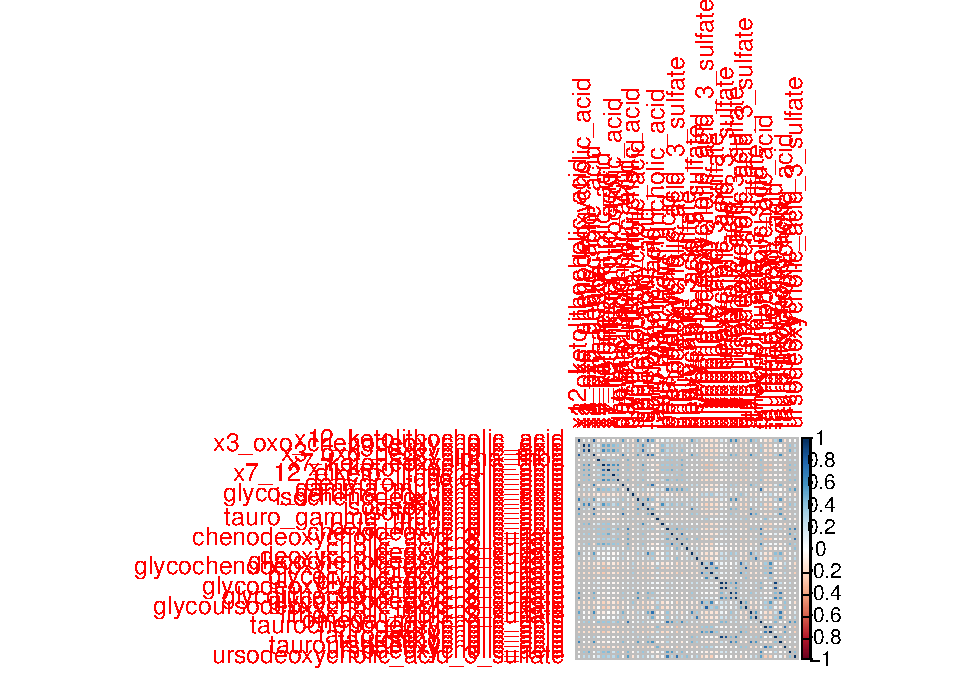
\includegraphics{_main_files/figure-latex/unnamed-chunk-8-1.pdf}

\hypertarget{visualization-of-significant-correlations-of-udca-with-individual-bas-r0.4}{%
\subsection{Visualization of significant correlations of UDCA with individual BAs (R\textgreater0.4)}\label{visualization-of-significant-correlations-of-udca-with-individual-bas-r0.4}}

\begin{Shaded}
\begin{Highlighting}[]
\NormalTok{precor\_data\_selected}\OtherTok{\textless{}{-}}\NormalTok{ filtered\_combined\_table }\SpecialCharTok{\%\textgreater{}\%} 
  \FunctionTok{column\_to\_rownames}\NormalTok{(}\StringTok{"sampleid"}\NormalTok{) }\SpecialCharTok{\%\textgreater{}\%} 
  \FunctionTok{select}\NormalTok{(ursodeoxycholic\_acid, ursocholic\_acid, beta\_muricholic\_acid, ursodeoxycholic\_acid\_3\_sulfate, x7\_ketodeoxycholic\_acid, }
\NormalTok{         x7\_ketolithocholic\_acid, gamma\_muricholic\_acid, cholic\_acid, chenodeoxycholic\_acid, x3\_oxo\_cholic\_acid)}

\NormalTok{cor\_data\_selected}\OtherTok{\textless{}{-}}\FunctionTok{cor}\NormalTok{(precor\_data\_selected, }\AttributeTok{use =} \StringTok{"complete.obs"}\NormalTok{)}

\FunctionTok{corrplot}\NormalTok{(cor\_data\_selected, }\AttributeTok{method =} \StringTok{"number"}\NormalTok{, }\AttributeTok{type =} \StringTok{"upper"}\NormalTok{)}
\end{Highlighting}
\end{Shaded}

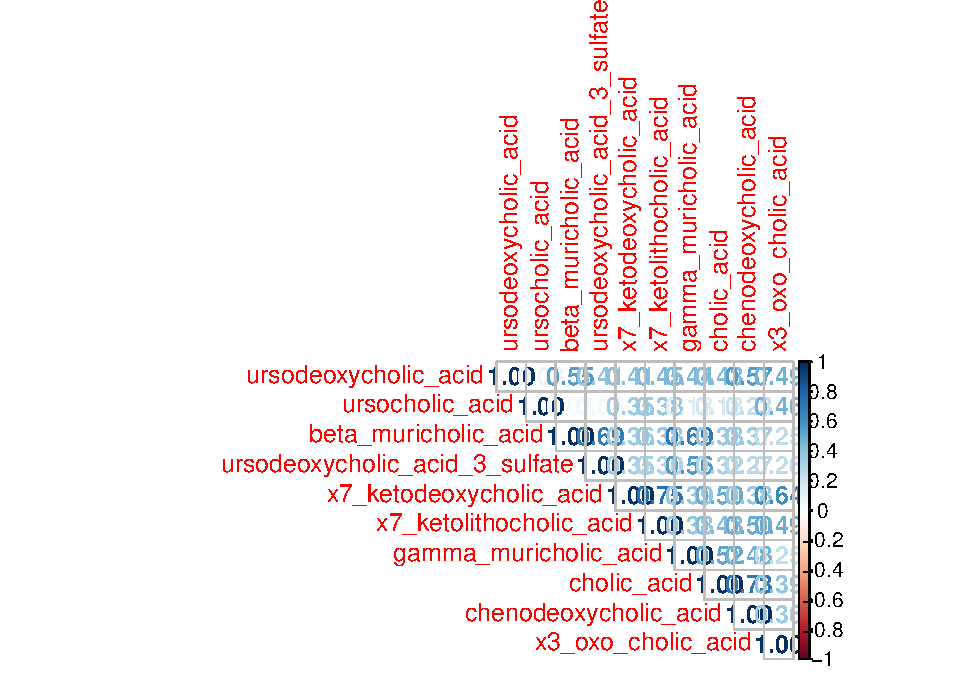
\includegraphics{_main_files/figure-latex/unnamed-chunk-9-1.pdf}

\hypertarget{create-the-bile-acid-pools-figure-4-supplementary-figure-68}{%
\chapter{Create the bile acid pools (figure 4, supplementary figure 6,8)}\label{create-the-bile-acid-pools-figure-4-supplementary-figure-68}}

\hypertarget{create-ba-pools-first-for-peri-gvhd-onset-timepoint}{%
\section{Create BA pools first for peri-GVHD-onset timepoint}\label{create-ba-pools-first-for-peri-gvhd-onset-timepoint}}

\begin{Shaded}
\begin{Highlighting}[]
\NormalTok{later}\OtherTok{\textless{}{-}}\NormalTok{ cohort\_BAS }\SpecialCharTok{\%\textgreater{}\%}\FunctionTok{filter}\NormalTok{(later}\SpecialCharTok{==}\StringTok{"Y"}\NormalTok{) }\SpecialCharTok{\%\textgreater{}\%} 
  \FunctionTok{filter}\NormalTok{(ursodiol}\SpecialCharTok{==}\StringTok{"Y"}\NormalTok{) }\SpecialCharTok{\%\textgreater{}\%} 
  \FunctionTok{select}\NormalTok{(sampleid, GI\_GVHD) }\SpecialCharTok{\%\textgreater{}\%} 
  \FunctionTok{left\_join}\NormalTok{(conc\_all\_filtered)}

\CommentTok{\#prep dataset prepping each BA depending on its classifications}
\NormalTok{later\_pools}\OtherTok{\textless{}{-}}\NormalTok{later }\SpecialCharTok{\%\textgreater{}\%} 
  \FunctionTok{gather}\NormalTok{(}\StringTok{"bile\_acid"}\NormalTok{, }\StringTok{"value"}\NormalTok{, }\FunctionTok{names}\NormalTok{(.)[}\DecValTok{5}\NormalTok{]}\SpecialCharTok{:}\FunctionTok{names}\NormalTok{(.)[}\FunctionTok{ncol}\NormalTok{(.)]) }\SpecialCharTok{\%\textgreater{}\%} 
  \FunctionTok{left\_join}\NormalTok{(ba\_families) }\SpecialCharTok{\%\textgreater{}\%} 
  \FunctionTok{mutate}\NormalTok{(}\AttributeTok{primary\_pool=}\FunctionTok{ifelse}\NormalTok{(prim\_vs\_sec}\SpecialCharTok{==}\StringTok{"Primary"}\NormalTok{, value, }\DecValTok{0}\NormalTok{)) }\SpecialCharTok{\%\textgreater{}\%} 
  \FunctionTok{mutate}\NormalTok{(}\AttributeTok{secondary\_pool=}\FunctionTok{ifelse}\NormalTok{(prim\_vs\_sec}\SpecialCharTok{==}\StringTok{"Secondary"}\NormalTok{, value, }\DecValTok{0}\NormalTok{)) }\SpecialCharTok{\%\textgreater{}\%} 
  \FunctionTok{mutate}\NormalTok{(}\AttributeTok{sulfated\_pool=}\FunctionTok{ifelse}\NormalTok{(sulfated}\SpecialCharTok{==}\StringTok{"Y"}\NormalTok{, value, }\DecValTok{0}\NormalTok{)) }\SpecialCharTok{\%\textgreater{}\%} 
  \FunctionTok{mutate}\NormalTok{(}\AttributeTok{conjugated\_pool=}\FunctionTok{ifelse}\NormalTok{(amidated}\SpecialCharTok{==}\StringTok{"Y"} \SpecialCharTok{\&}\NormalTok{ sulfated}\SpecialCharTok{==}\StringTok{"N"}\NormalTok{, value, }\DecValTok{0}\NormalTok{)) }\SpecialCharTok{\%\textgreater{}\%} 
  \FunctionTok{mutate}\NormalTok{(}\AttributeTok{unconjugated\_pool=}\FunctionTok{ifelse}\NormalTok{(amidated}\SpecialCharTok{==}\StringTok{"N"} \SpecialCharTok{\&}\NormalTok{ sulfated}\SpecialCharTok{==}\StringTok{"N"}\NormalTok{, value, }\DecValTok{0}\NormalTok{)) }\SpecialCharTok{\%\textgreater{}\%} 
  \FunctionTok{mutate}\NormalTok{(}\AttributeTok{secondary\_nonUDCA=}\FunctionTok{ifelse}\NormalTok{(prim\_vs\_sec}\SpecialCharTok{==}\StringTok{"Secondary"} \SpecialCharTok{\&}\NormalTok{ udca}\SpecialCharTok{==}\StringTok{"N"}\NormalTok{, value, }\DecValTok{0}\NormalTok{)) }\SpecialCharTok{\%\textgreater{}\%} 
  \FunctionTok{mutate}\NormalTok{(}\AttributeTok{total\_BAs=}\NormalTok{value) }\SpecialCharTok{\%\textgreater{}\%} 
  \FunctionTok{mutate}\NormalTok{(}\AttributeTok{total\_nonUDCA\_pool=}\FunctionTok{ifelse}\NormalTok{(udca}\SpecialCharTok{==}\StringTok{"N"}\NormalTok{, value, }\DecValTok{0}\NormalTok{)) }\SpecialCharTok{\%\textgreater{}\%} 
  \FunctionTok{mutate}\NormalTok{(}\AttributeTok{glycine\_pool=}\FunctionTok{ifelse}\NormalTok{(glycine}\SpecialCharTok{==}\StringTok{"Y"} \SpecialCharTok{\&}\NormalTok{ sulfated}\SpecialCharTok{==}\StringTok{"N"}\NormalTok{, value, }\DecValTok{0}\NormalTok{)) }\SpecialCharTok{\%\textgreater{}\%} 
  \FunctionTok{mutate}\NormalTok{(}\AttributeTok{taurine\_pool=}\FunctionTok{ifelse}\NormalTok{(taurine}\SpecialCharTok{==}\StringTok{"Y"} \SpecialCharTok{\&}\NormalTok{ sulfated}\SpecialCharTok{==}\StringTok{"N"}\NormalTok{, value, }\DecValTok{0}\NormalTok{)) }\SpecialCharTok{\%\textgreater{}\%} 
  \FunctionTok{mutate}\NormalTok{(}\AttributeTok{taurine\_SBA\_pool=}\FunctionTok{ifelse}\NormalTok{(taurine}\SpecialCharTok{==}\StringTok{"Y"} \SpecialCharTok{\&}\NormalTok{ prim\_vs\_sec}\SpecialCharTok{==}\StringTok{"Secondary"} \SpecialCharTok{\&}\NormalTok{ sulfated}\SpecialCharTok{==}\StringTok{"N"}\NormalTok{, value, }\DecValTok{0}\NormalTok{)) }\SpecialCharTok{\%\textgreater{}\%} 
  \FunctionTok{mutate}\NormalTok{(}\AttributeTok{taurine\_PBA\_pool=}\FunctionTok{ifelse}\NormalTok{(taurine}\SpecialCharTok{==}\StringTok{"Y"} \SpecialCharTok{\&}\NormalTok{ prim\_vs\_sec}\SpecialCharTok{==}\StringTok{"Primary"} \SpecialCharTok{\&}\NormalTok{ sulfated}\SpecialCharTok{==}\StringTok{"N"}\NormalTok{, value, }\DecValTok{0}\NormalTok{)) }\SpecialCharTok{\%\textgreater{}\%} 
  \FunctionTok{mutate}\NormalTok{(}\AttributeTok{glycine\_SBA\_pool=}\FunctionTok{ifelse}\NormalTok{(glycine}\SpecialCharTok{==}\StringTok{"Y"}\SpecialCharTok{\&}\NormalTok{ prim\_vs\_sec}\SpecialCharTok{==}\StringTok{"Secondary"} \SpecialCharTok{\&}\NormalTok{ sulfated}\SpecialCharTok{==}\StringTok{"N"}\NormalTok{, value, }\DecValTok{0}\NormalTok{)) }\SpecialCharTok{\%\textgreater{}\%} 
  \FunctionTok{mutate}\NormalTok{(}\AttributeTok{glycine\_PBA\_pool=}\FunctionTok{ifelse}\NormalTok{(glycine}\SpecialCharTok{==}\StringTok{"Y"} \SpecialCharTok{\&}\NormalTok{prim\_vs\_sec}\SpecialCharTok{==}\StringTok{"Primary"}\SpecialCharTok{\&}\NormalTok{ sulfated}\SpecialCharTok{==}\StringTok{"N"}\NormalTok{, value, }\DecValTok{0}\NormalTok{)) }\SpecialCharTok{\%\textgreater{}\%} 
  \FunctionTok{select}\NormalTok{(}\SpecialCharTok{{-}}\FunctionTok{colnames}\NormalTok{(ba\_families), }\SpecialCharTok{{-}}\NormalTok{value) }

\CommentTok{\#replace NAs with 0 to be able to add sums}
\NormalTok{later\_pools[}\FunctionTok{is.na}\NormalTok{(later\_pools)]}\OtherTok{\textless{}{-}}\DecValTok{0}

\NormalTok{later\_pools\_final}\OtherTok{\textless{}{-}}\NormalTok{later\_pools }\SpecialCharTok{\%\textgreater{}\%} 
  \CommentTok{\#gather("bile\_acid", "value", names(.)[2]:names(.)[ncol(.)]) \%\textgreater{}\% }
  \CommentTok{\#summarise(sum\_group=sum(value))}
  \FunctionTok{group\_by}\NormalTok{(sampleid) }\SpecialCharTok{\%\textgreater{}\%} 
  \FunctionTok{summarise}\NormalTok{(}\FunctionTok{across}\NormalTok{(}\FunctionTok{where}\NormalTok{(is.numeric), sum))}
\end{Highlighting}
\end{Shaded}

\hypertarget{plot-tbas-total_bas-pbas-primary_pool-sbas-secondary_pool-nonudca-sbas-secondary_nonudca-conjugated-conjugated_pool-unconjugated-unconjugated_pool-sulfated-sulfated_pool}{%
\subsection{Plot: TBAs (total\_BAs), PBAs (primary\_pool), SBAs (secondary\_pool), nonUDCA SBAs (secondary\_nonUDCA), conjugated (conjugated\_pool), unconjugated (unconjugated\_pool), sulfated (sulfated\_pool)}\label{plot-tbas-total_bas-pbas-primary_pool-sbas-secondary_pool-nonudca-sbas-secondary_nonudca-conjugated-conjugated_pool-unconjugated-unconjugated_pool-sulfated-sulfated_pool}}

\begin{Shaded}
\begin{Highlighting}[]
\NormalTok{later\_pools\_final }\SpecialCharTok{\%\textgreater{}\%} 
  \FunctionTok{left\_join}\NormalTok{(cohort\_BAS) }\SpecialCharTok{\%\textgreater{}\%}
  \FunctionTok{mutate}\NormalTok{(}\AttributeTok{GI\_GVHD=}\FunctionTok{ifelse}\NormalTok{(GI\_GVHD}\SpecialCharTok{==}\StringTok{"Y"}\NormalTok{, }\StringTok{"GVHD"}\NormalTok{, }\StringTok{"CTRL"}\NormalTok{)) }\SpecialCharTok{\%\textgreater{}\%} 
  \FunctionTok{mutate}\NormalTok{(}\AttributeTok{sp\_ratio=}\NormalTok{secondary\_pool}\SpecialCharTok{/}\NormalTok{primary\_pool) }\SpecialCharTok{\%\textgreater{}\%} 
  \FunctionTok{mutate}\NormalTok{(}\AttributeTok{sp\_nonUDCA\_ratio=}\NormalTok{secondary\_nonUDCA}\SpecialCharTok{/}\NormalTok{primary\_pool) }\SpecialCharTok{\%\textgreater{}\%} 
  \FunctionTok{mutate}\NormalTok{(}\AttributeTok{unconj\_conj=}\NormalTok{unconjugated\_pool}\SpecialCharTok{/}\NormalTok{conjugated\_pool) }\SpecialCharTok{\%\textgreater{}\%} 
  \FunctionTok{ggplot}\NormalTok{(}\FunctionTok{aes}\NormalTok{(}\AttributeTok{x=}\NormalTok{GI\_GVHD, }\AttributeTok{y=}\FunctionTok{log10}\NormalTok{(unconj\_conj), }\AttributeTok{colour=}\NormalTok{GI\_GVHD))}\SpecialCharTok{+}
  \FunctionTok{geom\_boxplot}\NormalTok{(}\AttributeTok{width=}\FloatTok{0.2}\NormalTok{, }\AttributeTok{lwd=}\FloatTok{0.8}\NormalTok{, }\AttributeTok{outlier.shape =} \ConstantTok{NA}\NormalTok{) }\SpecialCharTok{+}
  \FunctionTok{geom\_jitter}\NormalTok{(}\AttributeTok{width=}\FloatTok{0.3}\NormalTok{, }\AttributeTok{alpha=}\FloatTok{0.3}\NormalTok{, }\AttributeTok{size=}\FloatTok{2.5}\NormalTok{)}\SpecialCharTok{+}
  \FunctionTok{ylab}\NormalTok{(}\StringTok{"log10(unconj\_conj)"}\NormalTok{)}\SpecialCharTok{+}
  \FunctionTok{xlab}\NormalTok{(}\StringTok{""}\NormalTok{)}\SpecialCharTok{+}
  \FunctionTok{theme\_classic}\NormalTok{()}\SpecialCharTok{+}
  \FunctionTok{stat\_compare\_means}\NormalTok{(}\AttributeTok{comparisons=}\FunctionTok{list}\NormalTok{(}\FunctionTok{c}\NormalTok{(}\StringTok{"CTRL"}\NormalTok{, }\StringTok{"GVHD"}\NormalTok{)),}
                     \AttributeTok{method=}\StringTok{"wilcox.test"}\NormalTok{,}
                     \AttributeTok{correct=}\ConstantTok{FALSE}\NormalTok{)}\SpecialCharTok{+}
  \FunctionTok{scale\_color\_manual}\NormalTok{(}\AttributeTok{values=}\FunctionTok{c}\NormalTok{(}\StringTok{"dodgerblue4"}\NormalTok{, }\StringTok{"red3"}\NormalTok{))}\SpecialCharTok{+}
  \FunctionTok{theme}\NormalTok{(}\AttributeTok{legend.position=}\StringTok{"none"}\NormalTok{)}
\end{Highlighting}
\end{Shaded}

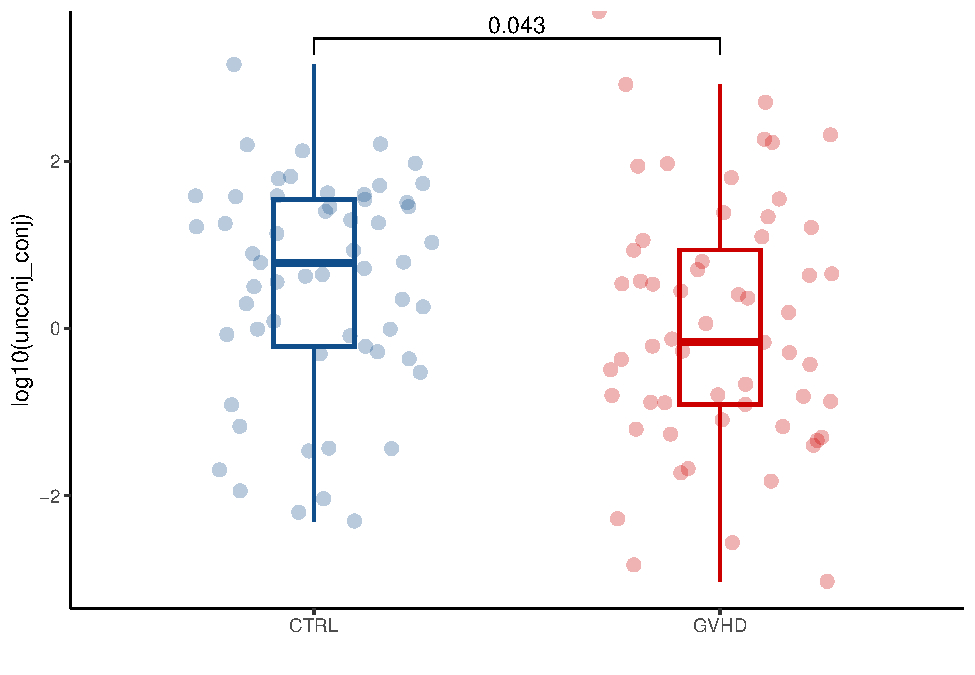
\includegraphics{_main_files/figure-latex/unnamed-chunk-11-1.pdf}

\hypertarget{create-pies}{%
\subsection{Create pies}\label{create-pies}}

\begin{Shaded}
\begin{Highlighting}[]
\NormalTok{dataset\_pre}\OtherTok{\textless{}{-}}\NormalTok{later\_pools\_final }\SpecialCharTok{\%\textgreater{}\%} 
  \FunctionTok{gather}\NormalTok{(}\StringTok{"BA\_pool"}\NormalTok{, }\StringTok{"value"}\NormalTok{, }\FunctionTok{names}\NormalTok{(.)[}\DecValTok{2}\NormalTok{]}\SpecialCharTok{:}\FunctionTok{names}\NormalTok{(.)[}\FunctionTok{ncol}\NormalTok{(.)]) }\SpecialCharTok{\%\textgreater{}\%} 
  \FunctionTok{left\_join}\NormalTok{(cohort\_BAS }\SpecialCharTok{\%\textgreater{}\%} 
              \FunctionTok{select}\NormalTok{(sampleid, GI\_GVHD, later, ursodiol)) }\SpecialCharTok{\%\textgreater{}\%} 
  \FunctionTok{filter}\NormalTok{(later}\SpecialCharTok{==}\StringTok{"Y"}\NormalTok{) }\SpecialCharTok{\%\textgreater{}\%} 
  \FunctionTok{filter}\NormalTok{(ursodiol}\SpecialCharTok{==}\StringTok{"Y"}\NormalTok{) }\SpecialCharTok{\%\textgreater{}\%} 
  \FunctionTok{select}\NormalTok{(}\SpecialCharTok{{-}}\NormalTok{ursodiol, }\SpecialCharTok{{-}}\NormalTok{later) }\SpecialCharTok{\%\textgreater{}\%} 
  \FunctionTok{group\_by}\NormalTok{(GI\_GVHD, BA\_pool) }\SpecialCharTok{\%\textgreater{}\%} 
  \FunctionTok{summarise}\NormalTok{(}\AttributeTok{ave\_pool=}\FunctionTok{ave}\NormalTok{(value)) }\SpecialCharTok{\%\textgreater{}\%} \FunctionTok{slice}\NormalTok{(}\DecValTok{1}\NormalTok{)}
\end{Highlighting}
\end{Shaded}

\begin{verbatim}
## Joining with `by = join_by(sampleid)`
\end{verbatim}

\begin{verbatim}
## Warning: Returning more (or less) than 1 row per `summarise()` group was deprecated in
## dplyr 1.1.0.
## i Please use `reframe()` instead.
## i When switching from `summarise()` to `reframe()`, remember that `reframe()`
##   always returns an ungrouped data frame and adjust accordingly.
## Call `lifecycle::last_lifecycle_warnings()` to see where this warning was
## generated.
\end{verbatim}

\begin{verbatim}
## `summarise()` has grouped output by 'GI_GVHD', 'BA_pool'. You can override
## using the `.groups` argument.
\end{verbatim}

\begin{Shaded}
\begin{Highlighting}[]
\NormalTok{dataset\_pre2}\OtherTok{\textless{}{-}}\NormalTok{dataset\_pre }\SpecialCharTok{\%\textgreater{}\%} 
  \CommentTok{\#filter(BA\_pool=="primary\_pool"|BA\_pool=="secondary\_nonUDCA") \%\textgreater{}\% \#to evaluate nonUDCA secondary and primary polls}
  \CommentTok{\#filter(BA\_pool=="primary\_pool"|BA\_pool=="secondary\_pool") \%\textgreater{}\% \#to evaluate total secondary}
  \FunctionTok{filter}\NormalTok{(BA\_pool}\SpecialCharTok{==}\StringTok{"glycine\_pool"}\SpecialCharTok{|}\NormalTok{BA\_pool}\SpecialCharTok{==}\StringTok{"taurine\_pool"}\SpecialCharTok{|}\NormalTok{BA\_pool}\SpecialCharTok{==}\StringTok{"sulfated\_pool"}\SpecialCharTok{|}\NormalTok{BA\_pool}\SpecialCharTok{==}\StringTok{"unconjugated\_pool"}\NormalTok{) }\SpecialCharTok{\%\textgreater{}\%} 
  \FunctionTok{rename}\NormalTok{(}\AttributeTok{group=}\NormalTok{BA\_pool) }\SpecialCharTok{\%\textgreater{}\%} 
  \FunctionTok{rename}\NormalTok{(}\AttributeTok{value=}\NormalTok{ave\_pool) }\SpecialCharTok{\%\textgreater{}\%} 
  \FunctionTok{ungroup}\NormalTok{() }\SpecialCharTok{\%\textgreater{}\%} 
  \FunctionTok{group\_by}\NormalTok{(GI\_GVHD) }\SpecialCharTok{\%\textgreater{}\%} 
  \FunctionTok{mutate}\NormalTok{(}\AttributeTok{sum\_value=}\FunctionTok{sum}\NormalTok{(value)) }\SpecialCharTok{\%\textgreater{}\%} 
  \FunctionTok{mutate}\NormalTok{(}\AttributeTok{perc=}\NormalTok{value}\SpecialCharTok{/}\NormalTok{sum\_value) }\SpecialCharTok{\%\textgreater{}\%} 
  \FunctionTok{mutate}\NormalTok{(}\AttributeTok{labels =}\NormalTok{ scales}\SpecialCharTok{::}\FunctionTok{percent}\NormalTok{(perc)) }\SpecialCharTok{\%\textgreater{}\%} 
  \FunctionTok{ungroup}\NormalTok{()}

\CommentTok{\#only run below when evaluating glycine/taurine conjugation as wel}
\CommentTok{\#define order of piechart for glycine/taurin conjugation}
\NormalTok{dataset\_pre2}\SpecialCharTok{$}\NormalTok{group }\OtherTok{\textless{}{-}} \FunctionTok{factor}\NormalTok{(dataset\_pre2}\SpecialCharTok{$}\NormalTok{group, }\AttributeTok{levels =} \FunctionTok{c}\NormalTok{(}\StringTok{"glycine\_pool"}\NormalTok{, }\StringTok{"taurine\_pool"}\NormalTok{,}\StringTok{"unconjugated\_pool"}\NormalTok{,}\StringTok{"sulfated\_pool"}\NormalTok{))}


\NormalTok{cp}\OtherTok{\textless{}{-}}\FunctionTok{coord\_polar}\NormalTok{(}\AttributeTok{theta=}\StringTok{"y"}\NormalTok{)}
\NormalTok{cp}\SpecialCharTok{$}\NormalTok{is\_free}\OtherTok{\textless{}{-}}\ControlFlowTok{function}\NormalTok{()}\ConstantTok{TRUE}

\FunctionTok{ggplot}\NormalTok{(dataset\_pre2, }\FunctionTok{aes}\NormalTok{(}\AttributeTok{x=}\StringTok{""}\NormalTok{, }\AttributeTok{y=}\NormalTok{perc, }\AttributeTok{fill=}\NormalTok{group))}\SpecialCharTok{+}
  \FunctionTok{geom\_bar}\NormalTok{(}\AttributeTok{stat=}\StringTok{"identity"}\NormalTok{, }\AttributeTok{width=}\DecValTok{1}\NormalTok{)}\SpecialCharTok{+}\NormalTok{cp}\SpecialCharTok{+}
  \FunctionTok{facet\_wrap}\NormalTok{(.}\SpecialCharTok{\textasciitilde{}}\NormalTok{GI\_GVHD, }\AttributeTok{scales=}\StringTok{"free"}\NormalTok{)}\SpecialCharTok{+}
  \FunctionTok{geom\_text}\NormalTok{(}\FunctionTok{aes}\NormalTok{(}\AttributeTok{label =}\NormalTok{ labels),}
            \AttributeTok{position =} \FunctionTok{position\_stack}\NormalTok{(}\AttributeTok{vjust =} \FloatTok{0.5}\NormalTok{)) }\SpecialCharTok{+}
  \FunctionTok{theme\_void}\NormalTok{()}\SpecialCharTok{+}
  \FunctionTok{theme}\NormalTok{(}\AttributeTok{axis.ticks=}\FunctionTok{element\_blank}\NormalTok{(),}
        \AttributeTok{axis.title=}\FunctionTok{element\_blank}\NormalTok{(),}
        \AttributeTok{axis.text.y=}\FunctionTok{element\_blank}\NormalTok{())}\SpecialCharTok{+}
  \FunctionTok{scale\_fill\_manual}\NormalTok{(}\AttributeTok{values=}\FunctionTok{c}\NormalTok{(}\StringTok{"green4"}\NormalTok{,}\StringTok{"chartreuse3"}\NormalTok{,}\StringTok{"dodgerblue2"}\NormalTok{,}\StringTok{"purple2"}\NormalTok{)) }\CommentTok{\#to evaluated amidation/sulfation}
\end{Highlighting}
\end{Shaded}

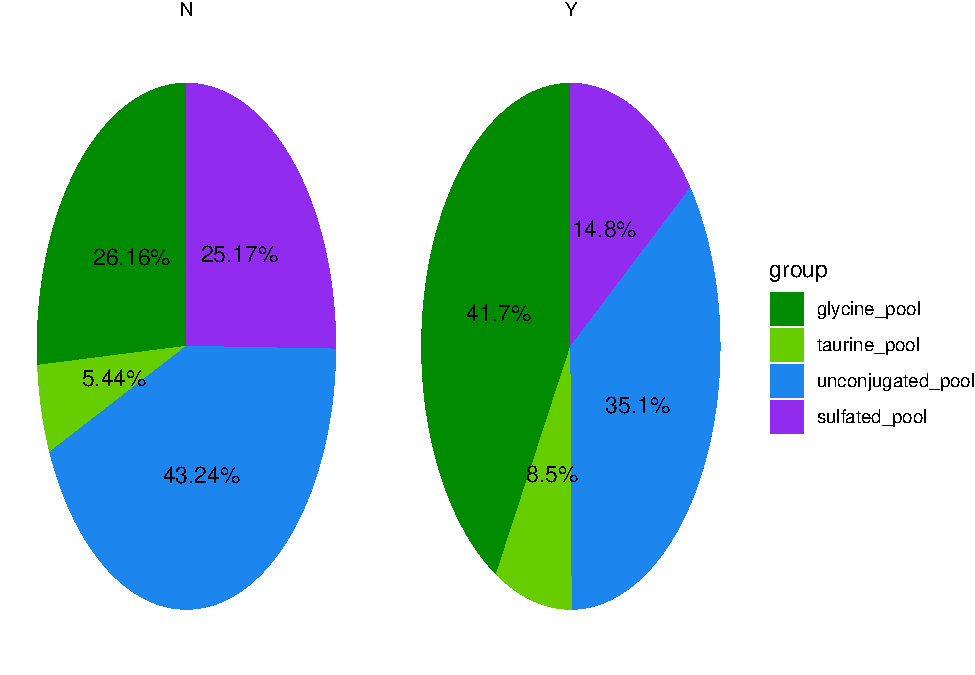
\includegraphics{_main_files/figure-latex/unnamed-chunk-12-1.pdf}

\hypertarget{create-ba-pools-for-peri-engraftment-timepoint}{%
\section{Create BA pools for peri-engraftment timepoint}\label{create-ba-pools-for-peri-engraftment-timepoint}}

\begin{Shaded}
\begin{Highlighting}[]
\NormalTok{periengr\_conc}\OtherTok{\textless{}{-}}\NormalTok{ cohort\_BAS }\SpecialCharTok{\%\textgreater{}\%}\FunctionTok{filter}\NormalTok{(periengr}\SpecialCharTok{==}\StringTok{"Y"}\NormalTok{) }\SpecialCharTok{\%\textgreater{}\%} 
  \FunctionTok{filter}\NormalTok{(ursodiol}\SpecialCharTok{==}\StringTok{"Y"}\NormalTok{) }\SpecialCharTok{\%\textgreater{}\%} 
  \FunctionTok{select}\NormalTok{(sampleid, GI\_GVHD) }\SpecialCharTok{\%\textgreater{}\%} 
  \FunctionTok{left\_join}\NormalTok{(conc\_all\_filtered) }\SpecialCharTok{\%\textgreater{}\%} 
  \FunctionTok{select}\NormalTok{(}\SpecialCharTok{{-}}\StringTok{\textasciigrave{}}\AttributeTok{beta\_muricholic\_acid}\StringTok{\textasciigrave{}}\NormalTok{, }\SpecialCharTok{{-}}\StringTok{\textasciigrave{}}\AttributeTok{omega\_muricholic\_acid}\StringTok{\textasciigrave{}}\NormalTok{) }\CommentTok{\#remove since it is not measured in all samples}

\CommentTok{\#prep dataset prepping each BA depending on its classifications}
\NormalTok{periengr\_pools}\OtherTok{\textless{}{-}}\NormalTok{periengr\_conc }\SpecialCharTok{\%\textgreater{}\%} 
  \FunctionTok{gather}\NormalTok{(}\StringTok{"bile\_acid"}\NormalTok{, }\StringTok{"value"}\NormalTok{, }\FunctionTok{names}\NormalTok{(.)[}\DecValTok{3}\NormalTok{]}\SpecialCharTok{:}\FunctionTok{names}\NormalTok{(.)[}\FunctionTok{ncol}\NormalTok{(.)]) }\SpecialCharTok{\%\textgreater{}\%} 
  \FunctionTok{left\_join}\NormalTok{(ba\_families) }\SpecialCharTok{\%\textgreater{}\%} 
  \FunctionTok{mutate}\NormalTok{(}\AttributeTok{primary\_pool=}\FunctionTok{ifelse}\NormalTok{(prim\_vs\_sec}\SpecialCharTok{==}\StringTok{"Primary"}\NormalTok{, value, }\DecValTok{0}\NormalTok{)) }\SpecialCharTok{\%\textgreater{}\%} 
  \FunctionTok{mutate}\NormalTok{(}\AttributeTok{secondary\_pool=}\FunctionTok{ifelse}\NormalTok{(prim\_vs\_sec}\SpecialCharTok{==}\StringTok{"Secondary"}\NormalTok{, value, }\DecValTok{0}\NormalTok{)) }\SpecialCharTok{\%\textgreater{}\%} 
  \FunctionTok{mutate}\NormalTok{(}\AttributeTok{sulfated\_pool=}\FunctionTok{ifelse}\NormalTok{(sulfated}\SpecialCharTok{==}\StringTok{"Y"}\NormalTok{, value, }\DecValTok{0}\NormalTok{)) }\SpecialCharTok{\%\textgreater{}\%} 
  \FunctionTok{mutate}\NormalTok{(}\AttributeTok{conjugated\_pool=}\FunctionTok{ifelse}\NormalTok{(amidated}\SpecialCharTok{==}\StringTok{"Y"} \SpecialCharTok{\&}\NormalTok{ sulfated}\SpecialCharTok{==}\StringTok{"N"}\NormalTok{, value, }\DecValTok{0}\NormalTok{)) }\SpecialCharTok{\%\textgreater{}\%} 
  \FunctionTok{mutate}\NormalTok{(}\AttributeTok{unconjugated\_pool=}\FunctionTok{ifelse}\NormalTok{(amidated}\SpecialCharTok{==}\StringTok{"N"} \SpecialCharTok{\&}\NormalTok{ sulfated}\SpecialCharTok{==}\StringTok{"N"}\NormalTok{, value, }\DecValTok{0}\NormalTok{)) }\SpecialCharTok{\%\textgreater{}\%} 
  \FunctionTok{mutate}\NormalTok{(}\AttributeTok{secondary\_nonUDCA=}\FunctionTok{ifelse}\NormalTok{(prim\_vs\_sec}\SpecialCharTok{==}\StringTok{"Secondary"} \SpecialCharTok{\&}\NormalTok{ udca}\SpecialCharTok{==}\StringTok{"N"}\NormalTok{, value, }\DecValTok{0}\NormalTok{)) }\SpecialCharTok{\%\textgreater{}\%} 
  \FunctionTok{mutate}\NormalTok{(}\AttributeTok{total\_BAs=}\NormalTok{value) }\SpecialCharTok{\%\textgreater{}\%} 
  \FunctionTok{mutate}\NormalTok{(}\AttributeTok{total\_nonUDCA\_pool=}\FunctionTok{ifelse}\NormalTok{(udca}\SpecialCharTok{==}\StringTok{"N"}\NormalTok{, value, }\DecValTok{0}\NormalTok{)) }\SpecialCharTok{\%\textgreater{}\%} 
  \FunctionTok{mutate}\NormalTok{(}\AttributeTok{glycine\_pool=}\FunctionTok{ifelse}\NormalTok{(glycine}\SpecialCharTok{==}\StringTok{"Y"} \SpecialCharTok{\&}\NormalTok{ sulfated}\SpecialCharTok{==}\StringTok{"N"}\NormalTok{, value, }\DecValTok{0}\NormalTok{)) }\SpecialCharTok{\%\textgreater{}\%} 
  \FunctionTok{mutate}\NormalTok{(}\AttributeTok{taurine\_pool=}\FunctionTok{ifelse}\NormalTok{(taurine}\SpecialCharTok{==}\StringTok{"Y"} \SpecialCharTok{\&}\NormalTok{ sulfated}\SpecialCharTok{==}\StringTok{"N"}\NormalTok{, value, }\DecValTok{0}\NormalTok{)) }\SpecialCharTok{\%\textgreater{}\%} 
  \FunctionTok{mutate}\NormalTok{(}\AttributeTok{taurine\_SBA\_pool=}\FunctionTok{ifelse}\NormalTok{(taurine}\SpecialCharTok{==}\StringTok{"Y"} \SpecialCharTok{\&}\NormalTok{ prim\_vs\_sec}\SpecialCharTok{==}\StringTok{"Secondary"} \SpecialCharTok{\&}\NormalTok{ sulfated}\SpecialCharTok{==}\StringTok{"N"}\NormalTok{, value, }\DecValTok{0}\NormalTok{)) }\SpecialCharTok{\%\textgreater{}\%} 
  \FunctionTok{mutate}\NormalTok{(}\AttributeTok{taurine\_PBA\_pool=}\FunctionTok{ifelse}\NormalTok{(taurine}\SpecialCharTok{==}\StringTok{"Y"} \SpecialCharTok{\&}\NormalTok{ prim\_vs\_sec}\SpecialCharTok{==}\StringTok{"Primary"} \SpecialCharTok{\&}\NormalTok{ sulfated}\SpecialCharTok{==}\StringTok{"N"}\NormalTok{, value, }\DecValTok{0}\NormalTok{)) }\SpecialCharTok{\%\textgreater{}\%} 
  \FunctionTok{mutate}\NormalTok{(}\AttributeTok{glycine\_SBA\_pool=}\FunctionTok{ifelse}\NormalTok{(glycine}\SpecialCharTok{==}\StringTok{"Y"}\SpecialCharTok{\&}\NormalTok{ prim\_vs\_sec}\SpecialCharTok{==}\StringTok{"Secondary"} \SpecialCharTok{\&}\NormalTok{ sulfated}\SpecialCharTok{==}\StringTok{"N"}\NormalTok{, value, }\DecValTok{0}\NormalTok{)) }\SpecialCharTok{\%\textgreater{}\%} 
  \FunctionTok{mutate}\NormalTok{(}\AttributeTok{glycine\_PBA\_pool=}\FunctionTok{ifelse}\NormalTok{(glycine}\SpecialCharTok{==}\StringTok{"Y"} \SpecialCharTok{\&}\NormalTok{prim\_vs\_sec}\SpecialCharTok{==}\StringTok{"Primary"}\SpecialCharTok{\&}\NormalTok{ sulfated}\SpecialCharTok{==}\StringTok{"N"}\NormalTok{, value, }\DecValTok{0}\NormalTok{)) }\SpecialCharTok{\%\textgreater{}\%} 
  \FunctionTok{select}\NormalTok{(}\SpecialCharTok{{-}}\FunctionTok{colnames}\NormalTok{(ba\_families), }\SpecialCharTok{{-}}\NormalTok{value) }
  
\CommentTok{\#replace NAs with 0 to be able to add sums}
\NormalTok{periengr\_pools[}\FunctionTok{is.na}\NormalTok{(periengr\_pools)]}\OtherTok{\textless{}{-}}\DecValTok{0}

\CommentTok{\#final table with each group sum}
\NormalTok{periengr\_pools\_final}\OtherTok{\textless{}{-}}\NormalTok{periengr\_pools }\SpecialCharTok{\%\textgreater{}\%} 
  \FunctionTok{group\_by}\NormalTok{(sampleid) }\SpecialCharTok{\%\textgreater{}\%} 
  \FunctionTok{summarise}\NormalTok{(}\FunctionTok{across}\NormalTok{(}\FunctionTok{where}\NormalTok{(is.numeric), sum))}
\end{Highlighting}
\end{Shaded}

\hypertarget{plot-ba-pools-and-gvhd-can-plot-total-bas-total_bas-pbas-primary_pool-sbas-secondary_pool-nonudca-sbas-secondary_nonudca-conjugated-conjugated_pool-unconjugated-unconjugated_pool-sulfated_pool-secondaryprimary-ratio-and-secondaryprimary-ratio}{%
\subsection{Plot BA pools and GVHD; can plot total BAs (total\_BAs), PBAs (primary\_pool), SBAs (secondary\_pool), nonUDCA SBAs (secondary\_nonUDCA), conjugated (conjugated\_pool), unconjugated (unconjugated\_pool), sulfated\_pool, secondary/primary ratio and secondary*/primary ratio}\label{plot-ba-pools-and-gvhd-can-plot-total-bas-total_bas-pbas-primary_pool-sbas-secondary_pool-nonudca-sbas-secondary_nonudca-conjugated-conjugated_pool-unconjugated-unconjugated_pool-sulfated_pool-secondaryprimary-ratio-and-secondaryprimary-ratio}}

\begin{Shaded}
\begin{Highlighting}[]
\NormalTok{periengr\_pools\_final }\SpecialCharTok{\%\textgreater{}\%} 
  \FunctionTok{left\_join}\NormalTok{(cohort\_BAS) }\SpecialCharTok{\%\textgreater{}\%}
  \FunctionTok{mutate}\NormalTok{(}\AttributeTok{GI\_GVHD=}\FunctionTok{ifelse}\NormalTok{(GI\_GVHD}\SpecialCharTok{==}\StringTok{"Y"}\NormalTok{, }\StringTok{"GVHD"}\NormalTok{, }\StringTok{"CTRL"}\NormalTok{))  }\SpecialCharTok{\%\textgreater{}\%} 
  \FunctionTok{mutate}\NormalTok{(}\AttributeTok{sp\_ratio=}\NormalTok{secondary\_pool}\SpecialCharTok{/}\NormalTok{primary\_pool) }\SpecialCharTok{\%\textgreater{}\%} 
  \FunctionTok{mutate}\NormalTok{(}\AttributeTok{sp\_nonUDCA\_ratio=}\NormalTok{secondary\_nonUDCA}\SpecialCharTok{/}\NormalTok{primary\_pool) }\SpecialCharTok{\%\textgreater{}\%} 
  \FunctionTok{ggplot}\NormalTok{(}\FunctionTok{aes}\NormalTok{(}\AttributeTok{x=}\NormalTok{GI\_GVHD, }\AttributeTok{y=}\FunctionTok{log10}\NormalTok{(sulfated\_pool), }\AttributeTok{colour=}\NormalTok{GI\_GVHD))}\SpecialCharTok{+}
  \FunctionTok{geom\_boxplot}\NormalTok{(}\AttributeTok{width=}\FloatTok{0.2}\NormalTok{, }\AttributeTok{lwd=}\FloatTok{0.8}\NormalTok{, }\AttributeTok{outlier.shape =} \ConstantTok{NA}\NormalTok{) }\SpecialCharTok{+}
  \FunctionTok{geom\_jitter}\NormalTok{(}\AttributeTok{width=}\FloatTok{0.3}\NormalTok{, }\AttributeTok{alpha=}\FloatTok{0.3}\NormalTok{, }\AttributeTok{size=}\FloatTok{2.5}\NormalTok{)}\SpecialCharTok{+}
  \CommentTok{\#ylab("log10(sulfated\_pool)")+}
  \FunctionTok{xlab}\NormalTok{(}\StringTok{""}\NormalTok{)}\SpecialCharTok{+}
  \FunctionTok{theme\_classic}\NormalTok{()}\SpecialCharTok{+}
  \FunctionTok{stat\_compare\_means}\NormalTok{(}\AttributeTok{comparisons=}\FunctionTok{list}\NormalTok{(}\FunctionTok{c}\NormalTok{(}\StringTok{"CTRL"}\NormalTok{, }\StringTok{"GVHD"}\NormalTok{)),}
                     \AttributeTok{method=}\StringTok{"wilcox.test"}\NormalTok{,}
                     \AttributeTok{correct=}\ConstantTok{FALSE}\NormalTok{)}\SpecialCharTok{+}
  \FunctionTok{scale\_color\_manual}\NormalTok{(}\AttributeTok{values=}\FunctionTok{c}\NormalTok{(}\StringTok{"dodgerblue4"}\NormalTok{, }\StringTok{"red3"}\NormalTok{))}\SpecialCharTok{+}
  \FunctionTok{theme}\NormalTok{(}\AttributeTok{legend.position=}\StringTok{"none"}\NormalTok{)}
\end{Highlighting}
\end{Shaded}

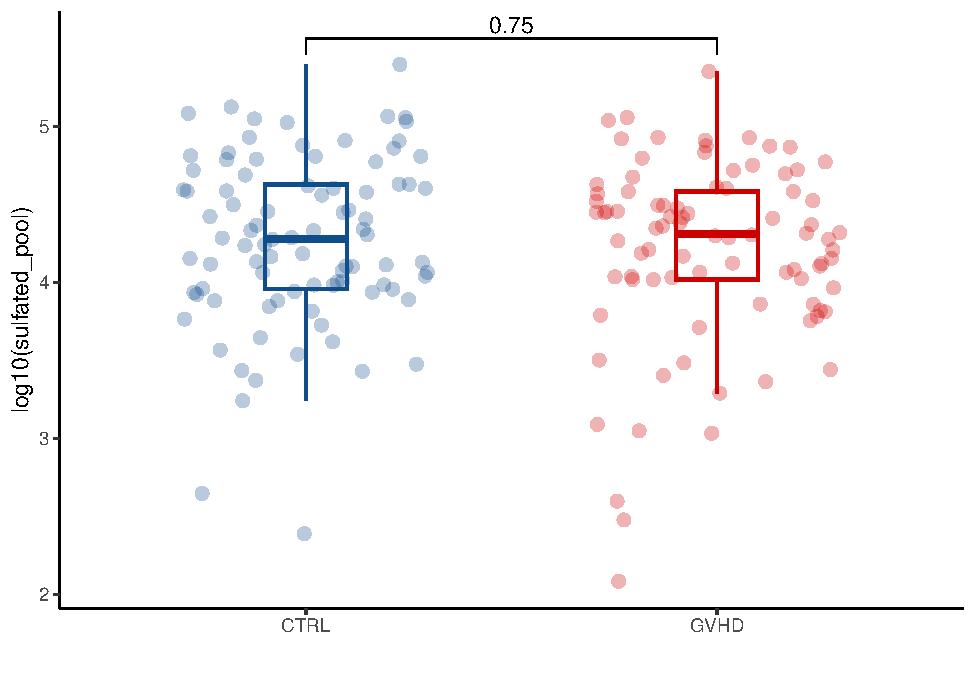
\includegraphics{_main_files/figure-latex/unnamed-chunk-14-1.pdf}

\hypertarget{create-pies-1}{%
\subsection{Create pies}\label{create-pies-1}}

\begin{Shaded}
\begin{Highlighting}[]
\NormalTok{dataset\_pre}\OtherTok{\textless{}{-}}\NormalTok{periengr\_pools\_final }\SpecialCharTok{\%\textgreater{}\%} 
  \FunctionTok{gather}\NormalTok{(}\StringTok{"BA\_pool"}\NormalTok{, }\StringTok{"value"}\NormalTok{, }\FunctionTok{names}\NormalTok{(.)[}\DecValTok{2}\NormalTok{]}\SpecialCharTok{:}\FunctionTok{names}\NormalTok{(.)[}\FunctionTok{ncol}\NormalTok{(.)]) }\SpecialCharTok{\%\textgreater{}\%} 
  \FunctionTok{left\_join}\NormalTok{(cohort\_BAS }\SpecialCharTok{\%\textgreater{}\%} \FunctionTok{select}\NormalTok{(sampleid, GI\_GVHD, ursodiol)) }\SpecialCharTok{\%\textgreater{}\%} 
  \FunctionTok{filter}\NormalTok{(ursodiol}\SpecialCharTok{==}\StringTok{"Y"}\NormalTok{) }\SpecialCharTok{\%\textgreater{}\%} 
  \FunctionTok{group\_by}\NormalTok{(GI\_GVHD, BA\_pool) }\SpecialCharTok{\%\textgreater{}\%} 
  \FunctionTok{summarise}\NormalTok{(}\AttributeTok{ave\_pool=}\FunctionTok{ave}\NormalTok{(value)) }\SpecialCharTok{\%\textgreater{}\%} \FunctionTok{slice}\NormalTok{(}\DecValTok{1}\NormalTok{)}

\NormalTok{dataset\_pre2}\OtherTok{\textless{}{-}}\NormalTok{dataset\_pre }\SpecialCharTok{\%\textgreater{}\%} 
  \FunctionTok{filter}\NormalTok{(BA\_pool}\SpecialCharTok{==}\StringTok{"primary\_pool"}\SpecialCharTok{|}\NormalTok{BA\_pool}\SpecialCharTok{==}\StringTok{"secondary\_nonUDCA"}\NormalTok{) }\SpecialCharTok{\%\textgreater{}\%} \CommentTok{\#to evaluate nonUDCA secondary and primary}
  \CommentTok{\#filter(BA\_pool=="primary\_pool"|BA\_pool=="secondary\_pool") \%\textgreater{}\% \#to evaluate total secondary}
  \CommentTok{\#filter(BA\_pool=="glycine\_pool"|BA\_pool=="taurine\_pool"|BA\_pool=="sulfated\_pool"|BA\_pool=="unconjugated\_pool") \%\textgreater{}\% }
  \FunctionTok{rename}\NormalTok{(}\AttributeTok{group=}\NormalTok{BA\_pool) }\SpecialCharTok{\%\textgreater{}\%} 
  \FunctionTok{rename}\NormalTok{(}\AttributeTok{value=}\NormalTok{ave\_pool) }\SpecialCharTok{\%\textgreater{}\%} 
  \FunctionTok{ungroup}\NormalTok{() }\SpecialCharTok{\%\textgreater{}\%} 
  \FunctionTok{group\_by}\NormalTok{(GI\_GVHD) }\SpecialCharTok{\%\textgreater{}\%} 
  \FunctionTok{mutate}\NormalTok{(}\AttributeTok{sum\_value=}\FunctionTok{sum}\NormalTok{(value)) }\SpecialCharTok{\%\textgreater{}\%} 
  \FunctionTok{mutate}\NormalTok{(}\AttributeTok{perc=}\NormalTok{value}\SpecialCharTok{/}\NormalTok{sum\_value) }\SpecialCharTok{\%\textgreater{}\%} 
  \FunctionTok{mutate}\NormalTok{(}\AttributeTok{labels =}\NormalTok{ scales}\SpecialCharTok{::}\FunctionTok{percent}\NormalTok{(perc)) }\SpecialCharTok{\%\textgreater{}\%} 
  \FunctionTok{ungroup}\NormalTok{()}

\CommentTok{\#only run to evaluate glycine/taurine conjugation }
\CommentTok{\#define order of piechart for glycine/taurin conjugation}
\CommentTok{\#dataset\_pre2$group \textless{}{-} factor(dataset\_pre2$group, levels = c("glycine\_pool", "taurine\_pool","unconjugated\_pool","sulfated\_pool"))}

\NormalTok{cp}\OtherTok{\textless{}{-}}\FunctionTok{coord\_polar}\NormalTok{(}\AttributeTok{theta=}\StringTok{"y"}\NormalTok{)}
\NormalTok{cp}\SpecialCharTok{$}\NormalTok{is\_free}\OtherTok{\textless{}{-}}\ControlFlowTok{function}\NormalTok{()}\ConstantTok{TRUE}

\FunctionTok{ggplot}\NormalTok{(dataset\_pre2, }\FunctionTok{aes}\NormalTok{(}\AttributeTok{x=}\StringTok{""}\NormalTok{, }\AttributeTok{y=}\NormalTok{perc, }\AttributeTok{fill=}\NormalTok{group))}\SpecialCharTok{+}
  \FunctionTok{geom\_bar}\NormalTok{(}\AttributeTok{stat=}\StringTok{"identity"}\NormalTok{, }\AttributeTok{width=}\DecValTok{1}\NormalTok{)}\SpecialCharTok{+}\NormalTok{cp}\SpecialCharTok{+}
  \FunctionTok{facet\_wrap}\NormalTok{(.}\SpecialCharTok{\textasciitilde{}}\NormalTok{GI\_GVHD, }\AttributeTok{scales=}\StringTok{"free"}\NormalTok{)}\SpecialCharTok{+}
  \FunctionTok{geom\_text}\NormalTok{(}\FunctionTok{aes}\NormalTok{(}\AttributeTok{label =}\NormalTok{ labels),}
            \AttributeTok{position =} \FunctionTok{position\_stack}\NormalTok{(}\AttributeTok{vjust =} \FloatTok{0.5}\NormalTok{)) }\SpecialCharTok{+}
  \FunctionTok{theme\_void}\NormalTok{()}\SpecialCharTok{+}
  \FunctionTok{theme}\NormalTok{(}\AttributeTok{axis.ticks=}\FunctionTok{element\_blank}\NormalTok{(),}
        \AttributeTok{axis.title=}\FunctionTok{element\_blank}\NormalTok{(),}
        \AttributeTok{axis.text.y=}\FunctionTok{element\_blank}\NormalTok{())}\SpecialCharTok{+}
  \CommentTok{\#scale\_fill\_manual(values=c("green4","chartreuse3","dodgerblue2","purple2"))}
  \FunctionTok{scale\_fill\_manual}\NormalTok{(}\AttributeTok{values=}\FunctionTok{c}\NormalTok{(}\StringTok{"\#E7861B"}\NormalTok{,}\StringTok{"darkgoldenrod1"}\NormalTok{)) }\CommentTok{\#for primary/secondary}
\end{Highlighting}
\end{Shaded}

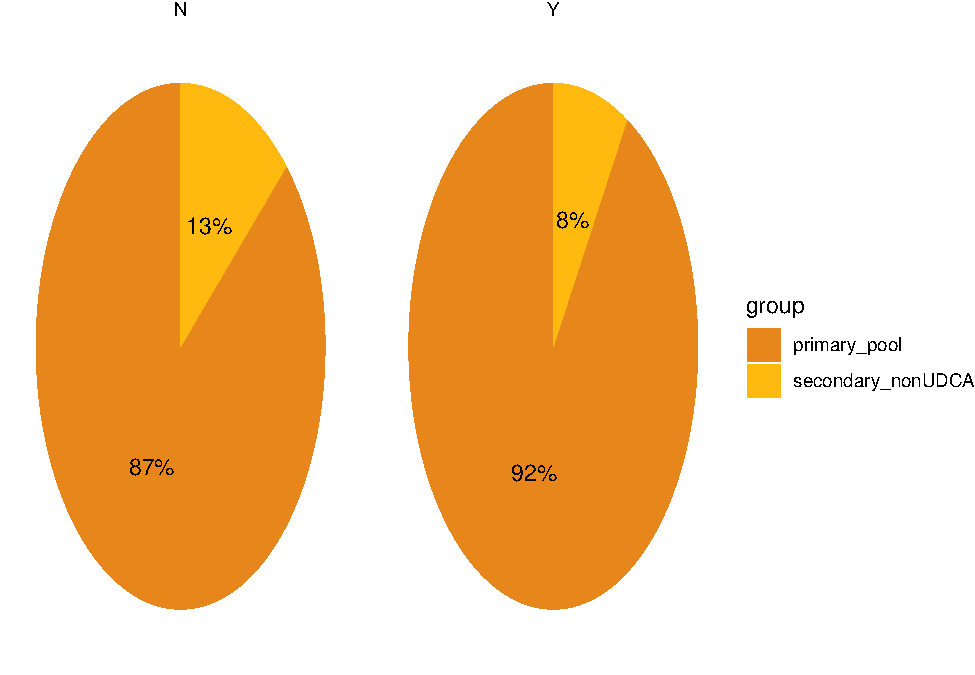
\includegraphics{_main_files/figure-latex/unnamed-chunk-15-1.pdf}

\hypertarget{evaluate-t-cell-modulatory-bas-in-patients-with-gvhd-vs-controls-figure-4}{%
\chapter{Evaluate T cell modulatory BAs in patients with GVHD vs controls (figure 4)}\label{evaluate-t-cell-modulatory-bas-in-patients-with-gvhd-vs-controls-figure-4}}

\hypertarget{oxolca}{%
\section{3oxoLCA}\label{oxolca}}

\begin{Shaded}
\begin{Highlighting}[]
\NormalTok{filtered\_combined\_table }\SpecialCharTok{\%\textgreater{}\%} 
  \FunctionTok{left\_join}\NormalTok{(cohort\_BAS) }\SpecialCharTok{\%\textgreater{}\%} 
  \FunctionTok{filter}\NormalTok{(later}\SpecialCharTok{==}\StringTok{"Y"}\NormalTok{) }\SpecialCharTok{\%\textgreater{}\%} 
  \FunctionTok{filter}\NormalTok{(ursodiol}\SpecialCharTok{==}\StringTok{"Y"}\NormalTok{) }\SpecialCharTok{\%\textgreater{}\%} 
  \FunctionTok{ggplot}\NormalTok{(}\FunctionTok{aes}\NormalTok{(}\AttributeTok{y=}\FunctionTok{log10}\NormalTok{(dehydrolithocholic\_acid}\SpecialCharTok{+}\DecValTok{25000}\NormalTok{), }\AttributeTok{x=}\NormalTok{GI\_GVHD, }\AttributeTok{color=}\NormalTok{GI\_GVHD))}\SpecialCharTok{+}
  \FunctionTok{geom\_boxplot}\NormalTok{(}\AttributeTok{width=}\FloatTok{0.2}\NormalTok{, }\AttributeTok{lwd=}\FloatTok{0.8}\NormalTok{, }\AttributeTok{outlier.shape =} \ConstantTok{NA}\NormalTok{) }\SpecialCharTok{+}
  \FunctionTok{geom\_jitter}\NormalTok{(}\AttributeTok{width=}\FloatTok{0.3}\NormalTok{, }\AttributeTok{alpha=}\FloatTok{0.3}\NormalTok{, }\AttributeTok{size=}\FloatTok{2.5}\NormalTok{)}\SpecialCharTok{+}
  \FunctionTok{ylab}\NormalTok{(}\StringTok{"log10(3oxoLCA)"}\NormalTok{)}\SpecialCharTok{+}
  \FunctionTok{xlab}\NormalTok{(}\StringTok{""}\NormalTok{)}\SpecialCharTok{+}
  \FunctionTok{theme\_classic}\NormalTok{()}\SpecialCharTok{+}
  \FunctionTok{stat\_compare\_means}\NormalTok{(}\AttributeTok{comparisons=}\FunctionTok{list}\NormalTok{(}\FunctionTok{c}\NormalTok{(}\StringTok{"Y"}\NormalTok{, }\StringTok{"N"}\NormalTok{)),}
                     \AttributeTok{method=}\StringTok{"wilcox.test"}\NormalTok{,}
                     \AttributeTok{correct=}\ConstantTok{FALSE}\NormalTok{)}\SpecialCharTok{+}
  \FunctionTok{scale\_color\_manual}\NormalTok{(}\AttributeTok{values=}\FunctionTok{c}\NormalTok{(}\StringTok{"dodgerblue4"}\NormalTok{, }\StringTok{"red3"}\NormalTok{))}\SpecialCharTok{+}
  \FunctionTok{theme}\NormalTok{(}\AttributeTok{legend.position=}\StringTok{"none"}\NormalTok{)}
\end{Highlighting}
\end{Shaded}

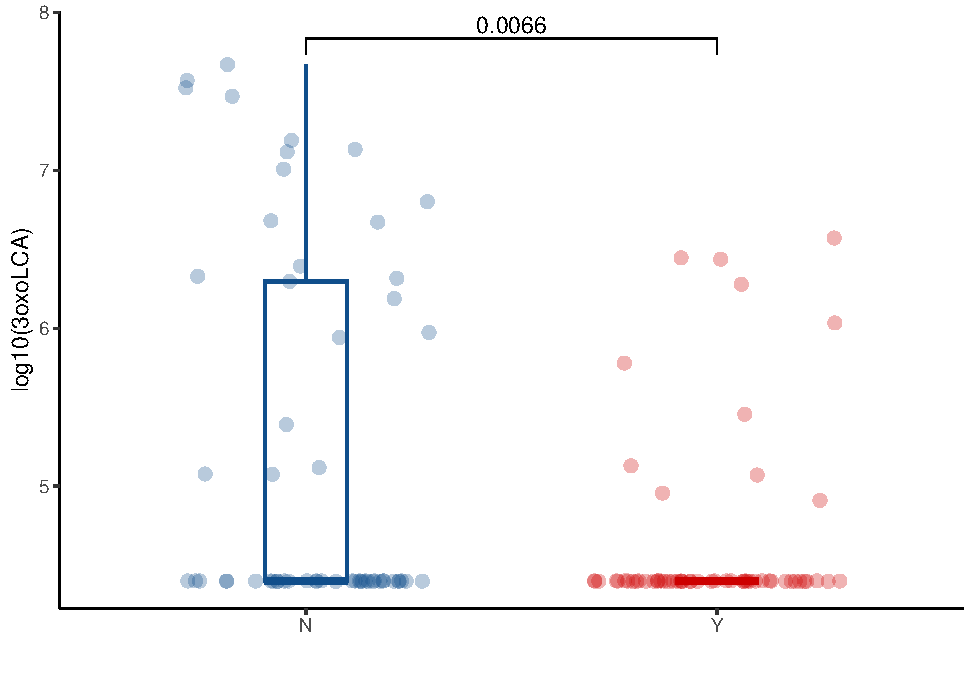
\includegraphics{_main_files/figure-latex/unnamed-chunk-16-1.pdf}

\hypertarget{isolca}{%
\section{isoLCA}\label{isolca}}

\begin{Shaded}
\begin{Highlighting}[]
\NormalTok{filtered\_combined\_table }\SpecialCharTok{\%\textgreater{}\%} 
  \FunctionTok{left\_join}\NormalTok{(cohort\_BAS) }\SpecialCharTok{\%\textgreater{}\%} 
  \FunctionTok{filter}\NormalTok{(later}\SpecialCharTok{==}\StringTok{"Y"}\NormalTok{) }\SpecialCharTok{\%\textgreater{}\%} 
  \FunctionTok{filter}\NormalTok{(ursodiol}\SpecialCharTok{==}\StringTok{"Y"}\NormalTok{) }\SpecialCharTok{\%\textgreater{}\%} 
  \FunctionTok{ggplot}\NormalTok{(}\FunctionTok{aes}\NormalTok{(}\AttributeTok{y=}\FunctionTok{log10}\NormalTok{(isolithocholic\_acid}\SpecialCharTok{+}\DecValTok{25000}\NormalTok{), }\AttributeTok{x=}\NormalTok{GI\_GVHD, }\AttributeTok{color=}\NormalTok{GI\_GVHD))}\SpecialCharTok{+}
  \FunctionTok{geom\_boxplot}\NormalTok{(}\AttributeTok{width=}\FloatTok{0.2}\NormalTok{, }\AttributeTok{lwd=}\FloatTok{0.8}\NormalTok{, }\AttributeTok{outlier.shape =} \ConstantTok{NA}\NormalTok{) }\SpecialCharTok{+}
  \FunctionTok{geom\_jitter}\NormalTok{(}\AttributeTok{width=}\FloatTok{0.3}\NormalTok{, }\AttributeTok{alpha=}\FloatTok{0.3}\NormalTok{, }\AttributeTok{size=}\FloatTok{2.5}\NormalTok{)}\SpecialCharTok{+}
  \FunctionTok{ylab}\NormalTok{(}\StringTok{"log10(isoLCA)"}\NormalTok{)}\SpecialCharTok{+}
  \FunctionTok{xlab}\NormalTok{(}\StringTok{""}\NormalTok{)}\SpecialCharTok{+}
  \FunctionTok{theme\_classic}\NormalTok{()}\SpecialCharTok{+}
  \FunctionTok{stat\_compare\_means}\NormalTok{(}\AttributeTok{comparisons=}\FunctionTok{list}\NormalTok{(}\FunctionTok{c}\NormalTok{(}\StringTok{"Y"}\NormalTok{, }\StringTok{"N"}\NormalTok{)),}
                     \AttributeTok{method=}\StringTok{"wilcox.test"}\NormalTok{,}
                     \AttributeTok{correct=}\ConstantTok{FALSE}\NormalTok{)}\SpecialCharTok{+}
  \FunctionTok{scale\_color\_manual}\NormalTok{(}\AttributeTok{values=}\FunctionTok{c}\NormalTok{(}\StringTok{"dodgerblue4"}\NormalTok{, }\StringTok{"red3"}\NormalTok{))}\SpecialCharTok{+}
  \FunctionTok{theme}\NormalTok{(}\AttributeTok{legend.position=}\StringTok{"none"}\NormalTok{)}
\end{Highlighting}
\end{Shaded}

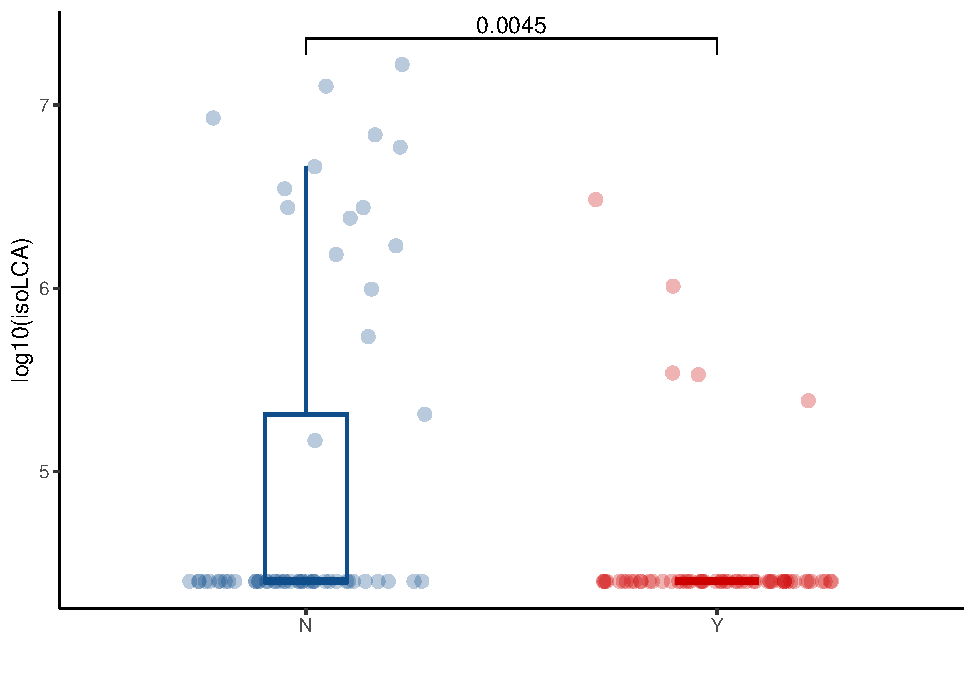
\includegraphics{_main_files/figure-latex/unnamed-chunk-17-1.pdf}

\hypertarget{isodca}{%
\section{isoDCA}\label{isodca}}

\begin{Shaded}
\begin{Highlighting}[]
\NormalTok{filtered\_combined\_table }\SpecialCharTok{\%\textgreater{}\%} 
  \FunctionTok{left\_join}\NormalTok{(cohort\_BAS) }\SpecialCharTok{\%\textgreater{}\%} 
  \FunctionTok{filter}\NormalTok{(later}\SpecialCharTok{==}\StringTok{"Y"}\NormalTok{) }\SpecialCharTok{\%\textgreater{}\%} 
  \FunctionTok{filter}\NormalTok{(ursodiol}\SpecialCharTok{==}\StringTok{"Y"}\NormalTok{) }\SpecialCharTok{\%\textgreater{}\%} 
  \FunctionTok{ggplot}\NormalTok{(}\FunctionTok{aes}\NormalTok{(}\AttributeTok{y=}\FunctionTok{log10}\NormalTok{(isodeoxycholic\_acid}\SpecialCharTok{+}\DecValTok{25000}\NormalTok{), }\AttributeTok{x=}\NormalTok{GI\_GVHD, }\AttributeTok{color=}\NormalTok{GI\_GVHD))}\SpecialCharTok{+}
  \FunctionTok{geom\_boxplot}\NormalTok{(}\AttributeTok{width=}\FloatTok{0.2}\NormalTok{, }\AttributeTok{lwd=}\FloatTok{0.8}\NormalTok{, }\AttributeTok{outlier.shape =} \ConstantTok{NA}\NormalTok{) }\SpecialCharTok{+}
  \FunctionTok{geom\_jitter}\NormalTok{(}\AttributeTok{width=}\FloatTok{0.3}\NormalTok{, }\AttributeTok{alpha=}\FloatTok{0.3}\NormalTok{, }\AttributeTok{size=}\FloatTok{2.5}\NormalTok{)}\SpecialCharTok{+}
  \FunctionTok{ylab}\NormalTok{(}\StringTok{"log10(isoDCA)"}\NormalTok{)}\SpecialCharTok{+}
  \FunctionTok{xlab}\NormalTok{(}\StringTok{""}\NormalTok{)}\SpecialCharTok{+}
  \FunctionTok{theme\_classic}\NormalTok{()}\SpecialCharTok{+}
  \FunctionTok{stat\_compare\_means}\NormalTok{(}\AttributeTok{comparisons=}\FunctionTok{list}\NormalTok{(}\FunctionTok{c}\NormalTok{(}\StringTok{"Y"}\NormalTok{, }\StringTok{"N"}\NormalTok{)),}
                     \AttributeTok{method=}\StringTok{"wilcox.test"}\NormalTok{,}
                     \AttributeTok{correct=}\ConstantTok{FALSE}\NormalTok{)}\SpecialCharTok{+}
  \FunctionTok{scale\_color\_manual}\NormalTok{(}\AttributeTok{values=}\FunctionTok{c}\NormalTok{(}\StringTok{"dodgerblue4"}\NormalTok{, }\StringTok{"red3"}\NormalTok{))}\SpecialCharTok{+}
  \FunctionTok{theme}\NormalTok{(}\AttributeTok{legend.position=}\StringTok{"none"}\NormalTok{)}
\end{Highlighting}
\end{Shaded}

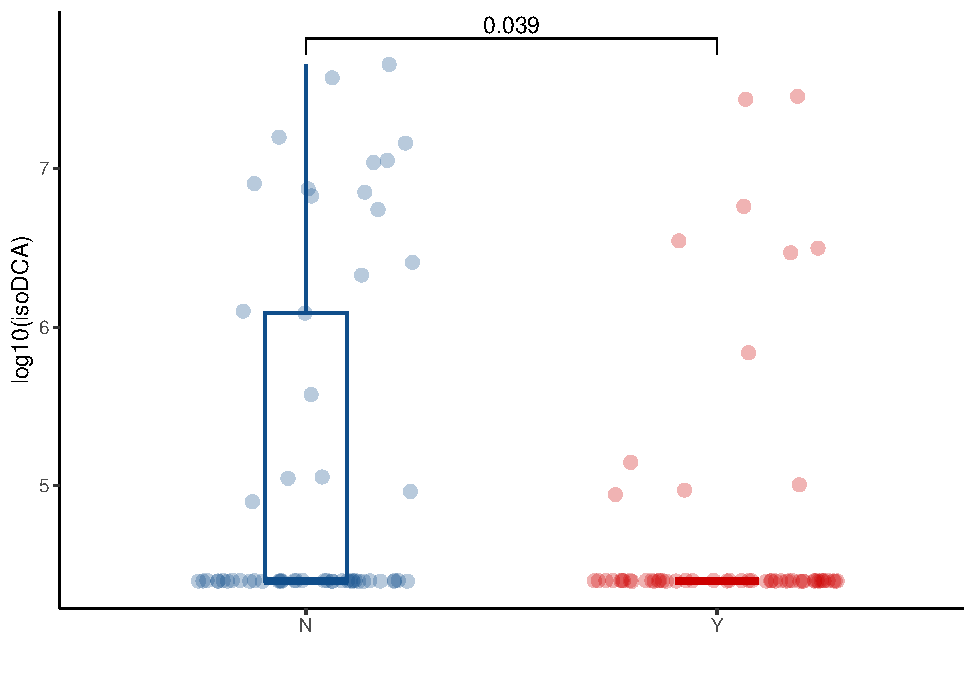
\includegraphics{_main_files/figure-latex/unnamed-chunk-18-1.pdf}

\hypertarget{omca}{%
\section{OMCA}\label{omca}}

\begin{Shaded}
\begin{Highlighting}[]
\NormalTok{conc\_all\_filtered }\SpecialCharTok{\%\textgreater{}\%} 
  \FunctionTok{left\_join}\NormalTok{(cohort\_BAS) }\SpecialCharTok{\%\textgreater{}\%} 
  \FunctionTok{filter}\NormalTok{(later}\SpecialCharTok{==}\StringTok{"Y"}\NormalTok{) }\SpecialCharTok{\%\textgreater{}\%} 
  \FunctionTok{filter}\NormalTok{(ursodiol}\SpecialCharTok{==}\StringTok{"Y"}\NormalTok{) }\SpecialCharTok{\%\textgreater{}\%} 
  \FunctionTok{ggplot}\NormalTok{(}\FunctionTok{aes}\NormalTok{(}\AttributeTok{y=}\FunctionTok{log10}\NormalTok{(omega\_muricholic\_acid}\FloatTok{+2.5}\NormalTok{), }\AttributeTok{x=}\NormalTok{GI\_GVHD, }\AttributeTok{color=}\NormalTok{GI\_GVHD))}\SpecialCharTok{+}
  \FunctionTok{geom\_boxplot}\NormalTok{(}\AttributeTok{width=}\FloatTok{0.2}\NormalTok{, }\AttributeTok{lwd=}\FloatTok{0.8}\NormalTok{, }\AttributeTok{outlier.shape =} \ConstantTok{NA}\NormalTok{) }\SpecialCharTok{+}
  \FunctionTok{geom\_jitter}\NormalTok{(}\AttributeTok{width=}\FloatTok{0.3}\NormalTok{, }\AttributeTok{alpha=}\FloatTok{0.3}\NormalTok{, }\AttributeTok{size=}\FloatTok{2.5}\NormalTok{)}\SpecialCharTok{+}
  \FunctionTok{ylab}\NormalTok{(}\StringTok{"log10(OMCA)"}\NormalTok{)}\SpecialCharTok{+}
  \FunctionTok{xlab}\NormalTok{(}\StringTok{""}\NormalTok{)}\SpecialCharTok{+}
  \FunctionTok{theme\_classic}\NormalTok{()}\SpecialCharTok{+}
  \FunctionTok{stat\_compare\_means}\NormalTok{(}\AttributeTok{comparisons=}\FunctionTok{list}\NormalTok{(}\FunctionTok{c}\NormalTok{(}\StringTok{"Y"}\NormalTok{, }\StringTok{"N"}\NormalTok{)),}
                     \AttributeTok{method=}\StringTok{"wilcox.test"}\NormalTok{,}
                     \AttributeTok{correct=}\ConstantTok{FALSE}\NormalTok{)}\SpecialCharTok{+}
  \FunctionTok{scale\_color\_manual}\NormalTok{(}\AttributeTok{values=}\FunctionTok{c}\NormalTok{(}\StringTok{"dodgerblue4"}\NormalTok{, }\StringTok{"red3"}\NormalTok{))}\SpecialCharTok{+}
  \FunctionTok{theme}\NormalTok{(}\AttributeTok{legend.position=}\StringTok{"none"}\NormalTok{)}
\end{Highlighting}
\end{Shaded}

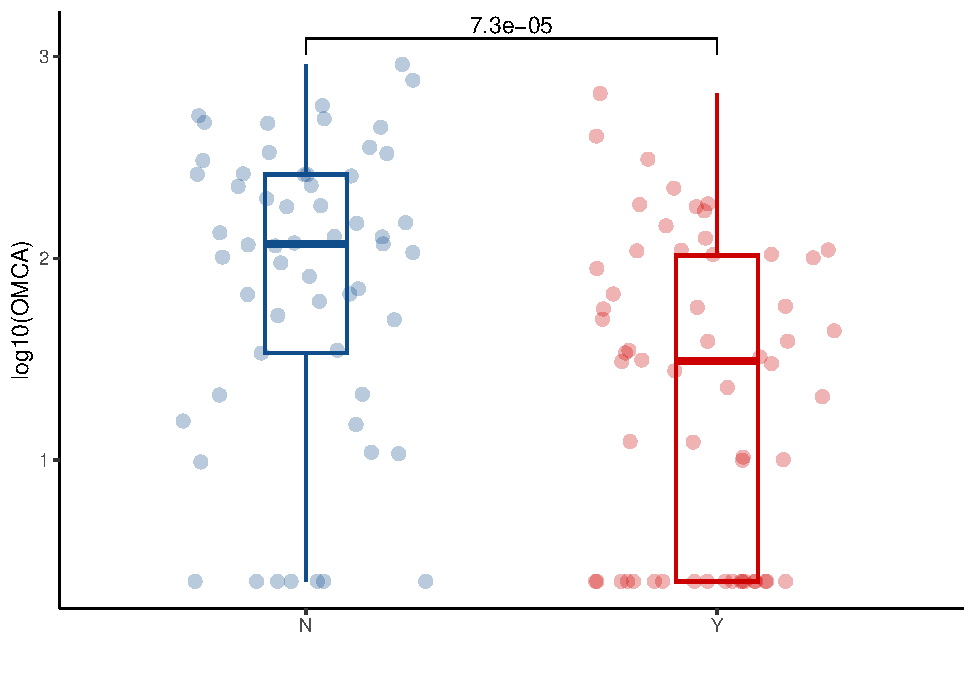
\includegraphics{_main_files/figure-latex/unnamed-chunk-19-1.pdf}

\hypertarget{shotgun-metagenomic-sequencing-evaluate-genes-of-interest-figure-5-supplement-figure-10}{%
\chapter{Shotgun metagenomic sequencing: Evaluate genes of interest (figure 5, supplement figure 10)}\label{shotgun-metagenomic-sequencing-evaluate-genes-of-interest-figure-5-supplement-figure-10}}

\hypertarget{bsh}{%
\section{BSH}\label{bsh}}

\hypertarget{evaluate-bsh-abundance-at-peri-gvhd-onset}{%
\subsection{Evaluate BSH abundance at peri-GVHD onset}\label{evaluate-bsh-abundance-at-peri-gvhd-onset}}

\begin{Shaded}
\begin{Highlighting}[]
\NormalTok{BSH\_metalphlan }\SpecialCharTok{\%\textgreater{}\%} 
  \FunctionTok{left\_join}\NormalTok{(cohort\_BAS) }\SpecialCharTok{\%\textgreater{}\%} 
  \FunctionTok{filter}\NormalTok{(later}\SpecialCharTok{==}\StringTok{"Y"}\NormalTok{) }\SpecialCharTok{\%\textgreater{}\%} 
  \FunctionTok{ggplot}\NormalTok{(}\FunctionTok{aes}\NormalTok{(}\AttributeTok{x=}\NormalTok{GI\_GVHD, }\AttributeTok{y=}\FunctionTok{log10}\NormalTok{(cpm}\FloatTok{+0.55}\NormalTok{), }\AttributeTok{color=}\NormalTok{GI\_GVHD))}\SpecialCharTok{+}
  \FunctionTok{geom\_boxplot}\NormalTok{(}\AttributeTok{width=}\FloatTok{0.2}\NormalTok{, }\AttributeTok{lwd=}\FloatTok{0.8}\NormalTok{, }\AttributeTok{outlier.shape =} \ConstantTok{NA}\NormalTok{) }\SpecialCharTok{+}
  \FunctionTok{geom\_jitter}\NormalTok{(}\AttributeTok{width=}\FloatTok{0.3}\NormalTok{, }\AttributeTok{alpha=}\FloatTok{0.3}\NormalTok{, }\AttributeTok{size=}\FloatTok{2.5}\NormalTok{)}\SpecialCharTok{+}
  \FunctionTok{ylab}\NormalTok{(}\StringTok{"log10(BSH)"}\NormalTok{)}\SpecialCharTok{+}
  \FunctionTok{xlab}\NormalTok{(}\StringTok{""}\NormalTok{)}\SpecialCharTok{+}
  \FunctionTok{theme\_classic}\NormalTok{()}\SpecialCharTok{+}
  \FunctionTok{stat\_compare\_means}\NormalTok{(}\AttributeTok{comparisons=}\FunctionTok{list}\NormalTok{(}\FunctionTok{c}\NormalTok{(}\StringTok{"Y"}\NormalTok{, }\StringTok{"N"}\NormalTok{)),}
                     \AttributeTok{method=}\StringTok{"wilcox.test"}\NormalTok{,}
                     \AttributeTok{correct=}\ConstantTok{FALSE}\NormalTok{)}\SpecialCharTok{+}
  \FunctionTok{scale\_color\_manual}\NormalTok{(}\AttributeTok{values=}\FunctionTok{c}\NormalTok{(}\StringTok{"dodgerblue4"}\NormalTok{, }\StringTok{"red3"}\NormalTok{))}\SpecialCharTok{+}
  \FunctionTok{theme}\NormalTok{(}\AttributeTok{legend.position=}\StringTok{"none"}\NormalTok{)}
\end{Highlighting}
\end{Shaded}

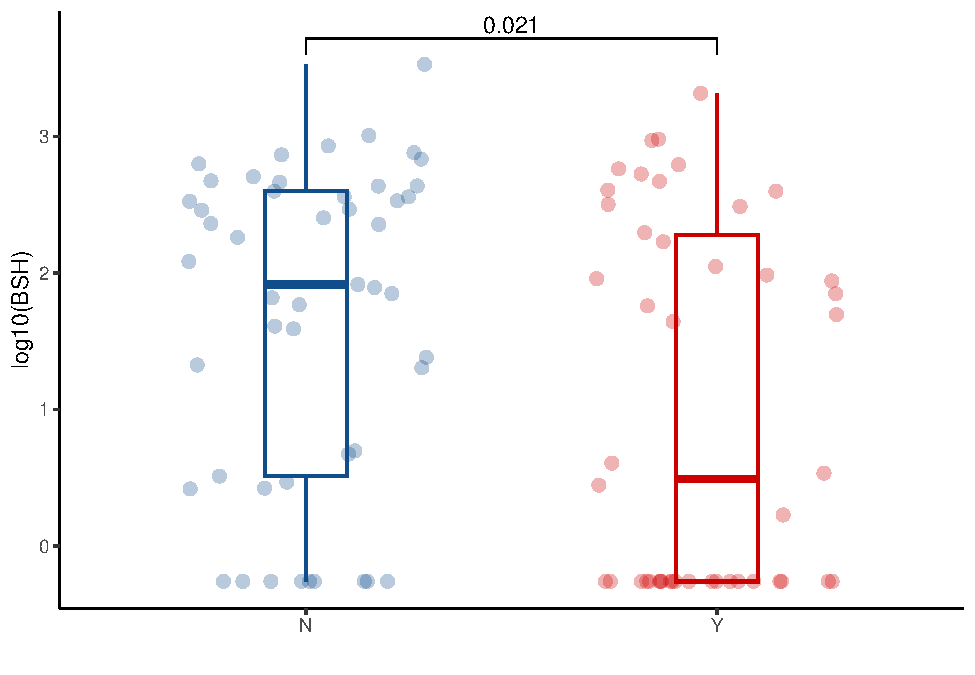
\includegraphics{_main_files/figure-latex/unnamed-chunk-20-1.pdf}

\hypertarget{evaluate-bsh-abundance-at-peri-engraftment-time-point}{%
\subsection{Evaluate BSH abundance at peri-engraftment time point}\label{evaluate-bsh-abundance-at-peri-engraftment-time-point}}

\begin{Shaded}
\begin{Highlighting}[]
\NormalTok{BSH\_metalphlan }\SpecialCharTok{\%\textgreater{}\%} 
  \FunctionTok{left\_join}\NormalTok{(cohort\_BAS) }\SpecialCharTok{\%\textgreater{}\%} 
  \FunctionTok{filter}\NormalTok{(periengr}\SpecialCharTok{==}\StringTok{"Y"}\NormalTok{) }\SpecialCharTok{\%\textgreater{}\%} 
  \FunctionTok{ggplot}\NormalTok{(}\FunctionTok{aes}\NormalTok{(}\AttributeTok{x=}\NormalTok{GI\_GVHD, }\AttributeTok{y=}\FunctionTok{log10}\NormalTok{(cpm}\FloatTok{+0.05}\NormalTok{), }\AttributeTok{color=}\NormalTok{GI\_GVHD))}\SpecialCharTok{+}
  \FunctionTok{geom\_boxplot}\NormalTok{(}\AttributeTok{width=}\FloatTok{0.2}\NormalTok{, }\AttributeTok{lwd=}\FloatTok{0.8}\NormalTok{, }\AttributeTok{outlier.shape =} \ConstantTok{NA}\NormalTok{) }\SpecialCharTok{+}
  \FunctionTok{geom\_jitter}\NormalTok{(}\AttributeTok{width=}\FloatTok{0.3}\NormalTok{, }\AttributeTok{alpha=}\FloatTok{0.3}\NormalTok{, }\AttributeTok{size=}\FloatTok{2.5}\NormalTok{)}\SpecialCharTok{+}
  \FunctionTok{ylab}\NormalTok{(}\StringTok{"log10(BSH)"}\NormalTok{)}\SpecialCharTok{+}
  \FunctionTok{xlab}\NormalTok{(}\StringTok{""}\NormalTok{)}\SpecialCharTok{+}
  \FunctionTok{theme\_classic}\NormalTok{()}\SpecialCharTok{+}
  \FunctionTok{stat\_compare\_means}\NormalTok{(}\AttributeTok{comparisons=}\FunctionTok{list}\NormalTok{(}\FunctionTok{c}\NormalTok{(}\StringTok{"Y"}\NormalTok{, }\StringTok{"N"}\NormalTok{)),}
                     \AttributeTok{method=}\StringTok{"wilcox.test"}\NormalTok{,}
                     \AttributeTok{correct=}\ConstantTok{FALSE}\NormalTok{)}\SpecialCharTok{+}
  \FunctionTok{scale\_color\_manual}\NormalTok{(}\AttributeTok{values=}\FunctionTok{c}\NormalTok{(}\StringTok{"dodgerblue4"}\NormalTok{, }\StringTok{"red3"}\NormalTok{))}\SpecialCharTok{+}
  \FunctionTok{theme}\NormalTok{(}\AttributeTok{legend.position=}\StringTok{"none"}\NormalTok{)}
\end{Highlighting}
\end{Shaded}

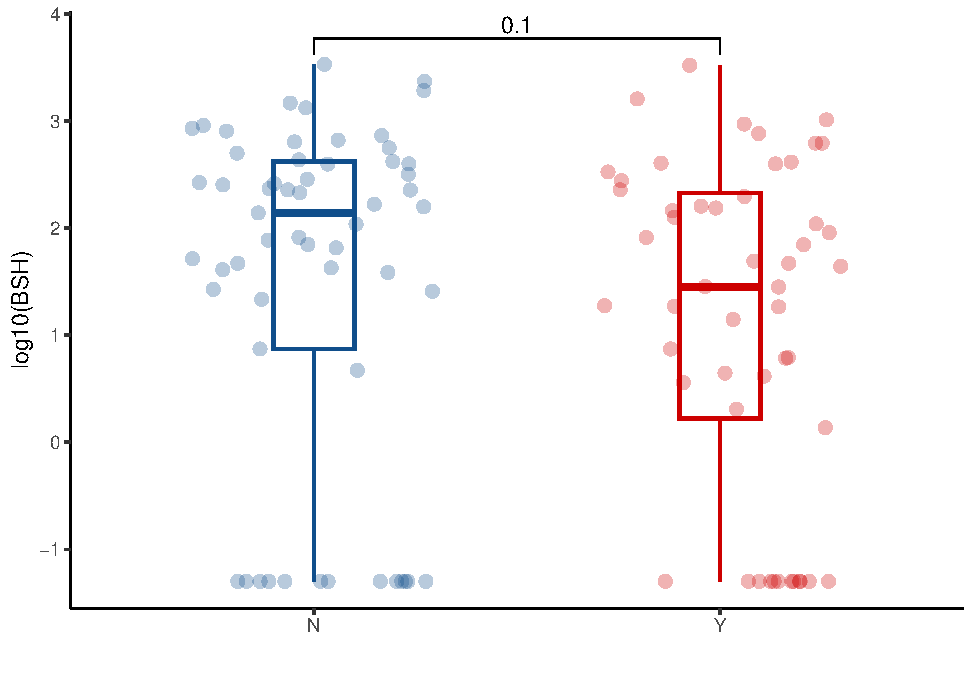
\includegraphics{_main_files/figure-latex/unnamed-chunk-21-1.pdf}

\hypertarget{bai-operon-gene}{%
\section{Bai operon gene}\label{bai-operon-gene}}

\hypertarget{evaluate-correlation-of-bai-operon-gene-sum-and-nonudca-secondary-bas}{%
\subsection{Evaluate correlation of bai operon gene sum and nonUDCA secondary BAs}\label{evaluate-correlation-of-bai-operon-gene-sum-and-nonudca-secondary-bas}}

\begin{Shaded}
\begin{Highlighting}[]
\NormalTok{bai\_genes\_clean }\SpecialCharTok{\%\textgreater{}\%} 
  \FunctionTok{distinct}\NormalTok{(sampleid, bai\_operon\_sum ) }\SpecialCharTok{\%\textgreater{}\%} 
  \FunctionTok{inner\_join}\NormalTok{(both\_conc\_pools\_final) }\SpecialCharTok{\%\textgreater{}\%} 
  \FunctionTok{ggplot}\NormalTok{(}\FunctionTok{aes}\NormalTok{(}\AttributeTok{x=}\FunctionTok{log}\NormalTok{(secondary\_nonUDCA), }\AttributeTok{y=}\FunctionTok{log}\NormalTok{(bai\_operon\_sum}\FloatTok{+0.05}\NormalTok{)))}\SpecialCharTok{+}
  \FunctionTok{geom\_point}\NormalTok{(}\AttributeTok{alpha=}\FloatTok{0.6}\NormalTok{)}\SpecialCharTok{+}
  \FunctionTok{stat\_cor}\NormalTok{(}\AttributeTok{method=}\StringTok{"pearson"}\NormalTok{)}\SpecialCharTok{+}
  \FunctionTok{geom\_smooth}\NormalTok{(}\AttributeTok{method=}\StringTok{"lm"}\NormalTok{)}\SpecialCharTok{+}
  \FunctionTok{theme\_classic}\NormalTok{()}\SpecialCharTok{+}
  \FunctionTok{ylab}\NormalTok{(}\StringTok{"bai operon log10(cpm)"}\NormalTok{)}\SpecialCharTok{+}
  \FunctionTok{xlab}\NormalTok{(}\StringTok{"SBAs* log10(pmol/mg)"}\NormalTok{)}
\end{Highlighting}
\end{Shaded}

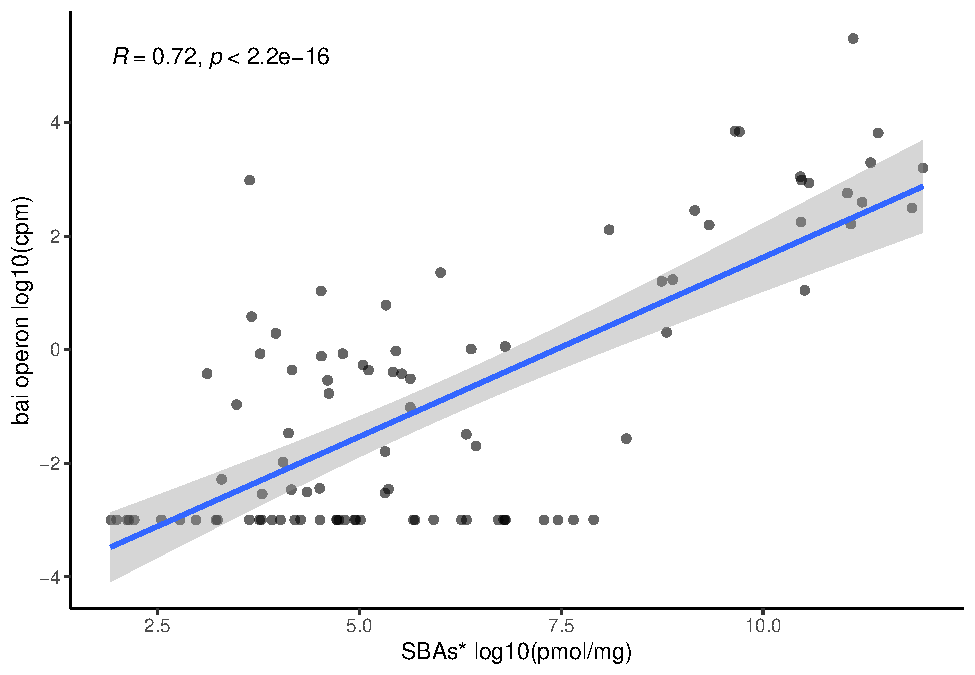
\includegraphics{_main_files/figure-latex/unnamed-chunk-22-1.pdf}

\hypertarget{bai-operon-gene-sum-in-peri-gvhd-onset}{%
\subsection{Bai operon gene sum in peri-GVHD onset}\label{bai-operon-gene-sum-in-peri-gvhd-onset}}

\begin{Shaded}
\begin{Highlighting}[]
\NormalTok{bai\_genes\_clean }\SpecialCharTok{\%\textgreater{}\%} 
  \FunctionTok{distinct}\NormalTok{(sampleid, bai\_operon\_sum ) }\SpecialCharTok{\%\textgreater{}\%} 
  \FunctionTok{inner\_join}\NormalTok{(cohort\_BAS }\SpecialCharTok{\%\textgreater{}\%} \FunctionTok{select}\NormalTok{(sampleid, GI\_GVHD, later) }\SpecialCharTok{\%\textgreater{}\%} \FunctionTok{filter}\NormalTok{(later}\SpecialCharTok{==}\StringTok{"Y"}\NormalTok{)) }\SpecialCharTok{\%\textgreater{}\%} 
  \FunctionTok{ggplot}\NormalTok{(}\FunctionTok{aes}\NormalTok{(}\AttributeTok{x=}\NormalTok{GI\_GVHD, }\AttributeTok{y=}\FunctionTok{log}\NormalTok{(bai\_operon\_sum}\FloatTok{+0.01}\NormalTok{), }\AttributeTok{color=}\NormalTok{GI\_GVHD))}\SpecialCharTok{+}
  \FunctionTok{geom\_boxplot}\NormalTok{(}\AttributeTok{width=}\FloatTok{0.2}\NormalTok{, }\AttributeTok{lwd=}\FloatTok{0.8}\NormalTok{, }\AttributeTok{outlier.shape =} \ConstantTok{NA}\NormalTok{) }\SpecialCharTok{+}
  \FunctionTok{geom\_jitter}\NormalTok{(}\AttributeTok{width=}\FloatTok{0.3}\NormalTok{, }\AttributeTok{alpha=}\FloatTok{0.3}\NormalTok{, }\AttributeTok{size=}\FloatTok{2.5}\NormalTok{) }\SpecialCharTok{+}
  \FunctionTok{ylab}\NormalTok{(}\StringTok{"log10(bai\_operon\_sum)"}\NormalTok{) }\SpecialCharTok{+}
  \FunctionTok{xlab}\NormalTok{(}\StringTok{""}\NormalTok{) }\SpecialCharTok{+}
  \FunctionTok{theme\_classic}\NormalTok{() }\SpecialCharTok{+}
  \FunctionTok{stat\_compare\_means}\NormalTok{(}\AttributeTok{comparisons=}\FunctionTok{list}\NormalTok{(}\FunctionTok{c}\NormalTok{(}\StringTok{"Y"}\NormalTok{, }\StringTok{"N"}\NormalTok{)),}
                     \AttributeTok{method=}\StringTok{"wilcox.test"}\NormalTok{,}
                     \AttributeTok{correct=}\ConstantTok{FALSE}\NormalTok{)}\SpecialCharTok{+}
  \FunctionTok{scale\_color\_manual}\NormalTok{(}\AttributeTok{values=}\FunctionTok{c}\NormalTok{(}\StringTok{"dodgerblue4"}\NormalTok{, }\StringTok{"red3"}\NormalTok{)) }\SpecialCharTok{+}
  \FunctionTok{theme}\NormalTok{(}\AttributeTok{legend.position=}\StringTok{"none"}\NormalTok{)}
\end{Highlighting}
\end{Shaded}

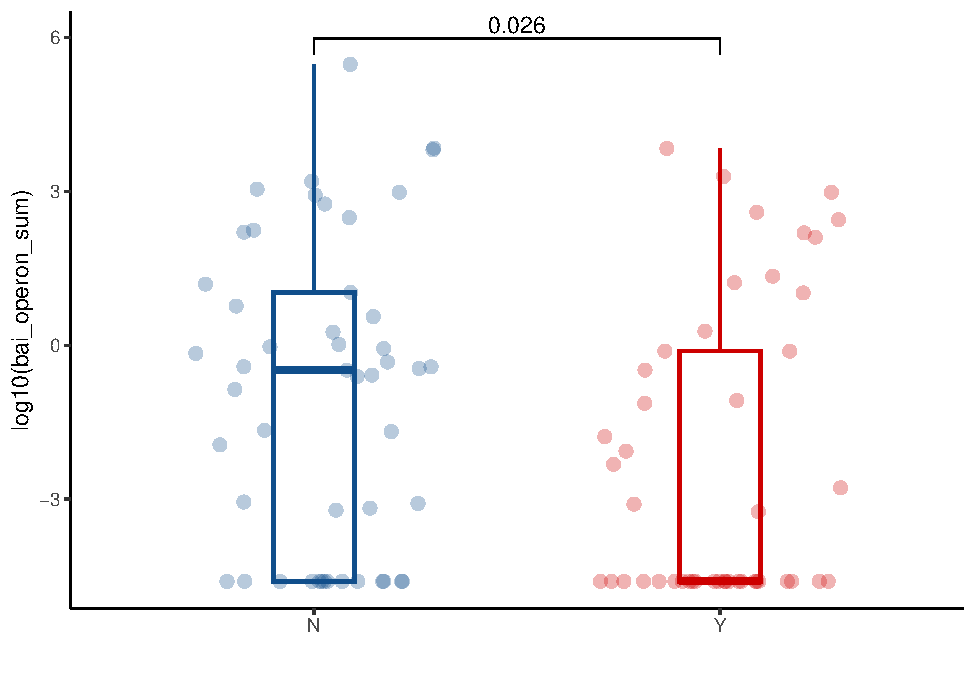
\includegraphics{_main_files/figure-latex/unnamed-chunk-23-1.pdf}

\hypertarget{bai-operon-individual-gene-abundance}{%
\subsection{Bai operon individual gene abundance}\label{bai-operon-individual-gene-abundance}}

\begin{Shaded}
\begin{Highlighting}[]
\NormalTok{bai\_genes\_clean }\SpecialCharTok{\%\textgreater{}\%} 
  \FunctionTok{inner\_join}\NormalTok{(cohort\_BAS }\SpecialCharTok{\%\textgreater{}\%} \FunctionTok{select}\NormalTok{(sampleid, GI\_GVHD, later) }\SpecialCharTok{\%\textgreater{}\%} \FunctionTok{filter}\NormalTok{(later}\SpecialCharTok{==}\StringTok{"Y"}\NormalTok{)) }\SpecialCharTok{\%\textgreater{}\%} 
  \FunctionTok{ggplot}\NormalTok{(}\FunctionTok{aes}\NormalTok{(}\AttributeTok{x=}\NormalTok{GI\_GVHD, }\AttributeTok{y=}\FunctionTok{log}\NormalTok{(cpm}\FloatTok{+0.01}\NormalTok{), }\AttributeTok{color=}\NormalTok{GI\_GVHD))}\SpecialCharTok{+}
  \FunctionTok{geom\_boxplot}\NormalTok{(}\AttributeTok{width=}\FloatTok{0.2}\NormalTok{, }\AttributeTok{lwd=}\FloatTok{0.8}\NormalTok{, }\AttributeTok{outlier.shape =} \ConstantTok{NA}\NormalTok{) }\SpecialCharTok{+}
  \FunctionTok{geom\_jitter}\NormalTok{(}\AttributeTok{width=}\FloatTok{0.3}\NormalTok{, }\AttributeTok{alpha=}\FloatTok{0.3}\NormalTok{, }\AttributeTok{size=}\FloatTok{2.5}\NormalTok{)}\SpecialCharTok{+}
  \FunctionTok{ylab}\NormalTok{(}\StringTok{"log10(cpm)"}\NormalTok{)}\SpecialCharTok{+}
  \FunctionTok{xlab}\NormalTok{(}\StringTok{""}\NormalTok{)}\SpecialCharTok{+}
  \FunctionTok{theme\_classic}\NormalTok{()}\SpecialCharTok{+}
  \FunctionTok{stat\_compare\_means}\NormalTok{(}\AttributeTok{comparisons=}\FunctionTok{list}\NormalTok{(}\FunctionTok{c}\NormalTok{(}\StringTok{"Y"}\NormalTok{, }\StringTok{"N"}\NormalTok{)),}
                     \AttributeTok{method=}\StringTok{"wilcox.test"}\NormalTok{,}
                     \AttributeTok{correct=}\ConstantTok{FALSE}\NormalTok{)}\SpecialCharTok{+}
  \FunctionTok{scale\_color\_manual}\NormalTok{(}\AttributeTok{values=}\FunctionTok{c}\NormalTok{(}\StringTok{"dodgerblue4"}\NormalTok{, }\StringTok{"red3"}\NormalTok{))}\SpecialCharTok{+}
  \FunctionTok{theme}\NormalTok{(}\AttributeTok{legend.position=}\StringTok{"none"}\NormalTok{)}\SpecialCharTok{+}
  \FunctionTok{facet\_grid}\NormalTok{(.}\SpecialCharTok{\textasciitilde{}}\NormalTok{gene)}
\end{Highlighting}
\end{Shaded}

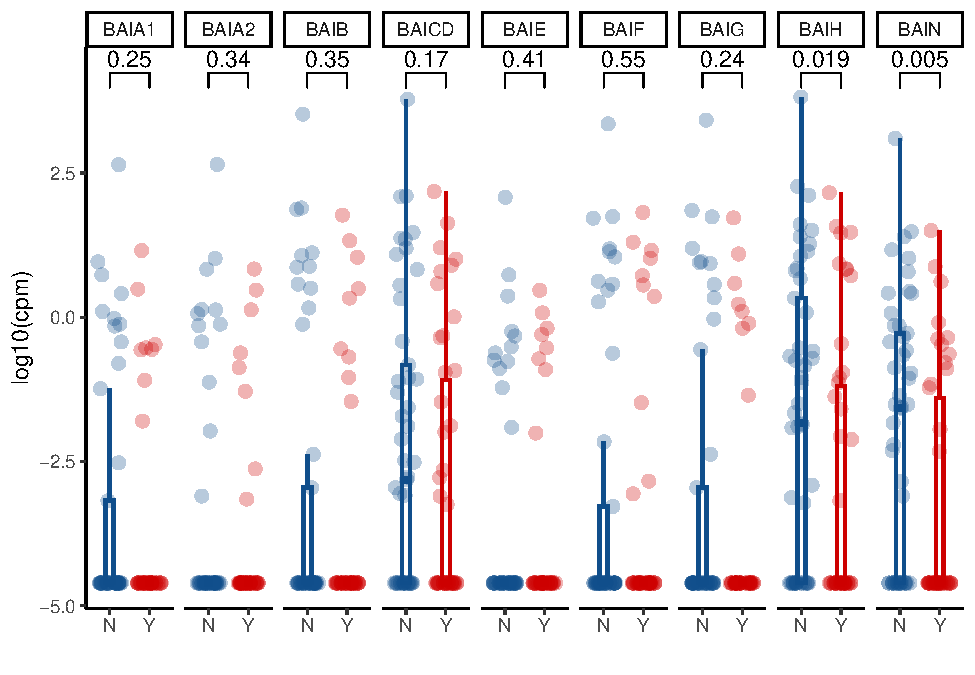
\includegraphics{_main_files/figure-latex/unnamed-chunk-24-1.pdf}

\hypertarget{bile-acid-related-bacteria}{%
\section{Bile acid related bacteria}\label{bile-acid-related-bacteria}}

\hypertarget{eggerthella-lenta}{%
\subsection{Eggerthella lenta}\label{eggerthella-lenta}}

\begin{Shaded}
\begin{Highlighting}[]
\NormalTok{taxa\_bas\_later }\SpecialCharTok{\%\textgreater{}\%} 
  \FunctionTok{ggplot}\NormalTok{(}\FunctionTok{aes}\NormalTok{(}\AttributeTok{x=}\NormalTok{GI\_GVHD, }\AttributeTok{y=}\FunctionTok{log10}\NormalTok{(eggerthella\_lenta}\SpecialCharTok{+} \FloatTok{1.5e{-}08}\NormalTok{), }\AttributeTok{color=}\NormalTok{GI\_GVHD))}\SpecialCharTok{+}
  \FunctionTok{geom\_boxplot}\NormalTok{(}\AttributeTok{width=}\FloatTok{0.2}\NormalTok{, }\AttributeTok{lwd=}\FloatTok{0.8}\NormalTok{, }\AttributeTok{outlier.shape =} \ConstantTok{NA}\NormalTok{) }\SpecialCharTok{+}
  \FunctionTok{geom\_jitter}\NormalTok{(}\AttributeTok{width=}\FloatTok{0.3}\NormalTok{, }\AttributeTok{alpha=}\FloatTok{0.3}\NormalTok{, }\AttributeTok{size=}\FloatTok{2.5}\NormalTok{)}\SpecialCharTok{+}
  \FunctionTok{ylab}\NormalTok{(}\StringTok{"log10(Eggerthella lenta)"}\NormalTok{)}\SpecialCharTok{+}
  \FunctionTok{xlab}\NormalTok{(}\StringTok{""}\NormalTok{)}\SpecialCharTok{+}
  \FunctionTok{theme\_classic}\NormalTok{()}\SpecialCharTok{+}
  \FunctionTok{stat\_compare\_means}\NormalTok{(}\AttributeTok{comparisons=}\FunctionTok{list}\NormalTok{(}\FunctionTok{c}\NormalTok{(}\StringTok{"N"}\NormalTok{, }\StringTok{"Y"}\NormalTok{)),}
                     \AttributeTok{method=}\StringTok{"wilcox.test"}\NormalTok{,}
                     \AttributeTok{correct=}\ConstantTok{FALSE}\NormalTok{)}\SpecialCharTok{+}
  \FunctionTok{scale\_color\_manual}\NormalTok{(}\AttributeTok{values=}\FunctionTok{c}\NormalTok{(}\StringTok{"dodgerblue4"}\NormalTok{, }\StringTok{"red3"}\NormalTok{))}\SpecialCharTok{+}
  \FunctionTok{theme}\NormalTok{(}\AttributeTok{legend.position=}\StringTok{"none"}\NormalTok{)}
\end{Highlighting}
\end{Shaded}

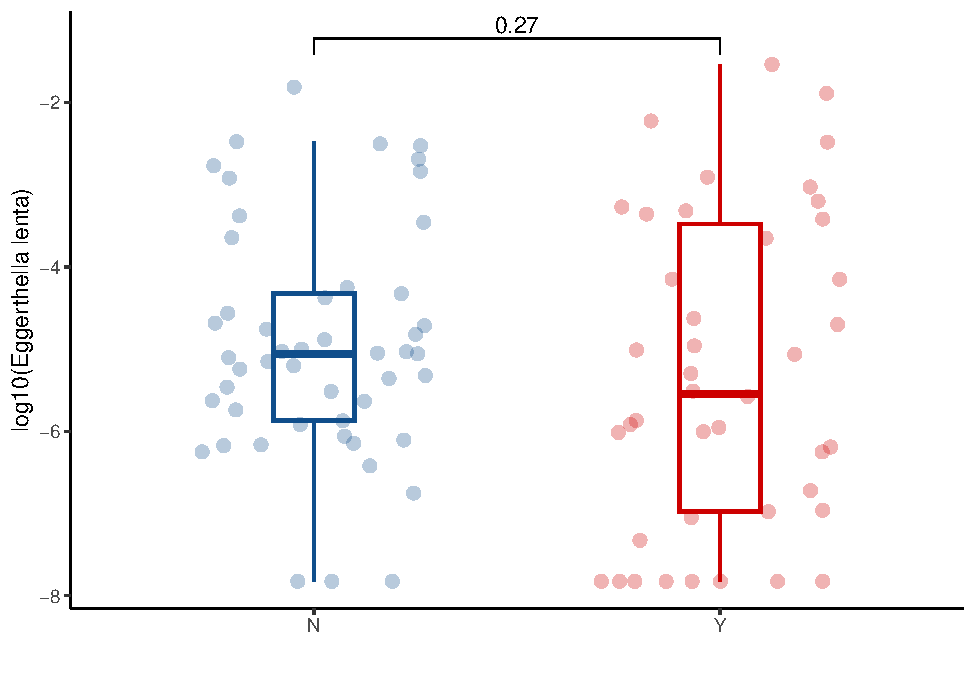
\includegraphics{_main_files/figure-latex/unnamed-chunk-25-1.pdf}

\hypertarget{ruminococcus-gnavus}{%
\subsection{Ruminococcus gnavus}\label{ruminococcus-gnavus}}

\begin{Shaded}
\begin{Highlighting}[]
\NormalTok{taxa\_bas\_later }\SpecialCharTok{\%\textgreater{}\%} 
  \FunctionTok{ggplot}\NormalTok{(}\FunctionTok{aes}\NormalTok{(}\AttributeTok{x=}\NormalTok{GI\_GVHD, }\AttributeTok{y=}\FunctionTok{log10}\NormalTok{(ruminococcus\_gnavus}\SpecialCharTok{+} \FloatTok{1.4e{-}07}\NormalTok{), }\AttributeTok{color=}\NormalTok{GI\_GVHD))}\SpecialCharTok{+}
  \FunctionTok{geom\_boxplot}\NormalTok{(}\AttributeTok{width=}\FloatTok{0.2}\NormalTok{, }\AttributeTok{lwd=}\FloatTok{0.8}\NormalTok{, }\AttributeTok{outlier.shape =} \ConstantTok{NA}\NormalTok{) }\SpecialCharTok{+}
  \FunctionTok{geom\_jitter}\NormalTok{(}\AttributeTok{width=}\FloatTok{0.3}\NormalTok{, }\AttributeTok{alpha=}\FloatTok{0.3}\NormalTok{, }\AttributeTok{size=}\FloatTok{2.5}\NormalTok{)}\SpecialCharTok{+}
  \FunctionTok{ylab}\NormalTok{(}\StringTok{"log10(Ruminococcus gnavus)"}\NormalTok{)}\SpecialCharTok{+}
  \FunctionTok{xlab}\NormalTok{(}\StringTok{""}\NormalTok{)}\SpecialCharTok{+}
  \FunctionTok{theme\_classic}\NormalTok{()}\SpecialCharTok{+}
  \FunctionTok{stat\_compare\_means}\NormalTok{(}\AttributeTok{comparisons=}\FunctionTok{list}\NormalTok{(}\FunctionTok{c}\NormalTok{(}\StringTok{"N"}\NormalTok{, }\StringTok{"Y"}\NormalTok{)),}
                     \AttributeTok{method=}\StringTok{"wilcox.test"}\NormalTok{,}
                     \AttributeTok{correct=}\ConstantTok{FALSE}\NormalTok{)}\SpecialCharTok{+}
  \FunctionTok{scale\_color\_manual}\NormalTok{(}\AttributeTok{values=}\FunctionTok{c}\NormalTok{(}\StringTok{"dodgerblue4"}\NormalTok{, }\StringTok{"red3"}\NormalTok{))}\SpecialCharTok{+}
  \FunctionTok{theme}\NormalTok{(}\AttributeTok{legend.position=}\StringTok{"none"}\NormalTok{)}
\end{Highlighting}
\end{Shaded}

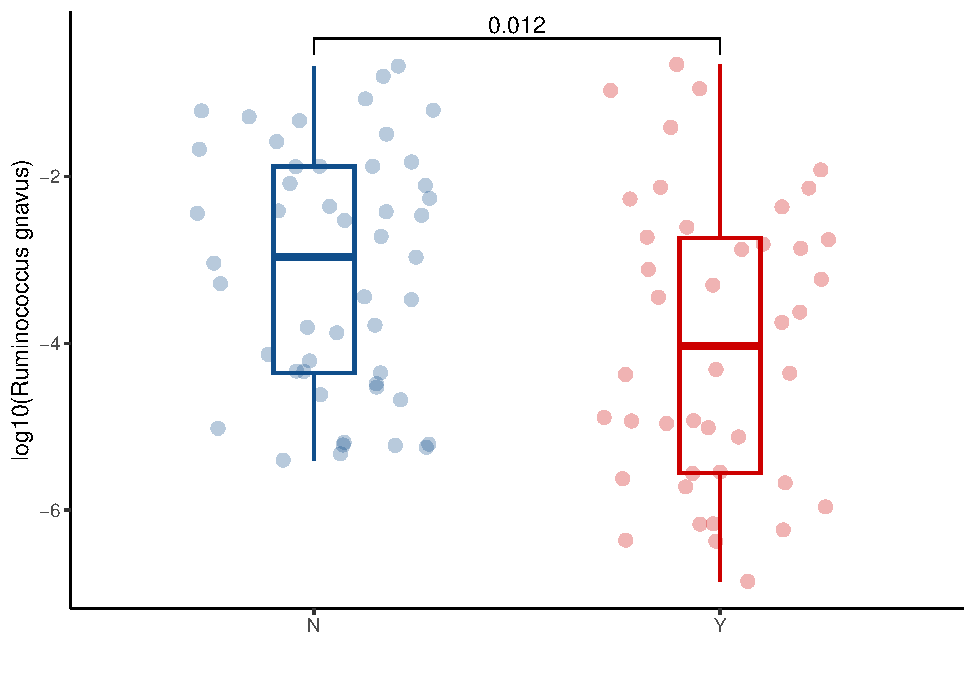
\includegraphics{_main_files/figure-latex/unnamed-chunk-26-1.pdf}

\hypertarget{create-landscape-of-all-peri-gvhd-onset-samples-figure-5}{%
\chapter{Create landscape of all peri-GVHD-onset samples (figure 5)}\label{create-landscape-of-all-peri-gvhd-onset-samples-figure-5}}

\hypertarget{define-sample-order-from-higher-nonudca-secondary-bas-to-lower}{%
\section{Define sample order from higher nonUDCA secondary BAs to lower}\label{define-sample-order-from-higher-nonudca-secondary-bas-to-lower}}

\begin{Shaded}
\begin{Highlighting}[]
\NormalTok{samples\_key}\OtherTok{\textless{}{-}}\NormalTok{BSH\_metalphlan }\SpecialCharTok{\%\textgreater{}\%} \FunctionTok{distinct}\NormalTok{(sampleid) }\SpecialCharTok{\%\textgreater{}\%}  
  \FunctionTok{left\_join}\NormalTok{(later\_pools\_final }\SpecialCharTok{\%\textgreater{}\%} \FunctionTok{select}\NormalTok{(sampleid, secondary\_nonUDCA)) }\SpecialCharTok{\%\textgreater{}\%} 
  \FunctionTok{left\_join}\NormalTok{(cohort\_BAS) }\SpecialCharTok{\%\textgreater{}\%} 
  \FunctionTok{filter}\NormalTok{(later}\SpecialCharTok{==}\StringTok{"Y"}\NormalTok{) }\SpecialCharTok{\%\textgreater{}\%} 
  \FunctionTok{arrange}\NormalTok{(}\FunctionTok{desc}\NormalTok{(secondary\_nonUDCA)) }\SpecialCharTok{\%\textgreater{}\%} 
  \FunctionTok{left\_join}\NormalTok{(ursodiol) }\SpecialCharTok{\%\textgreater{}\%} \FunctionTok{filter}\NormalTok{(ursodiol2}\SpecialCharTok{==}\StringTok{"Y"}\NormalTok{)}

\NormalTok{level\_order }\OtherTok{\textless{}{-}}\NormalTok{ samples\_key}\SpecialCharTok{$}\NormalTok{sampleid}
\end{Highlighting}
\end{Shaded}

\hypertarget{gi-gvhd-plot}{%
\section{GI GVHD plot}\label{gi-gvhd-plot}}

\begin{Shaded}
\begin{Highlighting}[]
\NormalTok{gi\_gvhd\_plot}\OtherTok{\textless{}{-}}\NormalTok{cohort\_BAS }\SpecialCharTok{\%\textgreater{}\%} 
  \FunctionTok{filter}\NormalTok{(later}\SpecialCharTok{==}\StringTok{"Y"}\NormalTok{) }\SpecialCharTok{\%\textgreater{}\%} 
  \FunctionTok{ggplot}\NormalTok{((}\FunctionTok{aes}\NormalTok{(}\AttributeTok{x =} \FunctionTok{factor}\NormalTok{(sampleid, }\AttributeTok{levels =}\NormalTok{ level\_order), }\AttributeTok{y =} \DecValTok{1}\NormalTok{, }\AttributeTok{fill =}\NormalTok{ GI\_GVHD))) }\SpecialCharTok{+} 
  \FunctionTok{geom\_raster}\NormalTok{(}\AttributeTok{color =} \StringTok{"black"}\NormalTok{, }\AttributeTok{size =} \FloatTok{0.5}\NormalTok{) }\SpecialCharTok{+}
  \FunctionTok{theme\_classic}\NormalTok{()}\SpecialCharTok{+} \FunctionTok{theme}\NormalTok{(}\AttributeTok{axis.text.x=}\FunctionTok{element\_blank}\NormalTok{())}\SpecialCharTok{+}
  \FunctionTok{xlab}\NormalTok{(}\StringTok{""}\NormalTok{)}\SpecialCharTok{+}
  \FunctionTok{ylab}\NormalTok{(}\StringTok{""}\NormalTok{)}\SpecialCharTok{+}
  \FunctionTok{scale\_fill\_manual}\NormalTok{(}\AttributeTok{values=}\FunctionTok{c}\NormalTok{(}\StringTok{"white"}\NormalTok{, }\StringTok{"dodgerblue4"}\NormalTok{))}\SpecialCharTok{+}
  \FunctionTok{theme}\NormalTok{(}\AttributeTok{axis.text.y =} \FunctionTok{element\_blank}\NormalTok{())}\SpecialCharTok{+}
  \FunctionTok{theme}\NormalTok{(}\AttributeTok{legend.position =} \StringTok{"none"}\NormalTok{) }\CommentTok{\#only for plotting reasons}
  
\NormalTok{gi\_gvhd\_plot}
\end{Highlighting}
\end{Shaded}

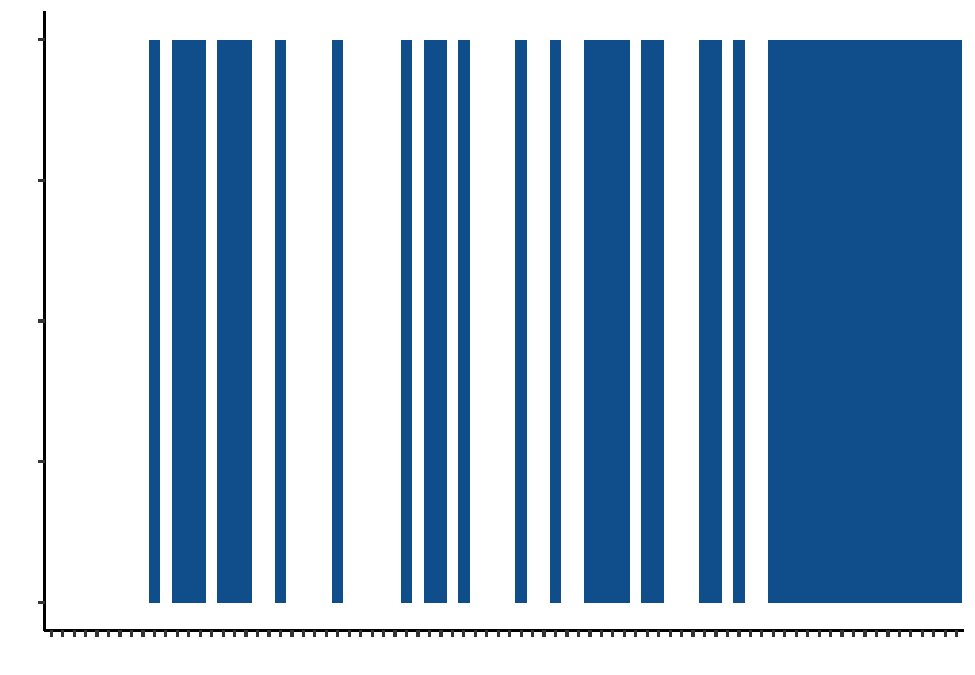
\includegraphics{_main_files/figure-latex/unnamed-chunk-28-1.pdf}

\hypertarget{sba-plot}{%
\section{SBA plot}\label{sba-plot}}

\begin{Shaded}
\begin{Highlighting}[]
\NormalTok{sba\_plot}\OtherTok{\textless{}{-}}\FunctionTok{ggplot}\NormalTok{(samples\_key, }\FunctionTok{aes}\NormalTok{(}\AttributeTok{x=}\FunctionTok{factor}\NormalTok{(sampleid, }\AttributeTok{level=}\NormalTok{level\_order), }\AttributeTok{y=}\FunctionTok{log10}\NormalTok{(secondary\_nonUDCA)))}\SpecialCharTok{+}
  \FunctionTok{geom\_point}\NormalTok{(}\AttributeTok{size=}\DecValTok{3}\NormalTok{)}\SpecialCharTok{+}\FunctionTok{theme\_classic}\NormalTok{()}\SpecialCharTok{+}
  \FunctionTok{ylab}\NormalTok{(}\StringTok{"log(SBAs*)"}\NormalTok{)}\SpecialCharTok{+}
  \FunctionTok{theme}\NormalTok{(}\AttributeTok{axis.text.x=}\FunctionTok{element\_blank}\NormalTok{())}\SpecialCharTok{+}
  \FunctionTok{xlab}\NormalTok{(}\StringTok{""}\NormalTok{)}
\NormalTok{sba\_plot}
\end{Highlighting}
\end{Shaded}

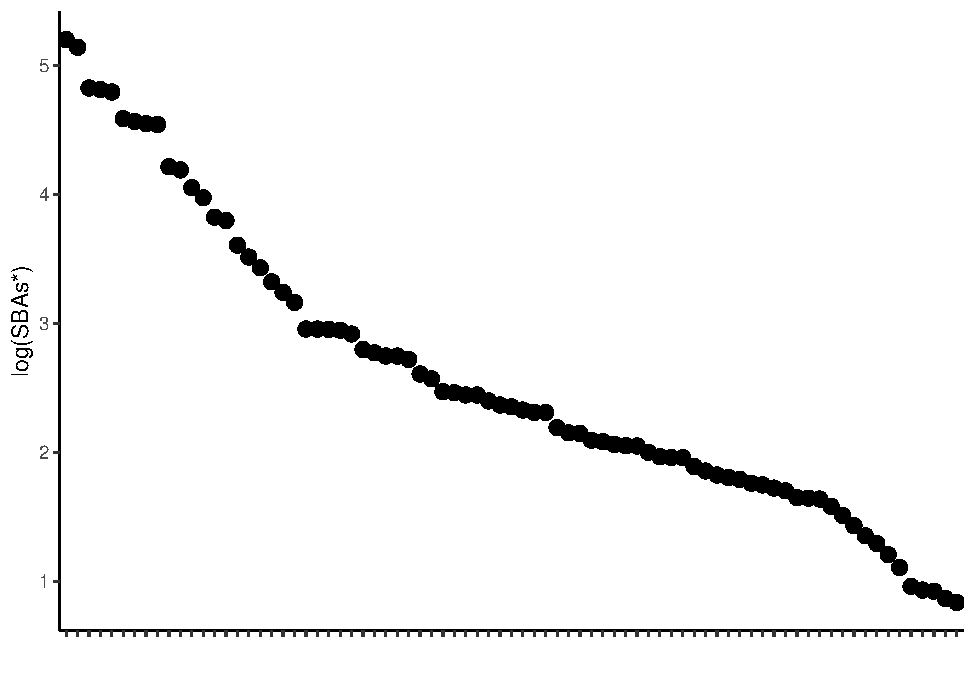
\includegraphics{_main_files/figure-latex/unnamed-chunk-29-1.pdf}

\hypertarget{a-diversity-plot}{%
\section{A-diversity plot}\label{a-diversity-plot}}

\begin{Shaded}
\begin{Highlighting}[]
\NormalTok{adiv\_pre}\OtherTok{\textless{}{-}}\NormalTok{cohort\_BAS }\SpecialCharTok{\%\textgreater{}\%} 
  \FunctionTok{filter}\NormalTok{(later}\SpecialCharTok{==}\StringTok{"Y"}\NormalTok{) }\SpecialCharTok{\%\textgreater{}\%} 
  \FunctionTok{left\_join}\NormalTok{(asv\_alpha\_all) }\SpecialCharTok{\%\textgreater{}\%}  \CommentTok{\#add a{-}diversity}
  \FunctionTok{inner\_join}\NormalTok{(samples\_key) }\SpecialCharTok{\%\textgreater{}\%} 
  \FunctionTok{arrange}\NormalTok{(}\FunctionTok{desc}\NormalTok{(secondary\_nonUDCA)) }\SpecialCharTok{\%\textgreater{}\%}
          \FunctionTok{mutate}\NormalTok{(}\AttributeTok{rank =} \DecValTok{1}\SpecialCharTok{:}\FunctionTok{nrow}\NormalTok{(.))}

\NormalTok{adiv\_plot}\OtherTok{\textless{}{-}}\FunctionTok{ggplot}\NormalTok{(adiv\_pre, }\FunctionTok{aes}\NormalTok{(}\AttributeTok{x =}\NormalTok{ rank, }\AttributeTok{y =}\NormalTok{ simpson\_reciprocal)) }\SpecialCharTok{+}
  \FunctionTok{geom\_point}\NormalTok{(}\AttributeTok{size=}\DecValTok{3}\NormalTok{) }\SpecialCharTok{+}
  \FunctionTok{geom\_smooth}\NormalTok{(}\AttributeTok{method =} \StringTok{"loess"}\NormalTok{) }\SpecialCharTok{+}
  \FunctionTok{theme\_classic}\NormalTok{() }\SpecialCharTok{+}
  \FunctionTok{ylab}\NormalTok{(}\StringTok{"a{-}diversity"}\NormalTok{) }\SpecialCharTok{+}
  \CommentTok{\#xlab("sampleid") +}
  \FunctionTok{theme}\NormalTok{(}\AttributeTok{axis.text.x =} \FunctionTok{element\_blank}\NormalTok{()) }\SpecialCharTok{+}
  \FunctionTok{xlab}\NormalTok{(}\StringTok{""}\NormalTok{) }\SpecialCharTok{+}
  \FunctionTok{scale\_x\_discrete}\NormalTok{(}\AttributeTok{limits =}\NormalTok{ adiv\_pre}\SpecialCharTok{$}\NormalTok{rank[}\FunctionTok{order}\NormalTok{(}\SpecialCharTok{{-}}\NormalTok{adiv\_pre}\SpecialCharTok{$}\NormalTok{rank)])}

\NormalTok{adiv\_plot}
\end{Highlighting}
\end{Shaded}

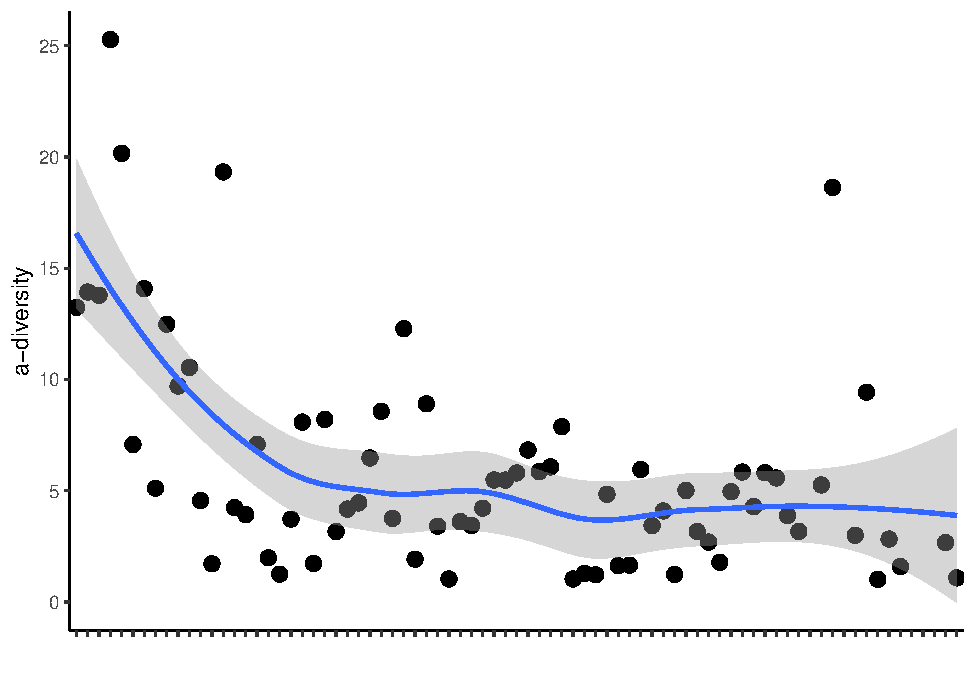
\includegraphics{_main_files/figure-latex/unnamed-chunk-30-1.pdf}

\hypertarget{bile-acid-related-genes}{%
\section{Bile acid related genes}\label{bile-acid-related-genes}}

\begin{Shaded}
\begin{Highlighting}[]
\NormalTok{bai\_genes\_clean}\SpecialCharTok{$}\NormalTok{sampleid }\OtherTok{\textless{}{-}}\FunctionTok{gsub}\NormalTok{(}\StringTok{"FMT\_"}\NormalTok{, }\StringTok{"FMT."}\NormalTok{, bai\_genes\_clean}\SpecialCharTok{$}\NormalTok{sampleid)}

\NormalTok{ba\_genes\_pre}\OtherTok{\textless{}{-}}\NormalTok{samples\_key }\SpecialCharTok{\%\textgreater{}\%} 
  \FunctionTok{select}\NormalTok{(sampleid, GI\_GVHD, secondary\_nonUDCA) }\SpecialCharTok{\%\textgreater{}\%} 
  \FunctionTok{left\_join}\NormalTok{(BSH\_metalphlan }\SpecialCharTok{\%\textgreater{}\%} 
              \FunctionTok{select}\NormalTok{(sampleid, cpm, KOID)) }\SpecialCharTok{\%\textgreater{}\%} 
  \FunctionTok{rename}\NormalTok{(}\AttributeTok{gene=}\NormalTok{KOID) }\SpecialCharTok{\%\textgreater{}\%} 
  \FunctionTok{mutate}\NormalTok{(}\AttributeTok{gene=}\FunctionTok{ifelse}\NormalTok{(gene}\SpecialCharTok{==}\StringTok{"K01442"}\NormalTok{, }\StringTok{"BSH"}\NormalTok{, }\ConstantTok{NA}\NormalTok{)) }\SpecialCharTok{\%\textgreater{}\%} 
  \FunctionTok{distinct}\NormalTok{() }\SpecialCharTok{\%\textgreater{}\%} 
  \FunctionTok{spread}\NormalTok{(}\AttributeTok{key=}\NormalTok{gene, }\AttributeTok{value=}\NormalTok{cpm, }\AttributeTok{fill=}\DecValTok{0}\NormalTok{)}
  
\NormalTok{operon\_genes\_pre}\OtherTok{\textless{}{-}}\NormalTok{samples\_key }\SpecialCharTok{\%\textgreater{}\%}
  \FunctionTok{left\_join}\NormalTok{(bai\_genes\_clean) }\SpecialCharTok{\%\textgreater{}\%} 
  \FunctionTok{select}\NormalTok{(sampleid, cpm, gene) }\SpecialCharTok{\%\textgreater{}\%} 
  \FunctionTok{distinct}\NormalTok{() }\SpecialCharTok{\%\textgreater{}\%} 
  \FunctionTok{spread}\NormalTok{(}\AttributeTok{key=}\NormalTok{gene, }\AttributeTok{value=}\NormalTok{cpm, }\AttributeTok{fill=}\DecValTok{0}\NormalTok{)}

\NormalTok{pre\_bai\_plot}\OtherTok{\textless{}{-}}\NormalTok{ba\_genes\_pre }\SpecialCharTok{\%\textgreater{}\%} 
  \FunctionTok{left\_join}\NormalTok{(operon\_genes\_pre) }\SpecialCharTok{\%\textgreater{}\%} 
  \FunctionTok{select}\NormalTok{(}\SpecialCharTok{{-}}\NormalTok{GI\_GVHD, }\SpecialCharTok{{-}}\NormalTok{secondary\_nonUDCA) }\SpecialCharTok{\%\textgreater{}\%} 
  \FunctionTok{gather}\NormalTok{(}\StringTok{"gene"}\NormalTok{, }\StringTok{"cpm"}\NormalTok{, }\FunctionTok{names}\NormalTok{(.)[}\DecValTok{2}\NormalTok{]}\SpecialCharTok{:}\FunctionTok{names}\NormalTok{(.)[}\FunctionTok{ncol}\NormalTok{(.)]) }


\NormalTok{bai\_plot}\OtherTok{\textless{}{-}}\NormalTok{pre\_bai\_plot }\SpecialCharTok{\%\textgreater{}\%} 
  \FunctionTok{ggplot}\NormalTok{(}\FunctionTok{aes}\NormalTok{(}\AttributeTok{x=}\FunctionTok{factor}\NormalTok{(sampleid, }\AttributeTok{level=}\NormalTok{level\_order), }\AttributeTok{y=}\NormalTok{gene, }\AttributeTok{fill=}\FunctionTok{log10}\NormalTok{(cpm}\FloatTok{+0.05}\NormalTok{)))}\SpecialCharTok{+}
           \FunctionTok{geom\_tile}\NormalTok{()}\SpecialCharTok{+}
  \FunctionTok{xlab}\NormalTok{(}\StringTok{""}\NormalTok{)}\SpecialCharTok{+}
  \FunctionTok{ylab}\NormalTok{(}\StringTok{"bile acid genes"}\NormalTok{)}\SpecialCharTok{+}
  \FunctionTok{scale\_fill\_gradient}\NormalTok{(}\AttributeTok{low=}\StringTok{"white"}\NormalTok{, }\AttributeTok{high=}\StringTok{"red"}\NormalTok{)}\SpecialCharTok{+}
  \FunctionTok{theme}\NormalTok{(}\AttributeTok{axis.text.x=}\FunctionTok{element\_blank}\NormalTok{())}\SpecialCharTok{+}
  \FunctionTok{theme}\NormalTok{(}\AttributeTok{legend.position =} \StringTok{"none"}\NormalTok{) }\CommentTok{\#only for plotting reasons}
\NormalTok{bai\_plot}
\end{Highlighting}
\end{Shaded}

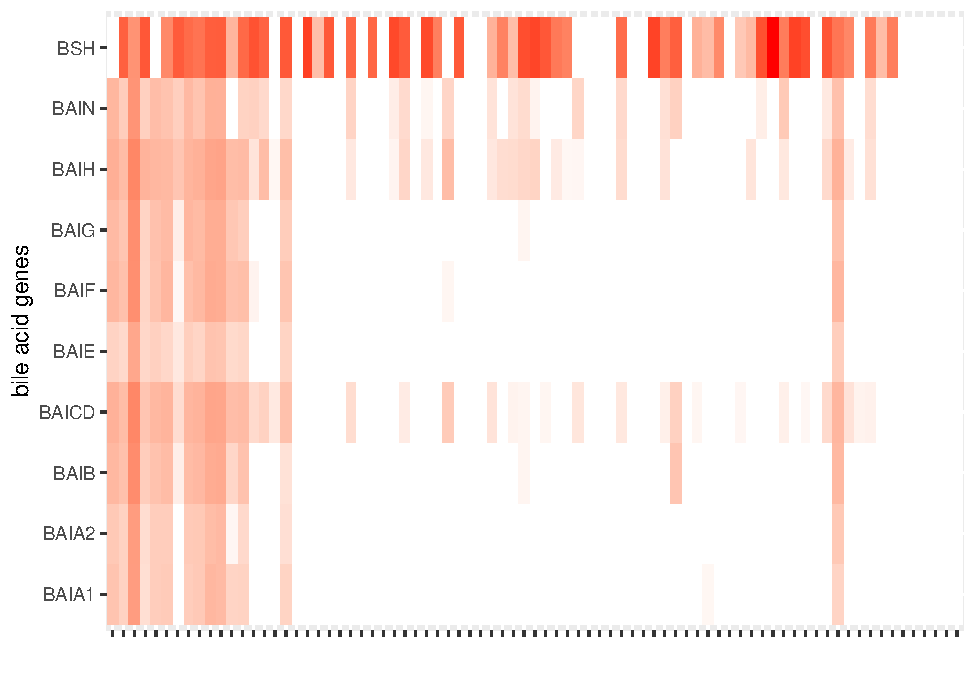
\includegraphics{_main_files/figure-latex/unnamed-chunk-31-1.pdf}

\hypertarget{microbiome-composition}{%
\section{Microbiome composition}\label{microbiome-composition}}

\begin{Shaded}
\begin{Highlighting}[]
\FunctionTok{setDT}\NormalTok{(asv\_annotation\_blast\_color\_ag)}
\NormalTok{asv\_color\_base\_set }\OtherTok{=} \FunctionTok{unique}\NormalTok{(asv\_annotation\_blast\_color\_ag[,.(color\_label\_group,color\_base)])}
\NormalTok{color\_base\_set\_asv\_carT }\OtherTok{=}\NormalTok{ asv\_color\_base\_set}\SpecialCharTok{$}\NormalTok{color\_base}
\FunctionTok{names}\NormalTok{(color\_base\_set\_asv\_carT) }\OtherTok{=}\NormalTok{asv\_color\_base\_set}\SpecialCharTok{$}\NormalTok{color\_label\_group;}
\NormalTok{gg }\OtherTok{=} \FunctionTok{ggplot}\NormalTok{(asv\_color\_base\_set, }\FunctionTok{aes}\NormalTok{(color\_label\_group,}\AttributeTok{y=}\DecValTok{1}\NormalTok{,}\AttributeTok{fill=}\NormalTok{color\_label\_group)) }\SpecialCharTok{+} \FunctionTok{geom\_tile}\NormalTok{()  }\SpecialCharTok{+}
  \FunctionTok{scale\_fill\_manual}\NormalTok{(}\AttributeTok{values =}\NormalTok{ color\_base\_set\_asv\_carT) }\SpecialCharTok{+}
  \FunctionTok{theme\_classic}\NormalTok{() }\SpecialCharTok{+}
  \FunctionTok{theme}\NormalTok{(}\AttributeTok{axis.text.x =} \FunctionTok{element\_text}\NormalTok{(}\AttributeTok{angle=}\DecValTok{60}\NormalTok{,}\AttributeTok{hjust =} \DecValTok{1}\NormalTok{)) }\SpecialCharTok{+}
  \FunctionTok{theme}\NormalTok{(}\AttributeTok{legend.position =} \StringTok{"none"}\NormalTok{)}

\CommentTok{\#color\_set\_asv\_carT maps each distinct taxonomic group to its corresponding color.}
\NormalTok{asv\_color\_set }\OtherTok{=} \FunctionTok{unique}\NormalTok{(asv\_annotation\_blast\_color\_ag[,.(color,color\_label\_group\_distinct,color\_label\_group,color\_base)])}
\NormalTok{color\_set\_asv\_carT }\OtherTok{=}\NormalTok{ asv\_color\_set}\SpecialCharTok{$}\NormalTok{color}
\FunctionTok{names}\NormalTok{(color\_set\_asv\_carT) }\OtherTok{=}\NormalTok{asv\_color\_set}\SpecialCharTok{$}\NormalTok{color\_label\_group\_distinct;}
\FunctionTok{setDT}\NormalTok{(counts\_samples)}
\FunctionTok{setDT}\NormalTok{(asv\_annotation\_blast\_color\_ag)}
\NormalTok{m }\OtherTok{=} \FunctionTok{merge}\NormalTok{(counts\_samples[,.(asv\_key,sampleid,}
\NormalTok{                         count,count\_relative,count\_total)],}
\NormalTok{          asv\_annotation\_blast\_color\_ag[,.(asv\_key,color\_label\_group\_distinct)]);}

\NormalTok{sample\_composition }\OtherTok{\textless{}{-}}\NormalTok{ m }\SpecialCharTok{\%\textgreater{}\%} 
  \FunctionTok{left\_join}\NormalTok{(cohort\_BAS }\SpecialCharTok{\%\textgreater{}\%} \FunctionTok{select}\NormalTok{(PID, sampleid)) }\SpecialCharTok{\%\textgreater{}\%} 
  \FunctionTok{left\_join}\NormalTok{(cohort\_BAS) }\SpecialCharTok{\%\textgreater{}\%} 
  \FunctionTok{filter}\NormalTok{(later}\SpecialCharTok{==}\StringTok{"Y"}\NormalTok{)}


\NormalTok{m1}\OtherTok{\textless{}{-}}\NormalTok{sample\_composition }\SpecialCharTok{\%\textgreater{}\%} 
  \FunctionTok{group\_by}\NormalTok{(sampleid, color\_label\_group\_distinct) }\SpecialCharTok{\%\textgreater{}\%} 
  \FunctionTok{inner\_join}\NormalTok{(samples\_key) }\SpecialCharTok{\%\textgreater{}\%} 
  \FunctionTok{mutate}\NormalTok{(}\AttributeTok{sampleid =} \FunctionTok{fct\_reorder}\NormalTok{(sampleid, }\FunctionTok{desc}\NormalTok{(secondary\_nonUDCA))) }

\NormalTok{m1}\SpecialCharTok{$}\NormalTok{color\_label\_group\_distinct }\OtherTok{=} \FunctionTok{factor}\NormalTok{(m1}\SpecialCharTok{$}\NormalTok{color\_label\_group\_distinct,}\AttributeTok{levels =} \FunctionTok{sort}\NormalTok{(}\FunctionTok{unique}\NormalTok{(m1}\SpecialCharTok{$}\NormalTok{color\_label\_group\_distinct),}\AttributeTok{decreasing =}\NormalTok{ T));}
\NormalTok{gg\_composition }\OtherTok{=} \FunctionTok{ggplot}\NormalTok{(m1,}
                        \FunctionTok{aes}\NormalTok{(}\AttributeTok{x=}\FunctionTok{factor}\NormalTok{(sampleid, }\AttributeTok{levels=}\NormalTok{level\_order),}
                            \AttributeTok{y=}\NormalTok{count\_relative,}
                            \AttributeTok{fill=}\NormalTok{color\_label\_group\_distinct) ) }\SpecialCharTok{+}
  \FunctionTok{geom\_bar}\NormalTok{(}\AttributeTok{stat =} \StringTok{"identity"}\NormalTok{,}\AttributeTok{position=}\StringTok{"fill"}\NormalTok{,}\AttributeTok{width =} \DecValTok{1}\NormalTok{) }\SpecialCharTok{+}
  \FunctionTok{theme\_classic}\NormalTok{() }\SpecialCharTok{+}
  \FunctionTok{theme}\NormalTok{(}\AttributeTok{axis.text.x =} \FunctionTok{element\_blank}\NormalTok{(),}
        \AttributeTok{axis.text.y =} \FunctionTok{element\_blank}\NormalTok{(),}
        \AttributeTok{legend.position =} \StringTok{"none"}\NormalTok{) }\SpecialCharTok{+}
  \FunctionTok{xlab}\NormalTok{(}\StringTok{""}\NormalTok{)}\SpecialCharTok{+}
  \FunctionTok{scale\_fill\_manual}\NormalTok{(}\AttributeTok{values =}\NormalTok{ color\_set\_asv\_carT);}
\FunctionTok{print}\NormalTok{(gg\_composition)}
\end{Highlighting}
\end{Shaded}

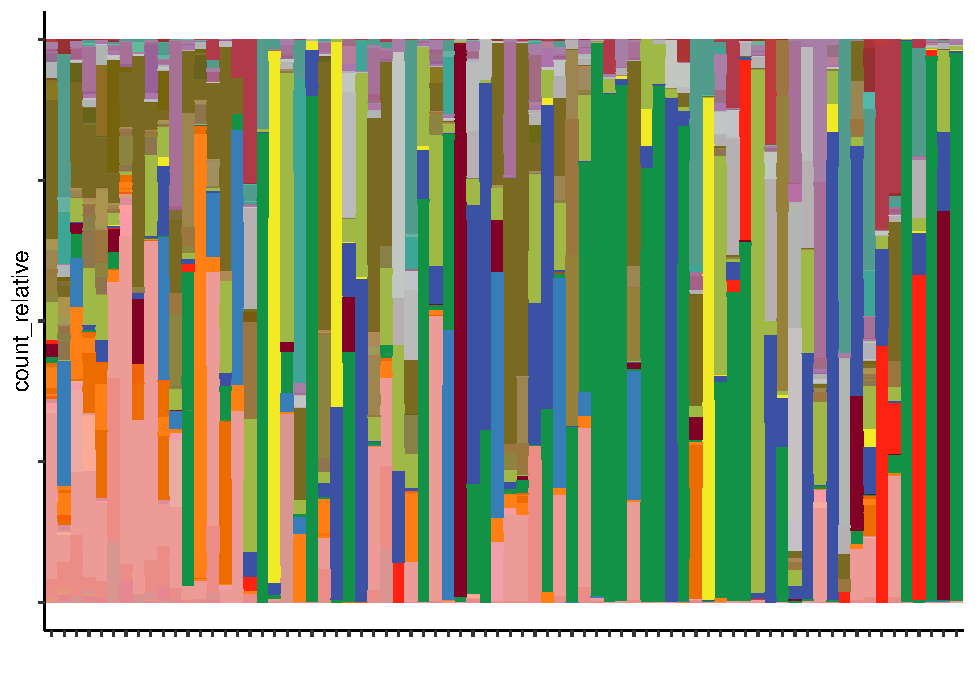
\includegraphics{_main_files/figure-latex/unnamed-chunk-32-1.pdf}

\hypertarget{add-all-plots-together}{%
\section{Add all plots together}\label{add-all-plots-together}}

\begin{Shaded}
\begin{Highlighting}[]
\FunctionTok{library}\NormalTok{(cowplot)}
\NormalTok{last}\OtherTok{\textless{}{-}}\FunctionTok{plot\_grid}\NormalTok{(gi\_gvhd\_plot, sba\_plot, bai\_plot, adiv\_plot, gg\_composition, }
          \CommentTok{\#labels = c("A", "B", "C", "D", "E"),}
          \AttributeTok{ncol =} \DecValTok{1}\NormalTok{, }\AttributeTok{nrow =} \DecValTok{5}\NormalTok{,}
          \AttributeTok{align =} \StringTok{"v"}\NormalTok{,}\AttributeTok{axis =} \StringTok{\textquotesingle{}l\textquotesingle{}}\NormalTok{,}
          \AttributeTok{width =} \DecValTok{40}\NormalTok{, }\AttributeTok{height =} \DecValTok{20}\NormalTok{,}
          \AttributeTok{rel\_heights =} \FunctionTok{c}\NormalTok{(}\FloatTok{1.8}\NormalTok{, }\DecValTok{4}\NormalTok{ ,}\DecValTok{6}\NormalTok{, }\DecValTok{6}\NormalTok{, }\DecValTok{10}\NormalTok{))}
\NormalTok{last}
\end{Highlighting}
\end{Shaded}

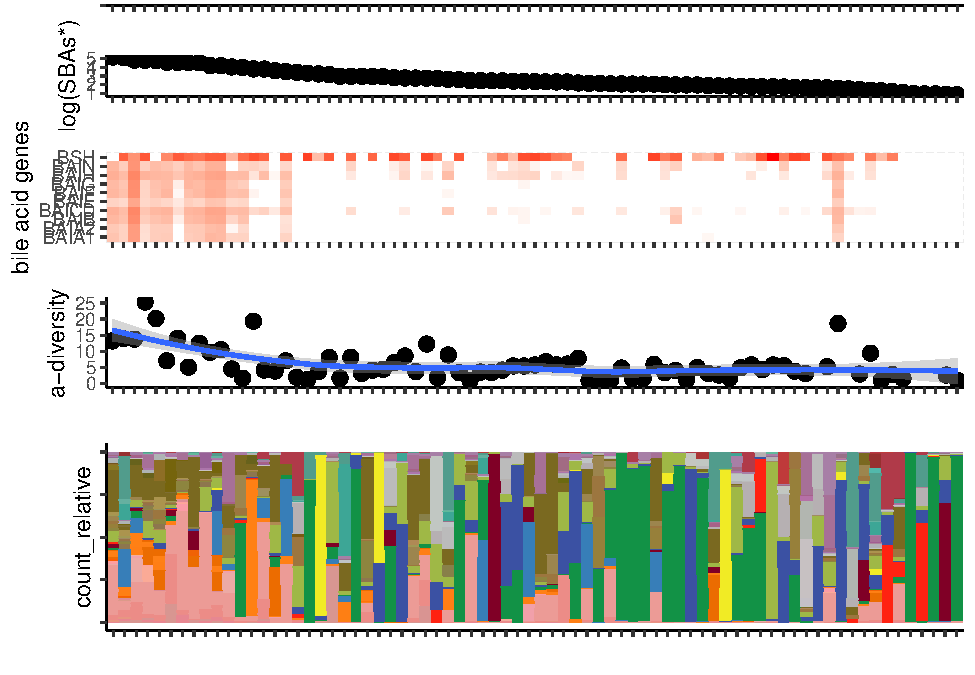
\includegraphics{_main_files/figure-latex/unnamed-chunk-33-1.pdf}

\hypertarget{diversity-bai-operon-and-domination}{%
\chapter{Diversity, bai operon and domination}\label{diversity-bai-operon-and-domination}}

\hypertarget{evaluate-correlation-of-a-diversity-and-bai-operon-sum}{%
\section{Evaluate correlation of a-diversity and bai operon sum}\label{evaluate-correlation-of-a-diversity-and-bai-operon-sum}}

\begin{Shaded}
\begin{Highlighting}[]
\NormalTok{data\_ba}\OtherTok{\textless{}{-}}\NormalTok{ asv\_alpha\_all }\SpecialCharTok{\%\textgreater{}\%}  
  \FunctionTok{inner\_join}\NormalTok{(bai\_genes\_clean }\SpecialCharTok{\%\textgreater{}\%} \FunctionTok{distinct}\NormalTok{(sampleid, bai\_operon\_sum)) }\SpecialCharTok{\%\textgreater{}\%} 
  \FunctionTok{left\_join}\NormalTok{(cohort\_BAS) }\SpecialCharTok{\%\textgreater{}\%} 
  \FunctionTok{filter}\NormalTok{(ursodiol}\SpecialCharTok{==}\StringTok{"Y"}\NormalTok{)}

\NormalTok{data\_ba }\SpecialCharTok{\%\textgreater{}\%} 
\FunctionTok{ggplot}\NormalTok{(}\FunctionTok{aes}\NormalTok{(}\AttributeTok{x=}\FunctionTok{log10}\NormalTok{(simpson\_reciprocal), }\AttributeTok{y=}\FunctionTok{log10}\NormalTok{(bai\_operon\_sum}\FloatTok{+0.01}\NormalTok{)))}\SpecialCharTok{+}
  \FunctionTok{geom\_point}\NormalTok{(}\AttributeTok{alpha=}\FloatTok{0.6}\NormalTok{)}\SpecialCharTok{+}
  \FunctionTok{stat\_cor}\NormalTok{(}\AttributeTok{method=}\StringTok{"pearson"}\NormalTok{)}\SpecialCharTok{+}
  \FunctionTok{geom\_smooth}\NormalTok{(}\AttributeTok{method=}\StringTok{"lm"}\NormalTok{)}\SpecialCharTok{+}
  \FunctionTok{theme\_classic}\NormalTok{()}\SpecialCharTok{+}
  \FunctionTok{ylab}\NormalTok{(}\StringTok{"bai operon log10(cpm)"}\NormalTok{)}\SpecialCharTok{+}
  \FunctionTok{xlab}\NormalTok{(}\StringTok{"a{-}diversity"}\NormalTok{)}
\end{Highlighting}
\end{Shaded}

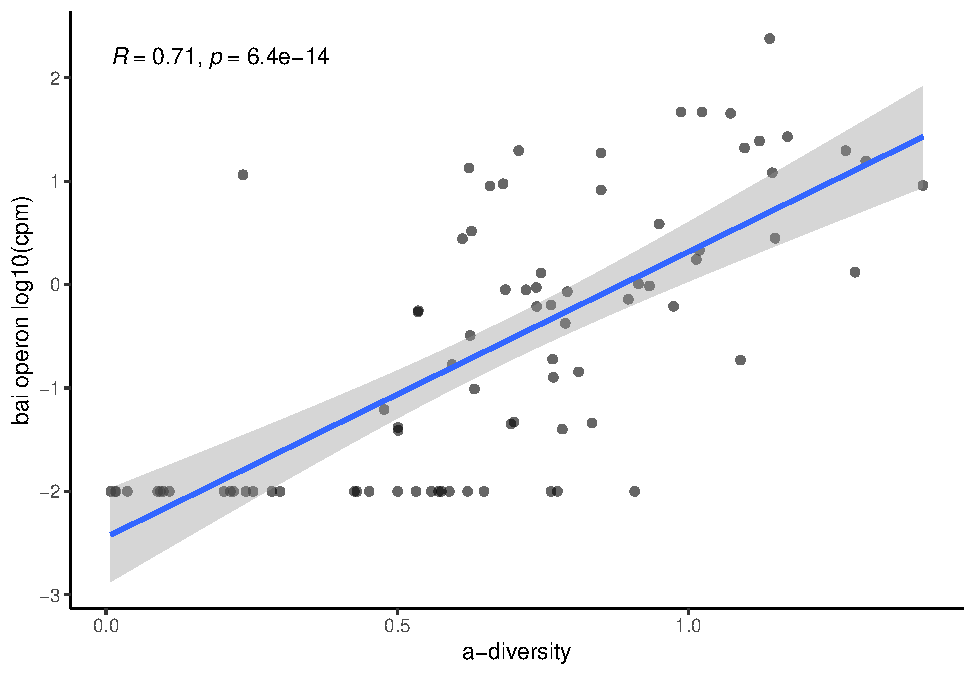
\includegraphics{_main_files/figure-latex/unnamed-chunk-34-1.pdf}

\hypertarget{identify-patients-with-monodomination-by-16s}{%
\section{Identify patients with monodomination by 16S}\label{identify-patients-with-monodomination-by-16s}}

\begin{Shaded}
\begin{Highlighting}[]
\CommentTok{\#create dataset with asv}
\NormalTok{samples\_asv}\OtherTok{\textless{}{-}}\NormalTok{cohort\_BAS }\SpecialCharTok{\%\textgreater{}\%} 
  \FunctionTok{filter}\NormalTok{(later}\SpecialCharTok{==}\StringTok{"Y"}\NormalTok{) }\SpecialCharTok{\%\textgreater{}\%} 
  \FunctionTok{select}\NormalTok{(sampleid) }\SpecialCharTok{\%\textgreater{}\%} 
  \FunctionTok{inner\_join}\NormalTok{(counts\_samples }\SpecialCharTok{\%\textgreater{}\%} 
               \FunctionTok{select}\NormalTok{(sampleid, asv\_key, count, count\_total)) }\SpecialCharTok{\%\textgreater{}\%} 
  \FunctionTok{inner\_join}\NormalTok{(asv\_annotation\_blast\_ag }\SpecialCharTok{\%\textgreater{}\%} 
               \FunctionTok{select}\NormalTok{(asv\_key, kingdom, phylum, class, ordr, family, genus)) }\SpecialCharTok{\%\textgreater{}\%}
  \FunctionTok{mutate}\NormalTok{(}\AttributeTok{relab=}\NormalTok{count}\SpecialCharTok{/}\NormalTok{count\_total) }\SpecialCharTok{\%\textgreater{}\%} 
  \FunctionTok{group\_by}\NormalTok{(sampleid, genus)}

\NormalTok{pathogens\_pre}\OtherTok{\textless{}{-}}\NormalTok{ samples\_asv }\SpecialCharTok{\%\textgreater{}\%} 
  \FunctionTok{filter}\NormalTok{(genus}\SpecialCharTok{==}\StringTok{"Enterococcus"}\SpecialCharTok{|}\NormalTok{genus}\SpecialCharTok{==}\StringTok{"Streptococcus"}\SpecialCharTok{|}\NormalTok{phylum}\SpecialCharTok{==}\StringTok{"Proteobacteria"}\NormalTok{) }\SpecialCharTok{\%\textgreater{}\%} 
  \FunctionTok{mutate}\NormalTok{(}\AttributeTok{enterococcus=}\FunctionTok{ifelse}\NormalTok{(genus}\SpecialCharTok{==}\StringTok{"Enterococcus"}\NormalTok{, relab, }\DecValTok{0}\NormalTok{)) }\SpecialCharTok{\%\textgreater{}\%} 
  \FunctionTok{mutate}\NormalTok{(}\AttributeTok{streptococcus=}\FunctionTok{ifelse}\NormalTok{(genus}\SpecialCharTok{==}\StringTok{"Streptococcus"}\NormalTok{, relab, }\DecValTok{0}\NormalTok{)) }\SpecialCharTok{\%\textgreater{}\%} 
  \FunctionTok{mutate}\NormalTok{(}\AttributeTok{proteobacteria=}\FunctionTok{ifelse}\NormalTok{(phylum}\SpecialCharTok{==}\StringTok{"Proteobacteria"}\NormalTok{, relab, }\DecValTok{0}\NormalTok{)) }\SpecialCharTok{\%\textgreater{}\%} 
  \FunctionTok{mutate}\NormalTok{(}\AttributeTok{enterococcus\_dom=}\FunctionTok{ifelse}\NormalTok{(enterococcus}\SpecialCharTok{\textgreater{}=}\FloatTok{0.3}\NormalTok{, }\StringTok{"Y"}\NormalTok{, }\StringTok{"N"}\NormalTok{)) }\SpecialCharTok{\%\textgreater{}\%} 
  \FunctionTok{mutate}\NormalTok{(}\AttributeTok{streptococcus\_dom=}\FunctionTok{ifelse}\NormalTok{(streptococcus}\SpecialCharTok{\textgreater{}=}\FloatTok{0.3}\NormalTok{, }\StringTok{"Y"}\NormalTok{, }\StringTok{"N"}\NormalTok{)) }\SpecialCharTok{\%\textgreater{}\%} 
   \FunctionTok{mutate}\NormalTok{(}\AttributeTok{proteobacteria\_dom=}\FunctionTok{ifelse}\NormalTok{(proteobacteria}\SpecialCharTok{\textgreater{}=}\FloatTok{0.3}\NormalTok{, }\StringTok{"Y"}\NormalTok{, }\StringTok{"N"}\NormalTok{)) }\SpecialCharTok{\%\textgreater{}\%} 
  \FunctionTok{mutate}\NormalTok{(}\AttributeTok{any\_dom=}\FunctionTok{ifelse}\NormalTok{(enterococcus\_dom}\SpecialCharTok{==}\StringTok{"Y"}\SpecialCharTok{|}\NormalTok{streptococcus\_dom}\SpecialCharTok{==}\StringTok{"Y"}\SpecialCharTok{|}\NormalTok{proteobacteria\_dom}\SpecialCharTok{==}\StringTok{"Y"}\NormalTok{, }\StringTok{"Y"}\NormalTok{, }\StringTok{"N"}\NormalTok{)) }\SpecialCharTok{\%\textgreater{}\%} 
  \FunctionTok{group\_by}\NormalTok{(sampleid) }\SpecialCharTok{\%\textgreater{}\%} 
  \FunctionTok{arrange}\NormalTok{(}\FunctionTok{desc}\NormalTok{(any\_dom)) }\SpecialCharTok{\%\textgreater{}\%} \FunctionTok{slice}\NormalTok{(}\DecValTok{1}\NormalTok{)}
\end{Highlighting}
\end{Shaded}

\hypertarget{domination-and-a-diversity}{%
\section{Domination and a-diversity}\label{domination-and-a-diversity}}

\begin{Shaded}
\begin{Highlighting}[]
\NormalTok{pathogens\_pre }\SpecialCharTok{\%\textgreater{}\%} \FunctionTok{inner\_join}\NormalTok{(asv\_alpha\_all) }\SpecialCharTok{\%\textgreater{}\%} 
  \FunctionTok{ggplot}\NormalTok{(}\FunctionTok{aes}\NormalTok{(}\AttributeTok{x=}\NormalTok{any\_dom, }\AttributeTok{y=}\NormalTok{simpson\_reciprocal, }\AttributeTok{color=}\NormalTok{any\_dom))}\SpecialCharTok{+}
   \FunctionTok{geom\_boxplot}\NormalTok{(}\AttributeTok{width=}\FloatTok{0.2}\NormalTok{, }\AttributeTok{lwd=}\FloatTok{0.8}\NormalTok{, }\AttributeTok{outlier.shape =} \ConstantTok{NA}\NormalTok{) }\SpecialCharTok{+}
  \FunctionTok{geom\_jitter}\NormalTok{(}\AttributeTok{width=}\FloatTok{0.3}\NormalTok{, }\AttributeTok{alpha=}\FloatTok{0.3}\NormalTok{, }\AttributeTok{size=}\FloatTok{2.5}\NormalTok{)}\SpecialCharTok{+}
  \FunctionTok{ylab}\NormalTok{(}\StringTok{"log10(a{-}div)"}\NormalTok{)}\SpecialCharTok{+}
  \FunctionTok{xlab}\NormalTok{(}\StringTok{"domination"}\NormalTok{)}\SpecialCharTok{+}
  \FunctionTok{theme\_classic}\NormalTok{()}\SpecialCharTok{+}
  \FunctionTok{stat\_compare\_means}\NormalTok{(}\AttributeTok{comparisons=}\FunctionTok{list}\NormalTok{(}\FunctionTok{c}\NormalTok{(}\StringTok{"Y"}\NormalTok{, }\StringTok{"N"}\NormalTok{)),}
                     \AttributeTok{method=}\StringTok{"wilcox.test"}\NormalTok{,}
                     \AttributeTok{correct=}\ConstantTok{FALSE}\NormalTok{)}\SpecialCharTok{+}
  \FunctionTok{scale\_color\_manual}\NormalTok{(}\AttributeTok{values=}\FunctionTok{c}\NormalTok{(}\StringTok{"turquoise4"}\NormalTok{,}\StringTok{"darkviolet"}\NormalTok{))}\SpecialCharTok{+}
  \FunctionTok{theme}\NormalTok{(}\AttributeTok{legend.position=}\StringTok{"none"}\NormalTok{)}
\end{Highlighting}
\end{Shaded}

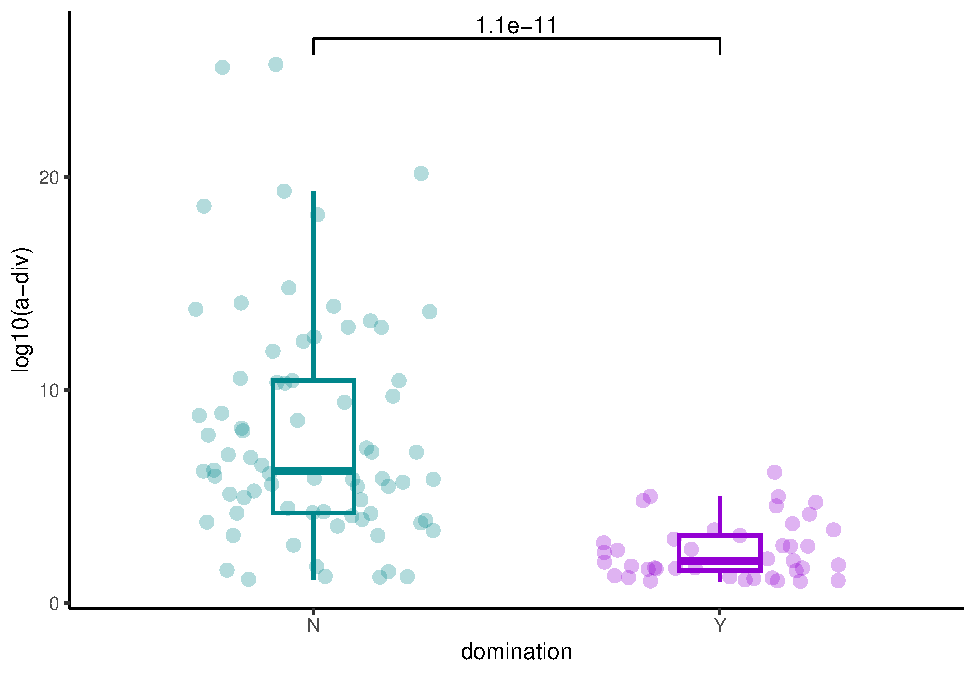
\includegraphics{_main_files/figure-latex/unnamed-chunk-36-1.pdf}

\hypertarget{domination-and-bai-operon}{%
\section{Domination and bai operon}\label{domination-and-bai-operon}}

\begin{Shaded}
\begin{Highlighting}[]
\NormalTok{pathogens\_pre }\SpecialCharTok{\%\textgreater{}\%} \FunctionTok{inner\_join}\NormalTok{(bai\_genes\_clean }\SpecialCharTok{\%\textgreater{}\%} \FunctionTok{distinct}\NormalTok{(sampleid, bai\_operon\_sum)) }\SpecialCharTok{\%\textgreater{}\%} 
  \FunctionTok{ggplot}\NormalTok{(}\FunctionTok{aes}\NormalTok{(}\AttributeTok{x=}\NormalTok{any\_dom, }\AttributeTok{y=}\FunctionTok{log10}\NormalTok{(bai\_operon\_sum}\FloatTok{+0.01}\NormalTok{),  }\AttributeTok{color=}\NormalTok{any\_dom))}\SpecialCharTok{+}
   \FunctionTok{geom\_boxplot}\NormalTok{(}\AttributeTok{width=}\FloatTok{0.2}\NormalTok{, }\AttributeTok{lwd=}\FloatTok{0.8}\NormalTok{, }\AttributeTok{outlier.shape =} \ConstantTok{NA}\NormalTok{) }\SpecialCharTok{+}
  \FunctionTok{geom\_jitter}\NormalTok{(}\AttributeTok{width=}\FloatTok{0.3}\NormalTok{, }\AttributeTok{alpha=}\FloatTok{0.3}\NormalTok{, }\AttributeTok{size=}\FloatTok{2.5}\NormalTok{)}\SpecialCharTok{+}
  \FunctionTok{ylab}\NormalTok{(}\StringTok{"log10(bai sum)"}\NormalTok{)}\SpecialCharTok{+}
  \FunctionTok{xlab}\NormalTok{(}\StringTok{"domination"}\NormalTok{)}\SpecialCharTok{+}
  \FunctionTok{theme\_classic}\NormalTok{()}\SpecialCharTok{+}
  \FunctionTok{stat\_compare\_means}\NormalTok{(}\AttributeTok{comparisons=}\FunctionTok{list}\NormalTok{(}\FunctionTok{c}\NormalTok{(}\StringTok{"Y"}\NormalTok{, }\StringTok{"N"}\NormalTok{)),}
                     \AttributeTok{method=}\StringTok{"wilcox.test"}\NormalTok{,}
                     \AttributeTok{correct=}\ConstantTok{FALSE}\NormalTok{)}\SpecialCharTok{+}
  \FunctionTok{scale\_color\_manual}\NormalTok{(}\AttributeTok{values=}\FunctionTok{c}\NormalTok{(}\StringTok{"turquoise4"}\NormalTok{,}\StringTok{"darkviolet"}\NormalTok{))}\SpecialCharTok{+}
  \FunctionTok{theme}\NormalTok{(}\AttributeTok{legend.position=}\StringTok{"none"}\NormalTok{)}
\end{Highlighting}
\end{Shaded}

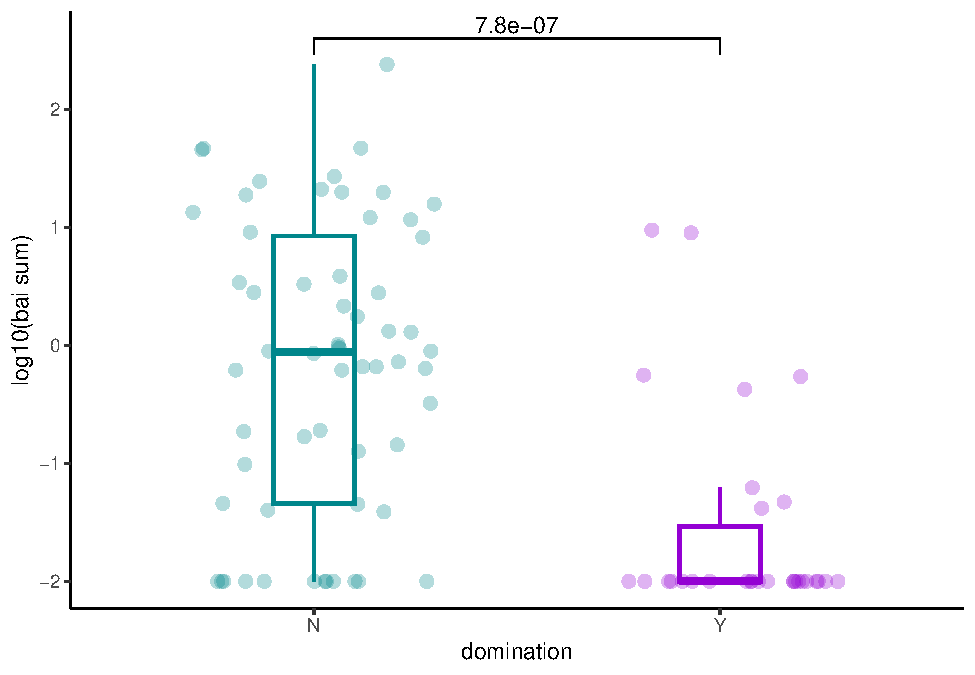
\includegraphics{_main_files/figure-latex/unnamed-chunk-37-1.pdf}

\hypertarget{sbas-and-domination}{%
\section{SBAs and domination}\label{sbas-and-domination}}

\begin{Shaded}
\begin{Highlighting}[]
\NormalTok{pathogens\_pre }\SpecialCharTok{\%\textgreater{}\%} \FunctionTok{inner\_join}\NormalTok{(later\_pools\_final) }\SpecialCharTok{\%\textgreater{}\%} 
  \FunctionTok{ggplot}\NormalTok{(}\FunctionTok{aes}\NormalTok{(}\AttributeTok{x=}\NormalTok{any\_dom, }\AttributeTok{y=}\FunctionTok{log10}\NormalTok{(secondary\_nonUDCA), }\AttributeTok{color=}\NormalTok{any\_dom))}\SpecialCharTok{+}
   \FunctionTok{geom\_boxplot}\NormalTok{(}\AttributeTok{width=}\FloatTok{0.2}\NormalTok{, }\AttributeTok{lwd=}\FloatTok{0.8}\NormalTok{, }\AttributeTok{outlier.shape =} \ConstantTok{NA}\NormalTok{) }\SpecialCharTok{+}
  \FunctionTok{geom\_jitter}\NormalTok{(}\AttributeTok{width=}\FloatTok{0.3}\NormalTok{, }\AttributeTok{alpha=}\FloatTok{0.3}\NormalTok{, }\AttributeTok{size=}\FloatTok{2.5}\NormalTok{)}\SpecialCharTok{+}
  \FunctionTok{ylab}\NormalTok{(}\StringTok{"log10(SBAs*)"}\NormalTok{)}\SpecialCharTok{+}
  \FunctionTok{xlab}\NormalTok{(}\StringTok{"domination"}\NormalTok{)}\SpecialCharTok{+}
  \FunctionTok{theme\_classic}\NormalTok{()}\SpecialCharTok{+}
  \FunctionTok{stat\_compare\_means}\NormalTok{(}\AttributeTok{comparisons=}\FunctionTok{list}\NormalTok{(}\FunctionTok{c}\NormalTok{(}\StringTok{"Y"}\NormalTok{, }\StringTok{"N"}\NormalTok{)),}
                     \AttributeTok{method=}\StringTok{"wilcox.test"}\NormalTok{,}
                     \AttributeTok{correct=}\ConstantTok{FALSE}\NormalTok{)}\SpecialCharTok{+}
  \FunctionTok{scale\_color\_manual}\NormalTok{(}\AttributeTok{values=}\FunctionTok{c}\NormalTok{(}\StringTok{"turquoise4"}\NormalTok{,}\StringTok{"darkviolet"}\NormalTok{))}\SpecialCharTok{+}
  \FunctionTok{theme}\NormalTok{(}\AttributeTok{legend.position=}\StringTok{"none"}\NormalTok{)}
\end{Highlighting}
\end{Shaded}

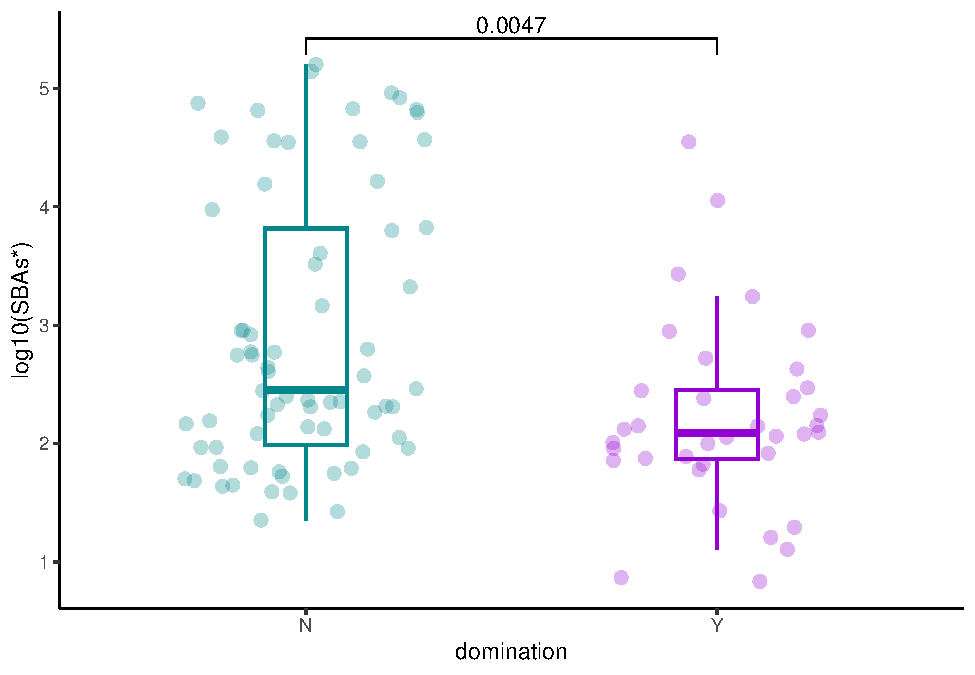
\includegraphics{_main_files/figure-latex/unnamed-chunk-38-1.pdf}

\hypertarget{evaluation-of-udca-exposure-and-clinical-outcomes}{%
\chapter{Evaluation of UDCA exposure and clinical outcomes}\label{evaluation-of-udca-exposure-and-clinical-outcomes}}

\hypertarget{prepare-the-patient-outcome-table}{%
\section{Prepare the patient outcome table}\label{prepare-the-patient-outcome-table}}

\begin{Shaded}
\begin{Highlighting}[]
\FunctionTok{library}\NormalTok{(tidycmprsk)}
\FunctionTok{library}\NormalTok{(ggsurvfit)}
\FunctionTok{library}\NormalTok{(tidycmprsk)}
\FunctionTok{library}\NormalTok{(gtsummary)}

\NormalTok{patients\_urso\_CIF2}\OtherTok{\textless{}{-}}\NormalTok{patients\_urso\_CIF }\SpecialCharTok{\%\textgreater{}\%} 
  \FunctionTok{mutate}\NormalTok{(}\AttributeTok{GRM\_mortality=}\FunctionTok{ifelse}\NormalTok{(death}\SpecialCharTok{==}\NormalTok{F }\SpecialCharTok{\&}\NormalTok{ relapse}\SpecialCharTok{==}\NormalTok{F }\SpecialCharTok{\&}\NormalTok{ pod}\SpecialCharTok{==}\StringTok{"N"}\NormalTok{, }\DecValTok{0}\NormalTok{,}
                              \FunctionTok{ifelse}\NormalTok{(relapse}\SpecialCharTok{==}\NormalTok{T }\SpecialCharTok{|}\NormalTok{ pod }\SpecialCharTok{==}\StringTok{"Y"} \SpecialCharTok{|}\NormalTok{ (cod}\SpecialCharTok{==}\StringTok{"Disease Progression"}\SpecialCharTok{|}\NormalTok{cod}\SpecialCharTok{==}\StringTok{"Recurrence of primary disease"}\SpecialCharTok{|}\NormalTok{cod}\SpecialCharTok{==}\StringTok{"Malignant disease"}\SpecialCharTok{|}\NormalTok{cod}\SpecialCharTok{==}\StringTok{"Relapse"}\NormalTok{),}\DecValTok{2}\NormalTok{,                                  }\FunctionTok{ifelse}\NormalTok{(cod}\SpecialCharTok{==}\StringTok{"GvHD"}\SpecialCharTok{|}\NormalTok{cod}\SpecialCharTok{==}\StringTok{"GvHD/Infection"}\SpecialCharTok{|}\NormalTok{(gvhd}\SpecialCharTok{==}\NormalTok{T }\SpecialCharTok{\&}\NormalTok{ death}\SpecialCharTok{==}\NormalTok{T),}\DecValTok{1}\NormalTok{,}\DecValTok{3}\NormalTok{)))) }\SpecialCharTok{\%\textgreater{}\%} 
  \FunctionTok{mutate}\NormalTok{(}\AttributeTok{GRM\_mortality =} \FunctionTok{ifelse}\NormalTok{(}\FunctionTok{is.na}\NormalTok{(GRM\_mortality),}\DecValTok{3}\NormalTok{,GRM\_mortality)) }\SpecialCharTok{\%\textgreater{}\%} 
  \FunctionTok{mutate}\NormalTok{(}\AttributeTok{GRM\_mortality =} \FunctionTok{factor}\NormalTok{(GRM\_mortality,}\AttributeTok{levels=}\FunctionTok{c}\NormalTok{(}\DecValTok{0}\NormalTok{,}\DecValTok{1}\NormalTok{,}\DecValTok{2}\NormalTok{,}\DecValTok{3}\NormalTok{),}\AttributeTok{labels=}\FunctionTok{c}\NormalTok{(}\StringTok{"Censored"}\NormalTok{, }\StringTok{"GRM"}\NormalTok{, }\StringTok{"Relapse/PoD"}\NormalTok{,}\StringTok{"Other"}\NormalTok{))) }\SpecialCharTok{\%\textgreater{}\%} 
  \FunctionTok{mutate}\NormalTok{(}\AttributeTok{TRM\_mortality=}\FunctionTok{ifelse}\NormalTok{(death}\SpecialCharTok{==}\NormalTok{F }\SpecialCharTok{\&}\NormalTok{ relapse}\SpecialCharTok{==}\NormalTok{F }\SpecialCharTok{\&}\NormalTok{ pod}\SpecialCharTok{==}\StringTok{"N"}\NormalTok{, }\DecValTok{0}\NormalTok{,}
                              \FunctionTok{ifelse}\NormalTok{(relapse}\SpecialCharTok{==}\NormalTok{T }\SpecialCharTok{|}\NormalTok{ pod }\SpecialCharTok{==}\StringTok{"Y"} \SpecialCharTok{|}\NormalTok{ (cod}\SpecialCharTok{==}\StringTok{"Disease Progression"}\SpecialCharTok{|}\NormalTok{cod}\SpecialCharTok{==}\StringTok{"Recurrence of primary disease"}\SpecialCharTok{|}\NormalTok{cod}\SpecialCharTok{==}\StringTok{"Malignant disease"}\SpecialCharTok{|}\NormalTok{cod}\SpecialCharTok{==}\StringTok{"Relapse"}\NormalTok{),}\DecValTok{2}\NormalTok{, }\DecValTok{1}\NormalTok{))) }\SpecialCharTok{\%\textgreater{}\%} 
  \FunctionTok{mutate}\NormalTok{(}\AttributeTok{TRM\_mortality =} \FunctionTok{ifelse}\NormalTok{(}\FunctionTok{is.na}\NormalTok{(TRM\_mortality),}\DecValTok{1}\NormalTok{,TRM\_mortality)) }\SpecialCharTok{\%\textgreater{}\%} 
  \FunctionTok{mutate}\NormalTok{(}\AttributeTok{TRM\_mortality =} \FunctionTok{factor}\NormalTok{(TRM\_mortality,}\AttributeTok{levels=}\FunctionTok{c}\NormalTok{(}\DecValTok{0}\NormalTok{,}\DecValTok{1}\NormalTok{,}\DecValTok{2}\NormalTok{),}\AttributeTok{labels=}\FunctionTok{c}\NormalTok{(}\StringTok{"Censored"}\NormalTok{,}\StringTok{"TRM"}\NormalTok{,}\StringTok{"Relapse/PoD"}\NormalTok{)))}

\FunctionTok{table}\NormalTok{(patients\_urso\_CIF2}\SpecialCharTok{$}\NormalTok{GRM\_mortality)}
\end{Highlighting}
\end{Shaded}

\begin{verbatim}
## 
##    Censored         GRM Relapse/PoD       Other 
##         624         191         386         100
\end{verbatim}

\begin{Shaded}
\begin{Highlighting}[]
\NormalTok{patients\_urso\_CIF2}\SpecialCharTok{$}\NormalTok{GRM\_time }\OtherTok{\textless{}{-}}\NormalTok{ patients\_urso\_CIF2}\SpecialCharTok{$}\NormalTok{OS}
\NormalTok{patients\_urso\_CIF2}\SpecialCharTok{$}\NormalTok{GRM\_time[patients\_urso\_CIF2}\SpecialCharTok{$}\NormalTok{relapse}\SpecialCharTok{==}\NormalTok{T }\SpecialCharTok{\&}\NormalTok{ patients\_urso\_CIF2}\SpecialCharTok{$}\NormalTok{pod}\SpecialCharTok{==}\StringTok{"N"}\NormalTok{] }\OtherTok{=}\NormalTok{ patients\_urso\_CIF2}\SpecialCharTok{$}\NormalTok{relapse\_time[patients\_urso\_CIF2}\SpecialCharTok{$}\NormalTok{relapse}\SpecialCharTok{==}\NormalTok{T }\SpecialCharTok{\&}\NormalTok{ patients\_urso\_CIF2}\SpecialCharTok{$}\NormalTok{pod}\SpecialCharTok{==}\StringTok{"N"}\NormalTok{]}
\NormalTok{patients\_urso\_CIF2}\SpecialCharTok{$}\NormalTok{GRM\_time[patients\_urso\_CIF2}\SpecialCharTok{$}\NormalTok{relapse}\SpecialCharTok{==}\NormalTok{F }\SpecialCharTok{\&}\NormalTok{ patients\_urso\_CIF2}\SpecialCharTok{$}\NormalTok{pod}\SpecialCharTok{==}\StringTok{"Y"}\NormalTok{] }\OtherTok{=}\NormalTok{ patients\_urso\_CIF2}\SpecialCharTok{$}\NormalTok{pod\_time[patients\_urso\_CIF2}\SpecialCharTok{$}\NormalTok{relapse}\SpecialCharTok{==}\NormalTok{F }\SpecialCharTok{\&}\NormalTok{ patients\_urso\_CIF2}\SpecialCharTok{$}\NormalTok{pod}\SpecialCharTok{==}\StringTok{"Y"}\NormalTok{]}
\NormalTok{patients\_urso\_CIF2}\SpecialCharTok{$}\NormalTok{GRM\_time[patients\_urso\_CIF2}\SpecialCharTok{$}\NormalTok{relapse}\SpecialCharTok{==}\NormalTok{T }\SpecialCharTok{\&}\NormalTok{ patients\_urso\_CIF2}\SpecialCharTok{$}\NormalTok{pod}\SpecialCharTok{==}\StringTok{"Y"}\NormalTok{] }\OtherTok{=} \FunctionTok{min}\NormalTok{(patients\_urso\_CIF2}\SpecialCharTok{$}\NormalTok{pod\_time[patients\_urso\_CIF2}\SpecialCharTok{$}\NormalTok{relapse}\SpecialCharTok{==}\NormalTok{T }\SpecialCharTok{\&}\NormalTok{ patients\_urso\_CIF2}\SpecialCharTok{$}\NormalTok{pod}\SpecialCharTok{==}\StringTok{"Y"}\NormalTok{],}
\NormalTok{                                                                                            patients\_urso\_CIF2}\SpecialCharTok{$}\NormalTok{relapse\_time[patients\_urso\_CIF2}\SpecialCharTok{$}\NormalTok{relapse}\SpecialCharTok{==}\NormalTok{T }\SpecialCharTok{\&}\NormalTok{ patients\_urso\_CIF2}\SpecialCharTok{$}\NormalTok{pod}\SpecialCharTok{==}\StringTok{"Y"}\NormalTok{])}

\NormalTok{patients\_urso\_CIF2}\SpecialCharTok{$}\NormalTok{TRM\_time }\OtherTok{\textless{}{-}}\NormalTok{ patients\_urso\_CIF2}\SpecialCharTok{$}\NormalTok{OS}
\NormalTok{patients\_urso\_CIF2}\SpecialCharTok{$}\NormalTok{TRM\_time[patients\_urso\_CIF2}\SpecialCharTok{$}\NormalTok{relapse}\SpecialCharTok{==}\NormalTok{T }\SpecialCharTok{\&}\NormalTok{ patients\_urso\_CIF2}\SpecialCharTok{$}\NormalTok{pod}\SpecialCharTok{==}\StringTok{"N"}\NormalTok{] }\OtherTok{=}\NormalTok{ patients\_urso\_CIF2}\SpecialCharTok{$}\NormalTok{relapse\_time[patients\_urso\_CIF2}\SpecialCharTok{$}\NormalTok{relapse}\SpecialCharTok{==}\NormalTok{T }\SpecialCharTok{\&}\NormalTok{ patients\_urso\_CIF2}\SpecialCharTok{$}\NormalTok{pod}\SpecialCharTok{==}\StringTok{"N"}\NormalTok{]}
\NormalTok{patients\_urso\_CIF2}\SpecialCharTok{$}\NormalTok{TRM\_time[patients\_urso\_CIF2}\SpecialCharTok{$}\NormalTok{relapse}\SpecialCharTok{==}\NormalTok{F }\SpecialCharTok{\&}\NormalTok{ patients\_urso\_CIF2}\SpecialCharTok{$}\NormalTok{pod}\SpecialCharTok{==}\StringTok{"Y"}\NormalTok{] }\OtherTok{=}\NormalTok{ patients\_urso\_CIF2}\SpecialCharTok{$}\NormalTok{pod\_time[patients\_urso\_CIF2}\SpecialCharTok{$}\NormalTok{relapse}\SpecialCharTok{==}\NormalTok{F }\SpecialCharTok{\&}\NormalTok{ patients\_urso\_CIF2}\SpecialCharTok{$}\NormalTok{pod}\SpecialCharTok{==}\StringTok{"Y"}\NormalTok{]}
\NormalTok{patients\_urso\_CIF2}\SpecialCharTok{$}\NormalTok{TRM\_time[patients\_urso\_CIF2}\SpecialCharTok{$}\NormalTok{relapse}\SpecialCharTok{==}\NormalTok{T }\SpecialCharTok{\&}\NormalTok{ patients\_urso\_CIF2}\SpecialCharTok{$}\NormalTok{pod}\SpecialCharTok{==}\StringTok{"Y"}\NormalTok{] }\OtherTok{=} \FunctionTok{min}\NormalTok{(patients\_urso\_CIF2}\SpecialCharTok{$}\NormalTok{pod\_time[patients\_urso\_CIF2}\SpecialCharTok{$}\NormalTok{relapse}\SpecialCharTok{==}\NormalTok{T }\SpecialCharTok{\&}\NormalTok{ patients\_urso\_CIF2}\SpecialCharTok{$}\NormalTok{pod}\SpecialCharTok{==}\StringTok{"Y"}\NormalTok{],}
\NormalTok{                                                                                            patients\_urso\_CIF2}\SpecialCharTok{$}\NormalTok{relapse\_time[patients\_urso\_CIF2}\SpecialCharTok{$}\NormalTok{relapse}\SpecialCharTok{==}\NormalTok{T }\SpecialCharTok{\&}\NormalTok{ patients\_urso\_CIF2}\SpecialCharTok{$}\NormalTok{pod}\SpecialCharTok{==}\StringTok{"Y"}\NormalTok{])}

\NormalTok{patients\_urso\_CIF2 }\OtherTok{\textless{}{-}}\NormalTok{ patients\_urso\_CIF2 }\SpecialCharTok{\%\textgreater{}\%} 
  \FunctionTok{mutate}\NormalTok{(}\AttributeTok{GRM\_mortality\_2yr =} \FunctionTok{ifelse}\NormalTok{(GRM\_time }\SpecialCharTok{\textgreater{}} \DecValTok{24}\NormalTok{,}\DecValTok{1}\NormalTok{,GRM\_mortality), }
         \AttributeTok{GRM\_time\_2yr =} \FunctionTok{ifelse}\NormalTok{(GRM\_time }\SpecialCharTok{\textgreater{}} \DecValTok{24}\NormalTok{,}\DecValTok{24}\NormalTok{,GRM\_time), }
         \AttributeTok{TRM\_mortality\_2yr =} \FunctionTok{ifelse}\NormalTok{(TRM\_time }\SpecialCharTok{\textgreater{}} \DecValTok{24}\NormalTok{,}\DecValTok{1}\NormalTok{,TRM\_mortality), }
         \AttributeTok{TRM\_time\_2yr =} \FunctionTok{ifelse}\NormalTok{(TRM\_time }\SpecialCharTok{\textgreater{}} \DecValTok{24}\NormalTok{,}\DecValTok{24}\NormalTok{,TRM\_time), }
         \AttributeTok{death\_2yr =} \FunctionTok{ifelse}\NormalTok{(OS }\SpecialCharTok{\textgreater{}} \DecValTok{24}\NormalTok{,}\ConstantTok{FALSE}\NormalTok{,death), }
         \AttributeTok{OS\_2yr =} \FunctionTok{ifelse}\NormalTok{(OS }\SpecialCharTok{\textgreater{}} \DecValTok{24}\NormalTok{,}\DecValTok{24}\NormalTok{,OS),}
         \AttributeTok{GRM\_mortality\_2yr =} \FunctionTok{factor}\NormalTok{(GRM\_mortality\_2yr,}\AttributeTok{levels=}\DecValTok{1}\SpecialCharTok{:}\DecValTok{4}\NormalTok{,}\AttributeTok{labels=}\FunctionTok{c}\NormalTok{(}\StringTok{"Censored"}\NormalTok{,}\StringTok{"GRM"}\NormalTok{,}\StringTok{"Relapse/PoD"}\NormalTok{,  }\StringTok{"Other"}\NormalTok{)),  }
         \AttributeTok{TRM\_mortality\_2yr =} \FunctionTok{factor}\NormalTok{(TRM\_mortality\_2yr,}\AttributeTok{levels=}\DecValTok{1}\SpecialCharTok{:}\DecValTok{3}\NormalTok{,}\AttributeTok{labels=}\FunctionTok{c}\NormalTok{(}\StringTok{"Censored"}\NormalTok{,  }\StringTok{"TRM"}\NormalTok{, }\StringTok{"Relapse/PoD"}\NormalTok{)))}

\NormalTok{patients\_urso\_CIF2 }\OtherTok{\textless{}{-}}\NormalTok{ patients\_urso\_CIF2 }\SpecialCharTok{\%\textgreater{}\%} \FunctionTok{mutate}\NormalTok{(}\AttributeTok{donor\_new=}\FunctionTok{ifelse}\NormalTok{(donor\_match}\SpecialCharTok{==}\StringTok{"MMRD"}\NormalTok{, }\StringTok{"haplo"}\NormalTok{, donor\_match))}
\end{Highlighting}
\end{Shaded}

\hypertarget{evaluate-ursodiol-exposure-and-overall-survival}{%
\section{Evaluate ursodiol exposure and overall survival}\label{evaluate-ursodiol-exposure-and-overall-survival}}

\hypertarget{univariable-analysis}{%
\subsection{Univariable analysis}\label{univariable-analysis}}

\begin{Shaded}
\begin{Highlighting}[]
\NormalTok{KM.OS }\OtherTok{\textless{}{-}} \FunctionTok{survfit2}\NormalTok{(}\FunctionTok{Surv}\NormalTok{(OS\_2yr,}\FunctionTok{as.numeric}\NormalTok{(death\_2yr))}\SpecialCharTok{\textasciitilde{}}\NormalTok{ursodiol2,}\AttributeTok{data=}\NormalTok{patients\_urso\_CIF2)}
\NormalTok{KM.OS }\SpecialCharTok{\%\textgreater{}\%} \FunctionTok{ggsurvfit}\NormalTok{() }\SpecialCharTok{+}
  \FunctionTok{add\_censor\_mark}\NormalTok{() }\SpecialCharTok{+}
  \FunctionTok{add\_confidence\_interval}\NormalTok{() }\SpecialCharTok{+}
  \FunctionTok{add\_risktable}\NormalTok{(}\AttributeTok{times=}\FunctionTok{c}\NormalTok{(}\DecValTok{0}\NormalTok{,}\DecValTok{6}\NormalTok{, }\DecValTok{12}\NormalTok{, }\DecValTok{18}\NormalTok{, }\DecValTok{24}\NormalTok{))}
\end{Highlighting}
\end{Shaded}

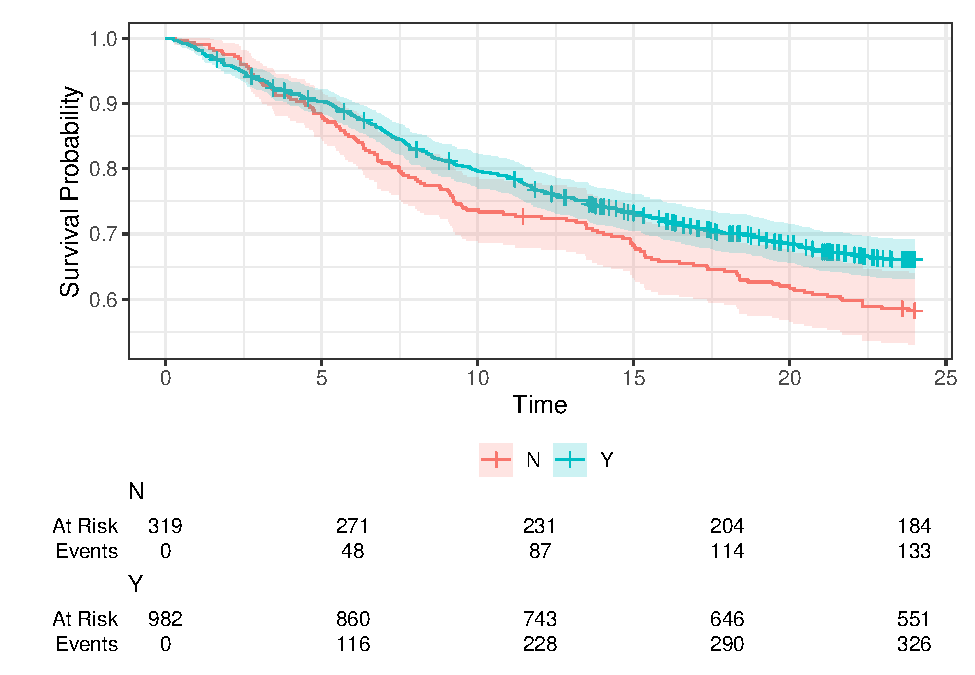
\includegraphics{_main_files/figure-latex/unnamed-chunk-41-1.pdf}

\hypertarget{multivariable-analysis}{%
\subsection{Multivariable analysis}\label{multivariable-analysis}}

\begin{Shaded}
\begin{Highlighting}[]
\NormalTok{coxfit }\OtherTok{\textless{}{-}}\NormalTok{ survival}\SpecialCharTok{::}\FunctionTok{coxph}\NormalTok{(}\FunctionTok{Surv}\NormalTok{(OS\_2yr,}\FunctionTok{as.numeric}\NormalTok{(death\_2yr))}\SpecialCharTok{\textasciitilde{}}\NormalTok{age}\SpecialCharTok{+}\NormalTok{sex}\SpecialCharTok{+}\NormalTok{donor\_match}\SpecialCharTok{+}\NormalTok{graft}\SpecialCharTok{+}\NormalTok{intensity}\SpecialCharTok{+}\NormalTok{ursodiol2,}\AttributeTok{data=}\NormalTok{patients\_urso\_CIF2)}
\NormalTok{coxfit }\SpecialCharTok{\%\textgreater{}\%} \FunctionTok{tbl\_regression}\NormalTok{(}\AttributeTok{exponentiate=}\ConstantTok{TRUE}\NormalTok{) }\SpecialCharTok{\%\textgreater{}\%} \FunctionTok{bold\_p}\NormalTok{()}
\end{Highlighting}
\end{Shaded}

\begin{tabular}{l|c|c|c}
\hline
**Characteristic** & **HR** & **95\% CI** & **p-value**\\
\hline
age & 1.03 & 1.02, 1.04 & \_\_<0.001\_\_\\
\hline
sex &  &  & \\
\hline
F & — & — & \\
\hline
M & 0.95 & 0.79, 1.15 & 0.6\\
\hline
donor\_match &  &  & \\
\hline
haplo & — & — & \\
\hline
haplo/MMUD & 1.20 & 0.57, 2.51 & 0.6\\
\hline
MMRD & 1.23 & 0.16, 9.28 & 0.8\\
\hline
MMUD & 1.23 & 0.73, 2.07 & 0.4\\
\hline
MRD & 0.74 & 0.45, 1.21 & 0.2\\
\hline
MUD & 0.82 & 0.51, 1.32 & 0.4\\
\hline
graft &  &  & \\
\hline
BM & — & — & \\
\hline
CD34 & 0.89 & 0.60, 1.33 & 0.6\\
\hline
PBSC & 1.15 & 0.80, 1.67 & 0.5\\
\hline
UCB & 0.75 & 0.44, 1.28 & 0.3\\
\hline
intensity &  &  & \\
\hline
Ablative & — & — & \\
\hline
Nonablative & 0.49 & 0.33, 0.73 & \_\_<0.001\_\_\\
\hline
Reduced Intensity & 1.00 & 0.74, 1.35 & >0.9\\
\hline
ursodiol2 &  &  & \\
\hline
N & — & — & \\
\hline
Y & 0.69 & 0.55, 0.85 & \_\_<0.001\_\_\\
\hline
\end{tabular}

\hypertarget{evaluation-of-cumulative-incidences}{%
\section{Evaluation of cumulative incidences}\label{evaluation-of-cumulative-incidences}}

\hypertarget{cumulative-incidence-of-gvhd-related-mortality}{%
\subsection{Cumulative incidence of GVHD-related mortality}\label{cumulative-incidence-of-gvhd-related-mortality}}

\begin{Shaded}
\begin{Highlighting}[]
\NormalTok{gray.test.GRM }\OtherTok{\textless{}{-}} \FunctionTok{cuminc}\NormalTok{(}\FunctionTok{Surv}\NormalTok{(GRM\_time\_2yr, GRM\_mortality\_2yr)}\SpecialCharTok{\textasciitilde{}}\NormalTok{ursodiol2, }\AttributeTok{data=}\NormalTok{patients\_urso\_CIF2)}

\NormalTok{gray.test.GRM }\SpecialCharTok{\%\textgreater{}\%} \FunctionTok{tbl\_cuminc}\NormalTok{(}\AttributeTok{times=} \FunctionTok{c}\NormalTok{(}\DecValTok{6}\NormalTok{,}\DecValTok{12}\NormalTok{,}\DecValTok{18}\NormalTok{,}\DecValTok{24}\NormalTok{),}\AttributeTok{outcome=}\StringTok{"GRM"}\NormalTok{) }\SpecialCharTok{\%\textgreater{}\%} 
  \FunctionTok{add\_p}\NormalTok{() }\SpecialCharTok{\%\textgreater{}\%} 
  \FunctionTok{add\_n}\NormalTok{() }\SpecialCharTok{\%\textgreater{}\%} 
  \FunctionTok{modify\_caption}\NormalTok{(}\StringTok{"Outcome: GRM"}\NormalTok{)}
\end{Highlighting}
\end{Shaded}

\begin{table}

\caption{\label{tab:unnamed-chunk-43}Outcome: GRM}
\centering
\begin{tabular}[t]{l|c|c|c|c|c|c}
\hline
**Characteristic** & **N** & **Time 6** & **Time 12** & **Time 18** & **Time 24** & **p-value**\\
\hline
ursodiol2 & 1,301 &  &  &  &  & 0.044\\
\hline
N &  & 7.2\% (4.7\%, 10\%) & 11\% (7.8\%, 15\%) & 14\% (10\%, 18\%) & 16\% (12\%, 20\%) & \\
\hline
Y &  & 3.8\% (2.7\%, 5.1\%) & 8.1\% (6.5\%, 9.9\%) & 10\% (8.2\%, 12\%) & 12\% (9.8\%, 14\%) & \\
\hline
\end{tabular}
\end{table}

\begin{Shaded}
\begin{Highlighting}[]
\NormalTok{gray.test.GRM }\SpecialCharTok{\%\textgreater{}\%} \FunctionTok{ggcuminc}\NormalTok{(}\AttributeTok{outcome=}\StringTok{"GRM"}\NormalTok{) }\SpecialCharTok{+} 
  \FunctionTok{labs}\NormalTok{(}
    \AttributeTok{x =} \StringTok{"Months after HCT"}\NormalTok{,}
    \AttributeTok{y =} \StringTok{"Cumulative Incidence (GRM)"}
\NormalTok{  ) }\SpecialCharTok{+} 
  \FunctionTok{add\_confidence\_interval}\NormalTok{() }\SpecialCharTok{+}
  \FunctionTok{add\_risktable}\NormalTok{(}\AttributeTok{times=}\FunctionTok{c}\NormalTok{(}\DecValTok{0}\NormalTok{,}\DecValTok{6}\NormalTok{,}\DecValTok{12}\NormalTok{,}\DecValTok{18}\NormalTok{,}\DecValTok{24}\NormalTok{))}
\end{Highlighting}
\end{Shaded}

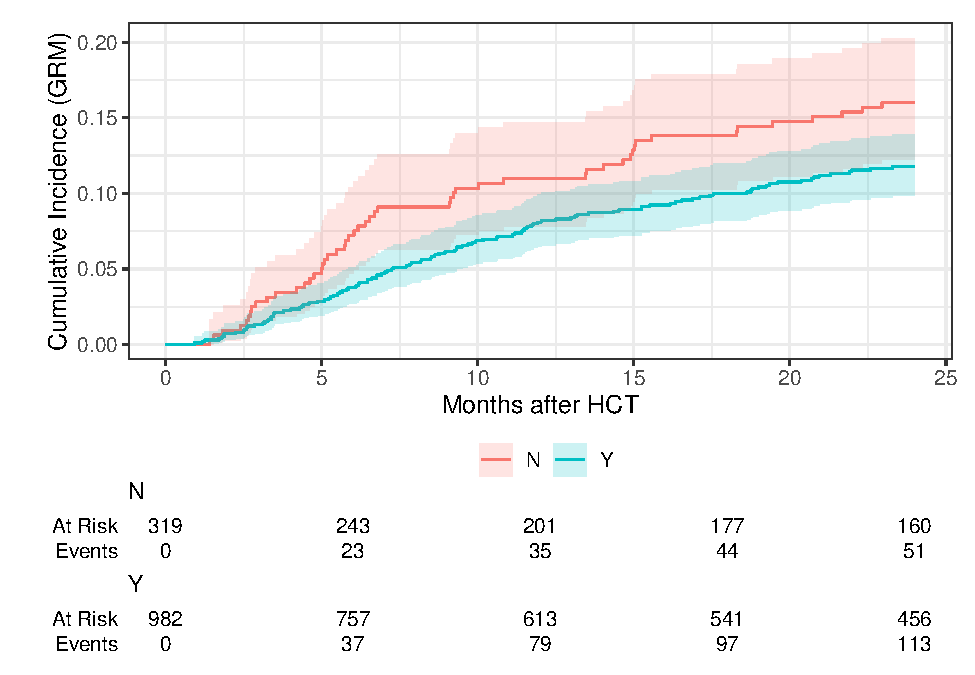
\includegraphics{_main_files/figure-latex/unnamed-chunk-44-1.pdf}

\hypertarget{cumulative-incidence-of-relapseprogression-of-disease}{%
\subsection{Cumulative incidence of Relapse/progression of disease}\label{cumulative-incidence-of-relapseprogression-of-disease}}

\begin{Shaded}
\begin{Highlighting}[]
\NormalTok{gray.test.GRM }\SpecialCharTok{\%\textgreater{}\%} \FunctionTok{tbl\_cuminc}\NormalTok{(}\AttributeTok{times=} \FunctionTok{c}\NormalTok{(}\DecValTok{6}\NormalTok{,}\DecValTok{12}\NormalTok{,}\DecValTok{18}\NormalTok{,}\DecValTok{24}\NormalTok{),}\AttributeTok{outcome=}\StringTok{"Relapse/PoD"}\NormalTok{) }\SpecialCharTok{\%\textgreater{}\%} 
  \FunctionTok{add\_p}\NormalTok{() }\SpecialCharTok{\%\textgreater{}\%} 
  \FunctionTok{add\_n}\NormalTok{() }\SpecialCharTok{\%\textgreater{}\%} 
  \FunctionTok{modify\_caption}\NormalTok{(}\StringTok{"Outcome: Relapse/PoD"}\NormalTok{)}
\end{Highlighting}
\end{Shaded}

\begin{table}

\caption{\label{tab:unnamed-chunk-45}Outcome: Relapse/PoD}
\centering
\begin{tabular}[t]{l|c|c|c|c|c|c}
\hline
**Characteristic** & **N** & **Time 6** & **Time 12** & **Time 18** & **Time 24** & **p-value**\\
\hline
ursodiol2 & 1,301 &  &  &  &  & 0.088\\
\hline
N &  & 12\% (8.9\%, 16\%) & 18\% (14\%, 23\%) & 22\% (17\%, 26\%) & 23\% (18\%, 28\%) & \\
\hline
Y &  & 15\% (13\%, 17\%) & 24\% (21\%, 26\%) & 26\% (24\%, 29\%) & 28\% (25\%, 31\%) & \\
\hline
\end{tabular}
\end{table}

\hypertarget{cumulative-incidence-of-mortality-non-related-to-gvhd-or-relapseprogression-of-disease}{%
\subsection{Cumulative incidence of mortality non-related to GVHD or relapse/progression of disease}\label{cumulative-incidence-of-mortality-non-related-to-gvhd-or-relapseprogression-of-disease}}

\begin{Shaded}
\begin{Highlighting}[]
\NormalTok{gray.test.GRM }\SpecialCharTok{\%\textgreater{}\%} \FunctionTok{tbl\_cuminc}\NormalTok{(}\AttributeTok{times=} \FunctionTok{c}\NormalTok{(}\DecValTok{6}\NormalTok{,}\DecValTok{12}\NormalTok{,}\DecValTok{18}\NormalTok{,}\DecValTok{24}\NormalTok{),}\AttributeTok{outcome=}\StringTok{"Other"}\NormalTok{) }\SpecialCharTok{\%\textgreater{}\%} 
  \FunctionTok{add\_p}\NormalTok{() }\SpecialCharTok{\%\textgreater{}\%} 
  \FunctionTok{add\_n}\NormalTok{() }\SpecialCharTok{\%\textgreater{}\%} 
  \FunctionTok{modify\_caption}\NormalTok{(}\StringTok{"Outcome: Other"}\NormalTok{)}
\end{Highlighting}
\end{Shaded}

\begin{table}

\caption{\label{tab:unnamed-chunk-46}Outcome: Other}
\centering
\begin{tabular}[t]{l|c|c|c|c|c|c}
\hline
**Characteristic** & **N** & **Time 6** & **Time 12** & **Time 18** & **Time 24** & **p-value**\\
\hline
ursodiol2 & 1,301 &  &  &  &  & 0.003\\
\hline
N &  & 4.7\% (2.7\%, 7.4\%) & 7.2\% (4.7\%, 10\%) & 8.8\% (6.0\%, 12\%) & 11\% (7.6\%, 14\%) & \\
\hline
Y &  & 4.1\% (3.0\%, 5.4\%) & 5.0\% (3.8\%, 6.5\%) & 5.4\% (4.1\%, 7.0\%) & 5.6\% (4.3\%, 7.2\%) & \\
\hline
\end{tabular}
\end{table}

\hypertarget{multivariable-analysis-of-gvhd-related-mortality}{%
\subsection{Multivariable analysis of GVHD-related mortality}\label{multivariable-analysis-of-gvhd-related-mortality}}

\begin{Shaded}
\begin{Highlighting}[]
\NormalTok{fgmodel.GRM }\OtherTok{\textless{}{-}} \FunctionTok{crr}\NormalTok{(}\FunctionTok{Surv}\NormalTok{(GRM\_time\_2yr,GRM\_mortality\_2yr)}\SpecialCharTok{\textasciitilde{}}\NormalTok{age}\SpecialCharTok{+}\NormalTok{sex}\SpecialCharTok{+}\NormalTok{donor\_match}\SpecialCharTok{+}\NormalTok{graft}\SpecialCharTok{+}\NormalTok{intensity}\SpecialCharTok{+}\NormalTok{ursodiol2,}\AttributeTok{data=}\NormalTok{patients\_urso\_CIF2)}
\NormalTok{fgmodel.GRM }\SpecialCharTok{\%\textgreater{}\%} \FunctionTok{tbl\_regression}\NormalTok{(}\AttributeTok{exponentiate=}\ConstantTok{TRUE}\NormalTok{) }\SpecialCharTok{\%\textgreater{}\%} \FunctionTok{bold\_p}\NormalTok{()}
\end{Highlighting}
\end{Shaded}

\begin{tabular}{l|c|c|c}
\hline
**Characteristic** & **HR** & **95\% CI** & **p-value**\\
\hline
age & 1.02 & 1.01, 1.04 & \_\_0.002\_\_\\
\hline
sex &  &  & \\
\hline
F & — & — & \\
\hline
M & 0.77 & 0.56, 1.05 & 0.10\\
\hline
donor\_match &  &  & \\
\hline
haplo & — & — & \\
\hline
haplo/MMUD & 1.78 & 0.57, 5.59 & 0.3\\
\hline
MMRD & 0.00 & 0.00, 0.00 & \_\_<0.001\_\_\\
\hline
MMUD & 1.52 & 0.65, 3.58 & 0.3\\
\hline
MRD & 0.58 & 0.26, 1.28 & 0.2\\
\hline
MUD & 0.74 & 0.35, 1.59 & 0.4\\
\hline
graft &  &  & \\
\hline
BM & — & — & \\
\hline
CD34 & 1.28 & 0.59, 2.79 & 0.5\\
\hline
PBSC & 1.64 & 0.85, 3.16 & 0.14\\
\hline
UCB & 0.88 & 0.36, 2.19 & 0.8\\
\hline
intensity &  &  & \\
\hline
Ablative & — & — & \\
\hline
Nonablative & 0.95 & 0.53, 1.71 & 0.9\\
\hline
Reduced Intensity & 1.25 & 0.75, 2.09 & 0.4\\
\hline
ursodiol2 &  &  & \\
\hline
N & — & — & \\
\hline
Y & 0.66 & 0.46, 0.94 & \_\_0.022\_\_\\
\hline
\end{tabular}

  \bibliography{book.bib,packages.bib}

\end{document}
